\documentclass{article}
\usepackage{graphicx} % Required for inserting images
\usepackage{geometry}
\usepackage{amsfonts}
\usepackage{amsmath}
\usepackage{algorithm}
\usepackage{algpseudocode}
\usepackage{algorithmicx}
\usepackage{url}
\usepackage{xspace}
\usepackage{caption}
\usepackage{mathrsfs}
\usepackage{enumerate}
\usepackage{subcaption}
\usepackage{xspace}
\usepackage{hyperref}

\usepackage{easyReview}

\newcommand{\Real}{\mathbb{R}}
\newcommand{\Rd}{\mathbb{R}^d}
\newcommand{\Nat}{\mathbb{N}}
\newcommand{\bx}{\mathbf{x}}
\newcommand{\bv}{\mathbf{v}}
\newcommand{\bX}{\mathbf{X}}
\newcommand{\bQ}{\mathbf{Q}}
\newcommand{\bXpR}{\mathbf{X}'_{\bR}}
\newcommand{\bXpS}{\mathbf{X}'_{\bS}}
\newcommand{\by}{\mathbf{y}}
\newcommand{\br}{\mathbf{r}}
\newcommand{\bs}{\mathbf{s}}
\newcommand{\bR}{\mathbf{R}}
\newcommand{\bS}{\mathbf{S}}
\newcommand{\bP}{\mathbf{P}}
\newcommand{\bxs}{\mathbf{x}^*}
\newcommand{\bq}{\mathbf{q}}
\newcommand{\hR}{h_R}
\newcommand{\hS}{h_S}

\newcommand{\dist}{\mathrm{dist}}
\newcommand{\cosim}{\mathrm{sim}}

\newcommand{\bigO}{\mathcal{O}}
\newcommand{\mH}{\mathcal{H}}
\newcommand{\mN}{\mathcal{N}}
\newcommand{\mB}{\mathcal{B}}
\newcommand{\mBi}{\mathcal{B}_i}
\newcommand{\mC}{\mathcal{C}}
\newcommand{\mT}{\mathcal{T}}
\newcommand{\mF}{\mathcal{F}}
\newcommand{\mS}{\mathcal{S}}
\newcommand{\mSd}{\mathcal{S}^{d-1}}

% \newcommand{\tN}{\widetilde{N}}
\newcommand{\tNq}{\widetilde{N}_\bq}

\newcommand{\ws}{\texttt{WarpSelect}\xspace}

\newcommand{\ip}{iProbes}
\newcommand{\qp}{qProbes}
\newcommand{\pidx}{\mathbf{ProbeIdx}}

\newcommand{\fpp}{Falconn\texttt{++}\xspace}
\newcommand{\lp}{layerProbes\xspace}
\newcommand{\fgpu}{FAISS-GPU\xspace}
\newcommand{\mfpp}{m\fpp}
\newcommand{\glv}{GloVe-100\xspace}
\newcommand{\imgnt}{ImageNet\xspace}
\newcommand{\gist}{GIST\xspace}
\newcommand{\ymlm}{Yahoo-minilm\xspace}

\renewcommand{\Pr}[1]{\textrm{\bf Pr}\left[#1\right]}
\newcommand{\eps}{\varepsilon}
\newcommand{\argmin}{\arg\min}
\newcommand{\argmax}{\arg\max}
\newcommand{\crNN}{$(c, r)$-NN\xspace}
\newcommand{\sgn}{\texttt{sgn}}

\newcommand{\dotqr}{\bq^\top \br}
\newcommand{\dotqx}{\bq^\top \bx}
\newcommand{\dotxr}{\bx^\top \br}
\newcommand{\dotxs}{\bx^\top \bs}
\newcommand{\dotxy}{\bx^\top \by}

\newcommand{\nbx}{\| \bx \|}
\newcommand{\nby}{\| \by \|}

\newcommand{\cf}{CuFalconn\xspace}
% \captionsetup[subfigure]{justification=centering}
\renewcommand{\familydefault}{\sfdefault} % Use Helvetica as the default font

%%%%%%%%%%%%%%%%%%%%%%%%%%%%%%%%
% THEOREMS
%%%%%%%%%%%%%%%%%%%%%%%%%%%%%%%%
% \theoremstyle{plain}
\newtheorem{theorem}{Theorem}[section]
\newtheorem{proposition}[theorem]{Proposition}
\newtheorem{lemma}[theorem]{Lemma}
\newtheorem{corollary}[theorem]{Corollary}
% \theoremstyle{definition}
\newtheorem{definition}[theorem]{Definition}
\newtheorem{assumption}[theorem]{Assumption}
% \theoremstyle{remark}
\newtheorem{remark}[theorem]{Remark}

% \newtheorem{definition}{Definition}

\captionsetup{justification=centering}

\linespread{1.06}

\geometry{
	left=1in,    % Left margin
	right=1in,   % Right margin
	top=1in,     % Top margin
	bottom=1in   % Bottom margin
}

\title{Masters Disseration}
\author{   
    Hugo Phibbs \\
    hphi344@aucklanduni.ac.nz \\
    \small{Repository:} \small\url{https://github.com/HugoPhibbs/CUDA-CEOs}
}
\date{February 2026}

\begin{document}

\maketitle

\begin{abstract}
    
\end{abstract}

\alert{TODO: Write abstract}

\tableofcontents

\alert{Last minute checks: Remove any hand wavy-ness and over-claiming. Make sure themes and notation is coherent.}

\section{Introduction}

Nearest Neighbour Search (NNS) a fundamental problem in computer science. It underpins a wide range of applications including deep learning \cite{dwibedi2021little,chakravarthy2023deep,raj2022estimation,archana2023novel}, data mining \cite{xu2022outlier,sun2022out,dang2021nearest}, recommender systems \cite{sarwar2001item,latifi2022sequential,meng2020pmd,chen2022approximate}, and cyber security \cite{gu2024hierarchical}. Put simply, for a dataset $X$ and a query $\bq$, NNS finds the closest point in $X$ to $\bq$ according to a distance metric $\dist$. A straight-forward solution would be to perform an exhaustive brute force search over all points in $X$ to find the closest to $\bq$. However, for a dataset size $n$ and dimension $d$, this approach has $\bigO(dn)$ complexity. For datasets containing millions of points and large $d$, this complexity is prohibitively slow, even with high performance hardware \cite{weber1998quantitative}. Crucially, in many real world applications, finding the exact nearest neighbours to a query is unnecessary \cite{har2012approximate,halder2024enhancing}. Instead, returning nearest neighbours that are \textit{approximately} close to the query is typically sufficient. Consequently, a large body of research has focused on relaxing exact NNS to \emph{Approximate Nearest Neighbour Search} (ANNS) \cite{indyk1998approximate}, which trades a small loss in accuracy for substantial gains in query speed~\cite{aumuller2023recent}. 

Modern ANNS algorithms are typically divided two separate stages: \emph{indexing} and \emph{querying}. Indexing creates a searchable data structure of $X$ called an index. Querying in turn uses this index to find the closest points in $X$ to $\bq$. Research into ANNS algorithms typically focuses onto creating practical methods that perform well at indexing and querying. Broadly speaking, it's desirable for an index to be both fast to create, and have a minimal memory footprint. Querying in-turn, should be fast, but at the same time, not overly sacrificing accuracy as compared to the ground truth. The efficacy of indexing and querying is interlinked - fast and accurate querying is reliant on the structure and quality of an index.

\paragraph{Introduction to \fpp.} Locality Sensitive Hashing (LSH) is a common approach to the ANNS problem. Essentially, dataset points are indexed into buckets containing other points that are likely to be nearby. When querying, the points in the closest buckets to $\bq$ can be ranked based on their distance to $\bq$ - the closest points being returned as approximate nearest neighbours to $\bq$. A relatively recent extension of LSH is Locality Sensitive Filtering (LSF), whereby points must pass filtering conditions before being added to a bucket. LSF ANNS methods can prove to be more practical by achieving faster querying performance with a smaller index size \cite{christiani2017framework, pham2022falconn++}. An example of this approach is \fpp (2022), introduced by Pham et al. Practically implemented with heuristics inspired from well-grounded theory, \fpp is proven to a more practical ANNS solver - exhibiting accelerated querying speeds for a fixed index size over LSH competitors.

\paragraph{GPU accelerated ANNS.} An emerging trend in ANNS literature is the use of Graphical Processing Units (GPUs) to greatly accelerate both indexing and querying. As compared traditional Central Processing Units (CPUs), GPUs offer an architecture that is well suited to high-throughput, massively parallel computation over large datasets. This essential difference makes is naturally aligned to accelerating ANNS, since they are often reliant on numerically intensive workflows that are easily parallelised. For example, an often decisive factor in determining the speed of an ANNS algorithms are largely independent $d$-dimensional distance computations between data points - a process that a GPU has a clear advantage over CPUs \cite{chang2009compute, chang2008compute, huang2019gpu}. 

\fpp, originally implemented purely on the CPU, is a particularly compelling candidate for GPU acceleration. Much like other ANNS approaches, it built upon processes that are easily parallelised. Additionally, due to it's bucket filtering mechanisms, it has demonstrably superior indexing space complexity than competitors. This is a salient fact, as while GPUs are undoubtedly faster than CPUs for parallel computation, their main memory capacity often comes at a premium to comparable CPU hardware. Consequently, the adaptation of CPU algorithms into GPU equivalents must play close attention to memory usage. 

\paragraph{Contribution.} Motivated by the suitability of \fpp for GPU acceleration, we introduce \textbf{\cf}, a GPU-accelerated $k$ANNS algorithm inspired by \fpp. \cf is designed for a single GPU to compute exact distances to solve ANNS with angular and inner product distance. The indexing stage is a hybrid CPU-GPU approach, while querying is fully resident on the GPU. To our knowledge, \cf represents the first GPU accelerated ANNS method built upon LSF techniques. The method retains the same hashing and filtering mechanisms as \fpp while incorporating several key modifications to better align with GPU architectural constraints, most notably the introduction of a fixed \emph{max} bucket size. Through extensive experimentation on modern large-scale datasets, we demonstrate the robustness and practical applicability of \cf. Furthermore, by benchmarking against established competitor algorithms, we position \cf within the broader landscape of GPU-accelerated ANNS methods.

\alert{I think we need to re-phrase how we use 'inner product distance' in this paper, its MIPS. You're maximising it - not minimising it!}

\paragraph{Paper outline.} This paper first introduces the prerequisite concepts behind \cf. This includes a detailed discussion of the theory of \fpp and how its practically implemented, along with a primer on GPU architecture and programming. Next, we will briefly provide an overview of the surrounding literature of ANNS relevant to \cf. With these foundations established, we then introduce \cf, describing its design motivations and it's practical GPU implementation. Finally, we rigorously evaluate the behaviour of \cf on modern datasets, comparing its performance against the FAISS library \cite{douze2025faiss} and an equivalent CPU implementation.

\section{Preliminaries}

\subsection{Nearest Neighbour Search}
\label{sec:anns}

Consider a dataset $X \subset \Real^d$ containing $n$ points and $d$ dimensions. NNS find the closest point $\bxs \in X$ to a query $\bq$. The point $\bxs$ is thus known as the \emph{nearest neighbour} to $\bq$. The \textit{closeness} of a point and a query is measured by a distance function $\dist : \Real^d \times \Real^d \rightarrow \Real$. The $\dist$ function can take various forms, although commonly it is implemented as angular, inner product or Euclidean (L2) distance. Eq.~\ref{eq:nns_def} formalises the idea of a nearest neighbour. The closely related $k$NNS problem finds the set of the closest $k$ nearest neighbours to a query $\bq$. A graphical explanation of NNS and $k$NNS is given in Fig.~\ref{fig:nns-example}.

\begin{equation}
\bxs = \arg\min_{\bx \in X} \dist(\bx, \bq)
\label{eq:nns_def}
\end{equation}

\begin{figure}
    \centering
    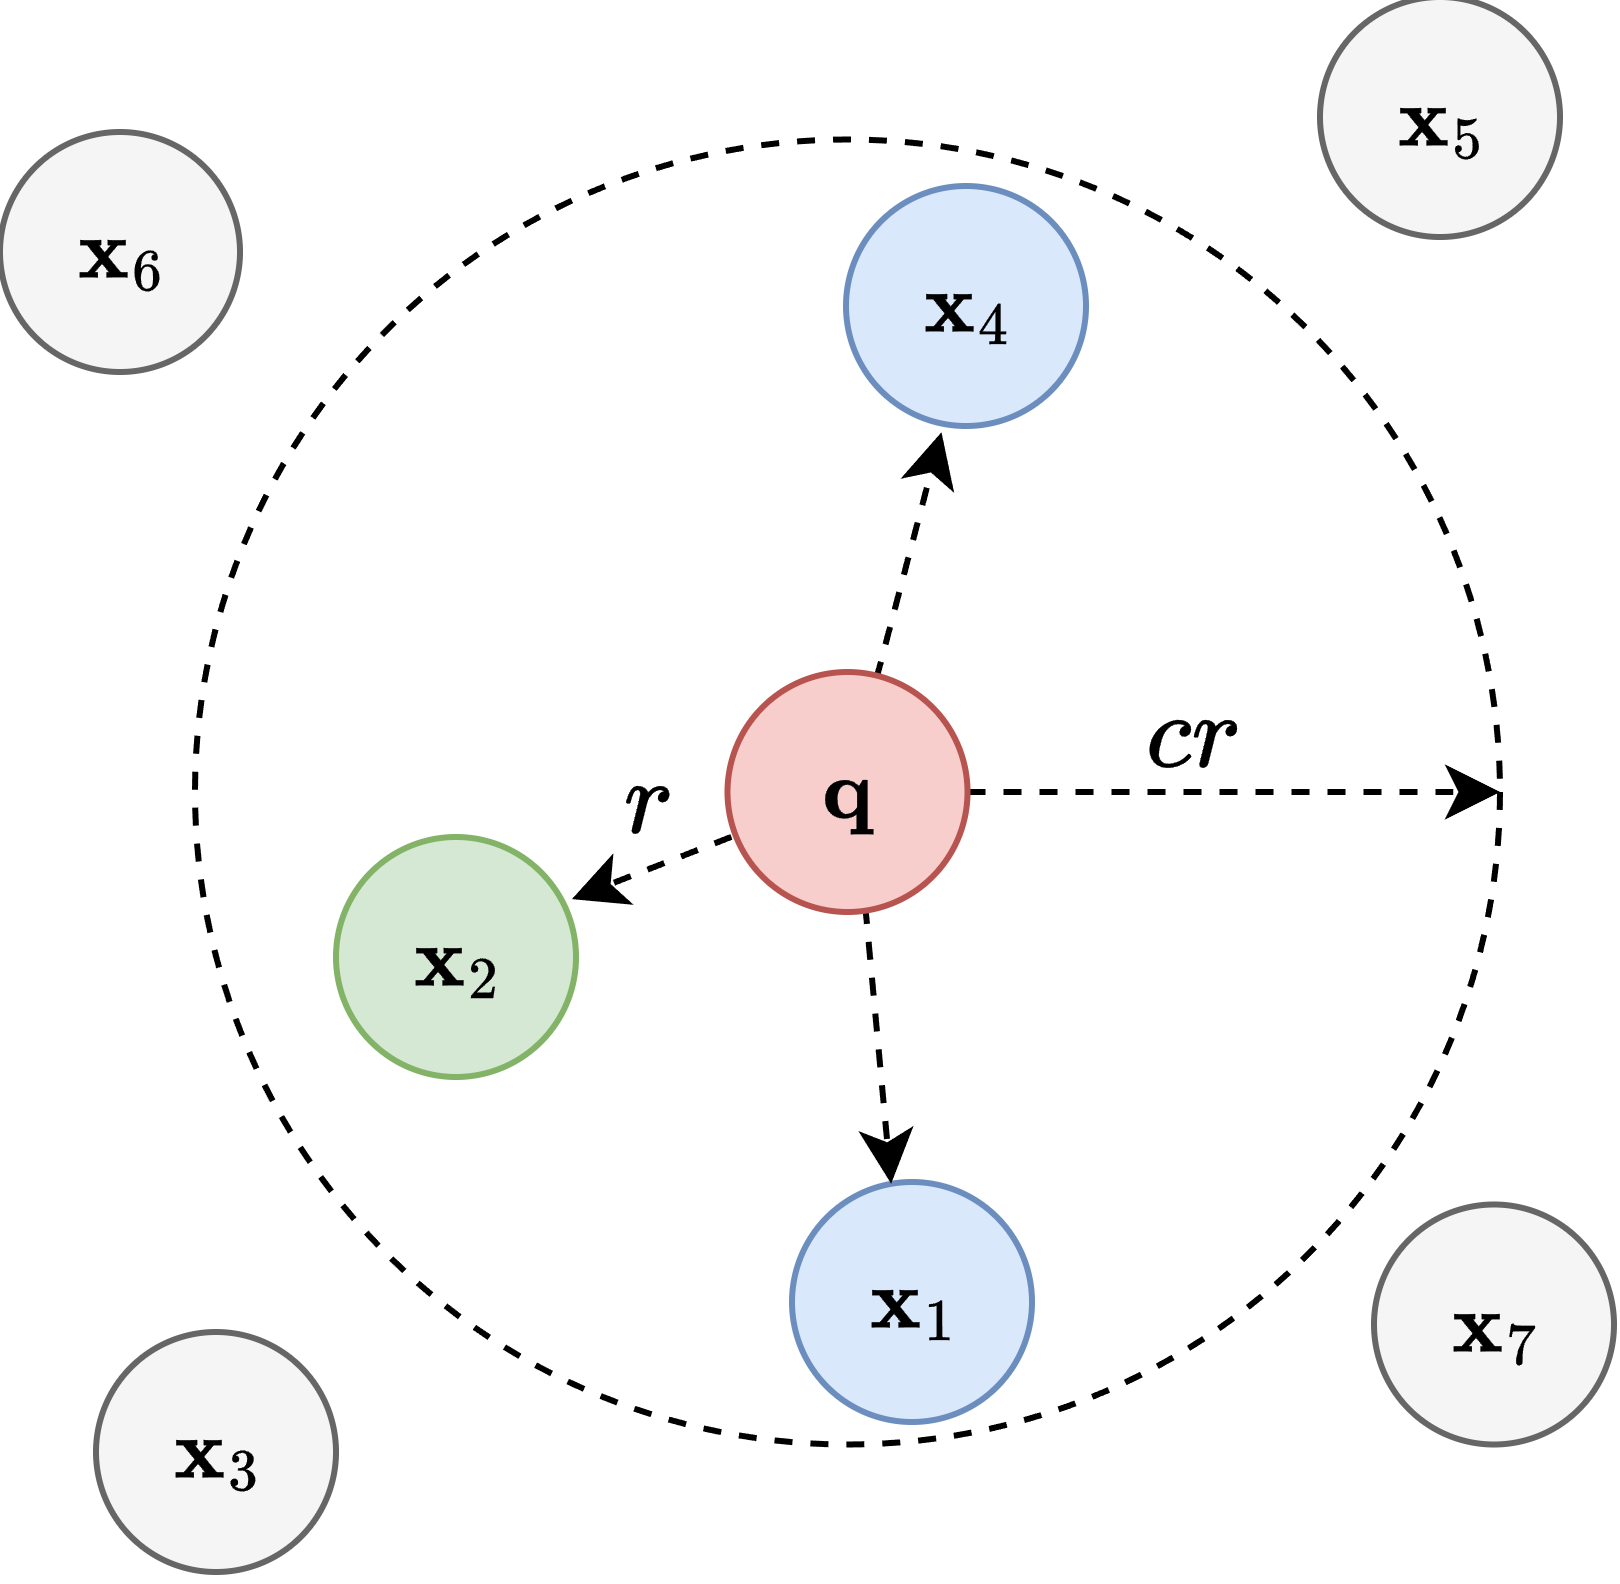
\includegraphics[width=0.5\linewidth]{figs/diags/nns.png}
    \caption{Illustration of the NNS and $k$NNS problem using L2 distance. \\ Here $\bx_{2}$ is the nearest neighbour to $\bq$ and $\{ \bx_{1}, \bx_{2}, \bx_{4}, \bx_{7} \}$ are the $k=4$ nearest neighbours to $\bq$.}
    \label{fig:nns-example}
\end{figure}

As discussed, ANNS is often prefered to an \textit{approximate} NNS for modern practical applications. To define ANNS, given an approximation factor $c > 1 \in \Real$, ANNS returns a point $\bx' \in X$ whose distance to the query is at most a factor $c$ larger than that of the true nearest neighbour, as defined in Eq.~\ref{eq:anns_def}. This notion extends directly to the $k$-nearest neighbour case: $k$ANNS returns $k$ points whose distances to the query $\bq$ are within the same approximation bound. A graphical explanation of this ANNS using Euclidean distance is shown in Fig.~\ref{fig:nns-example}. For a query $\bq$, distance to it's true nearest neighbour $\bx_3$ equal to $r$, and $c > 1$. The set $\tNq =  \{\bx_1, \bx_2, \bx_4\}$ contains all points within $cr$ distance of $\bq$, thus are \emph{approximate} nearest neighbours to $\bq$. Any two points from $\tNq$ would solve the $k$ANNS problem for $\bq$ given $k=2$. 

\begin{equation}
\dist(\bx', \bq) \leq c \cdot \dist(\bxs, \bq)
\label{eq:anns_def}
\end{equation}

The \emph{accuracy} of a $k$ANNS method is typically measured using \emph{recall}. For a given $k$ and query $\bq$, the recall $R_\bq@k$ measures the proportion of the points returned by ANNS that are the true nearest neighbours to $\bq$. Formally, if $\tNq$ and $N_\bq$ containing the approximate and exact $k$ nearest neighbours to $\bq$ then $R@k$ can be defined using Eq.~\ref{eq:recall}. In practical settings, queries are often executed in batches of size $n_q$, and recall is therefore reported as the average $R@k$ across all queries. For a given dataset, an often shared goal of ANNS algorithms is to reduce query time over a range of fixed recall values.

\begin{equation}
    \label{eq:recall}
    \begin{aligned}
    R_\bq@k = \frac{1}{k}\left|\tNq \cap N_\bq \right| \; , \; R@k = \frac{1}{n_q}\sum_{\bq} R_\bq@k
    \end{aligned}
\end{equation}


\subsection{Locality Sensitive Hashing}
\label{sec:lsh}

Locality Sensitive Hashing (LSH) \cite{jafari2021survey} is a widely used approach for ANNS. It delivers guaranteed \emph{sub-linear} query time for the the $(c,r)$-approximate near neighbour problem (\crNN). For a radius $r$ and an approximation factor $c$, the \crNN problem asks to return any point $\bx$ within distance $cr$ to $\bq$ \emph{if} there exists a point $\bxs$ within distance $r$ to $\bq$ \cite{pham2022falconn++}, otherwise return nothing. Although \crNN isn't strictly the same problem as ANNS, it's often the case in literature to solve \crNN as a proxy for ANN, particularly when using LSH \cite{jafari2021survey,huang2015query}. Figure \ref{fig:lsh} shows how LSH could be used for $k$ANNS. With this being said, we can formally define LSH using Def.~\ref{def:LSH}.

\begin{definition}[LSH]
    \label{def:LSH}
	For a distance function $\dist$, positive reals $r$, $c$, $p_1$, $p_2$, and $0 < p_2 < p_1 \leq 1$, $c > 1$, a family of hash functions $\mH$ is \emph{$(r,cr,p_1,p_2)$-sensitive} if for uniformly chosen $h \in \mH$ and all $\bx, \by, \bq \in \Rd$:
	\begin{itemize}%[leftmargin=4ex]
		\item If $\dist(\bx, \bq) \leq r$, then  $\Pr{h(\bx)=h(\bq)} \geq p_1$ ;
		%		\vspace{-0.5mm}
		\item If $\dist(\by, \bq) \geq cr$, then  $\Pr{h(\by)=h(\bq)} \leq p_2$ .
	\end{itemize}
\end{definition}

% \paragraph{Concanation}    

% We need $k$ concanating hash functions to form a new LSH families, then we have $p_1^k$ for close points, and $p_2^k$ for far away points.
% How to set the value for $k$?

% We set $p_2^k = 1/n$ so that we expect in the worst case $n * p_2^k = O(1)$ far away point colliding with $q$
% Then $k = log(n) / log(1/p_2)$

% Then we have $p_1^k = n^{-log{(1/p1)} / log(1/p2)}$, there fore we need to repeat $L = 1/p_1^k = n^{log{(1/p1)} / log{(1/p2))}}$ tables to ensure the collision of close point in at least one table.

% If using Simhash, $L = n^{1/c}$
% If using Falconn, $L = n^{1/c^2}$

\paragraph{Hashing mechanism.}
For a given hash function $h$ and point $\bx$, $h(\bx)$ is called the \emph{hash value} of $\bx$ under $h$. A hash \emph{collision} between two points occurs when they share the same hash value. Given a query point $\bq$, a collision with a point $\bx$ is called a \emph{true collision} if $\dist(\bx,\bq) \le r$, and a \emph{false collision} if $\dist(\bx,\bq) \ge cr$. Given this 

The central driving property of a locality-sensitive hash (LSH) function is that true collisions occur with higher probability than false collisions. This property motivates the use of LSH to construct searchable indices for ANNS.

To this end, consider an LSH function $h$ with $D$ distinct outputs. These outputs can thus be assigned unique labels in $[D]$, i.e.\ $h : \Rd \rightarrow [D]$. Applying $h$ to each point $\bx \in X$ assigns it a label $i = h(\bx)$. Points with the same label are grouped into sets called \emph{hash buckets}. We say that a point $\bx$ is \emph{hashed} to bucket labelled $\mB_i$ if $h(\bx) = i$. The collection of the $D$ buckets induced by $h$ is collectively called a \emph{hash table} $\mT$ (see Eq.~\ref{eq:lsh_tab}). By the definition of LSH, these buckets are more likely to contain pairs of close points than far points, and the hash table may therefore be interpreted as a coarse partitioning of $X$ based on proximity measured by $\dist$.

\begin{equation}
\label{eq:lsh_tab}
\begin{aligned}
\mT &= \{ \mB_1, \mB_2, \dots, \mB_D \}, \quad
\text{where}\quad \mB_i &= \{ \bx \in X \mid h(\bx) = i \}.
\end{aligned}
\end{equation}

\paragraph{A practical LSH approach:} A naive approach to use an LSH based ANNS method would be to construct a just one hash table using one hash function. This however, has several drawbacks. Firstly, there is a non-trivial bounding probability $p_2$ that the hash function creates false collisions. To mitigate this issue, a typical approach is to \emph{concatenate} $l$ independent LSH hash functions together into a combined hash function $g$, where:

\begin{equation}
    \label{eq:lsh-concat}
    \begin{aligned}
    g(\bx) = (h_1(\bx), h_2(\bx), \dots, h_l(\bx))
    \end{aligned}
\end{equation}

Two points $\bx$ and $\bq$ only collide when they have identical hashes across $h_1, h_2, \dots, h_l$. Since there are $D$ unique outputs for a given $h_i$, $g(\bx)$ effectively creates a choice of $D^l$ buckets that a point can be assigned to. This then bounds the chance of a false collisions by $p^l_2$. However, concatenating hash functions also \emph{decreases} the chance of a true collision to $p^l_1$. To address this issue, combine $L$ hash tables, each with a concatenated hash function $g_i$, for $i \in [L]$. For two points to collide, they have to have the same hash value on just one hash table. 

Using $L$ tables decreases the probability of missing a true collision from $1-p^l_1$ to $(1-p^l_1)^L$. Thus the probability of a true hash collision across $L$ tables \emph{increases} to $1-(1-p^l_1)^L \approx 1 - e^{- L \cdot p^l_1} $.

% Assume $p_2$ and $l$ are chosen such that there is a negligible chance of a false hash collision per table.

% To ensure a constant probability of a false collision, set $p^l_2 = 1/n$.

\paragraph{LSH parameter setting.}
With these choices in mind, to obtain a practical \crNN solver, we first select $p_2$ and $l$ such that the probability of a false hash collision per table is negligible. Concretely, we set $p_2^l = 1/n$, which yields $l = \ln n / \ln(1/p_2)$. Since $l$ grows logarithmically with $n$, the single-table true collision probability, $p_1^l$, decreases as $n$ increases. To account for this effect, set $L = O(1/p_1^l)$. The probability of a true hash collision is then:

\[
1-(1-p^l_1)^L \approx 1 - e^{- L \cdot p^l_1} = 1 - e^{-1}
\]

This ensures a constant, non-vanishing probability of a true hash collision across $L$ tables for any $n$. Introducing the exponent $\rho = \ln(p_1)/\ln(p_2)$, this yields an LSH index with $L = \bigO(n^\rho)$ tables. To find a close point with constant probability thus requires sub-linear $\bigO(n^\rho)$ distance computations. 

Minimising the factor $\rho$ is a deciding factor on the practicality of an LSH \crNN method - it dictates the complexity of the indexing space and the necessary number of distance computations (often a dominating factor in the speed of query processing). The LSH family used by a particular family naturally have different collision probabilities $(p_1,p_2)$ for given $(c,r)$, and therefore lead to different values of $\rho$. Accordingly, different \crNN methods have varying indexing and querying complexities, which impact their practical applicability.

\begin{figure}
    \centering
    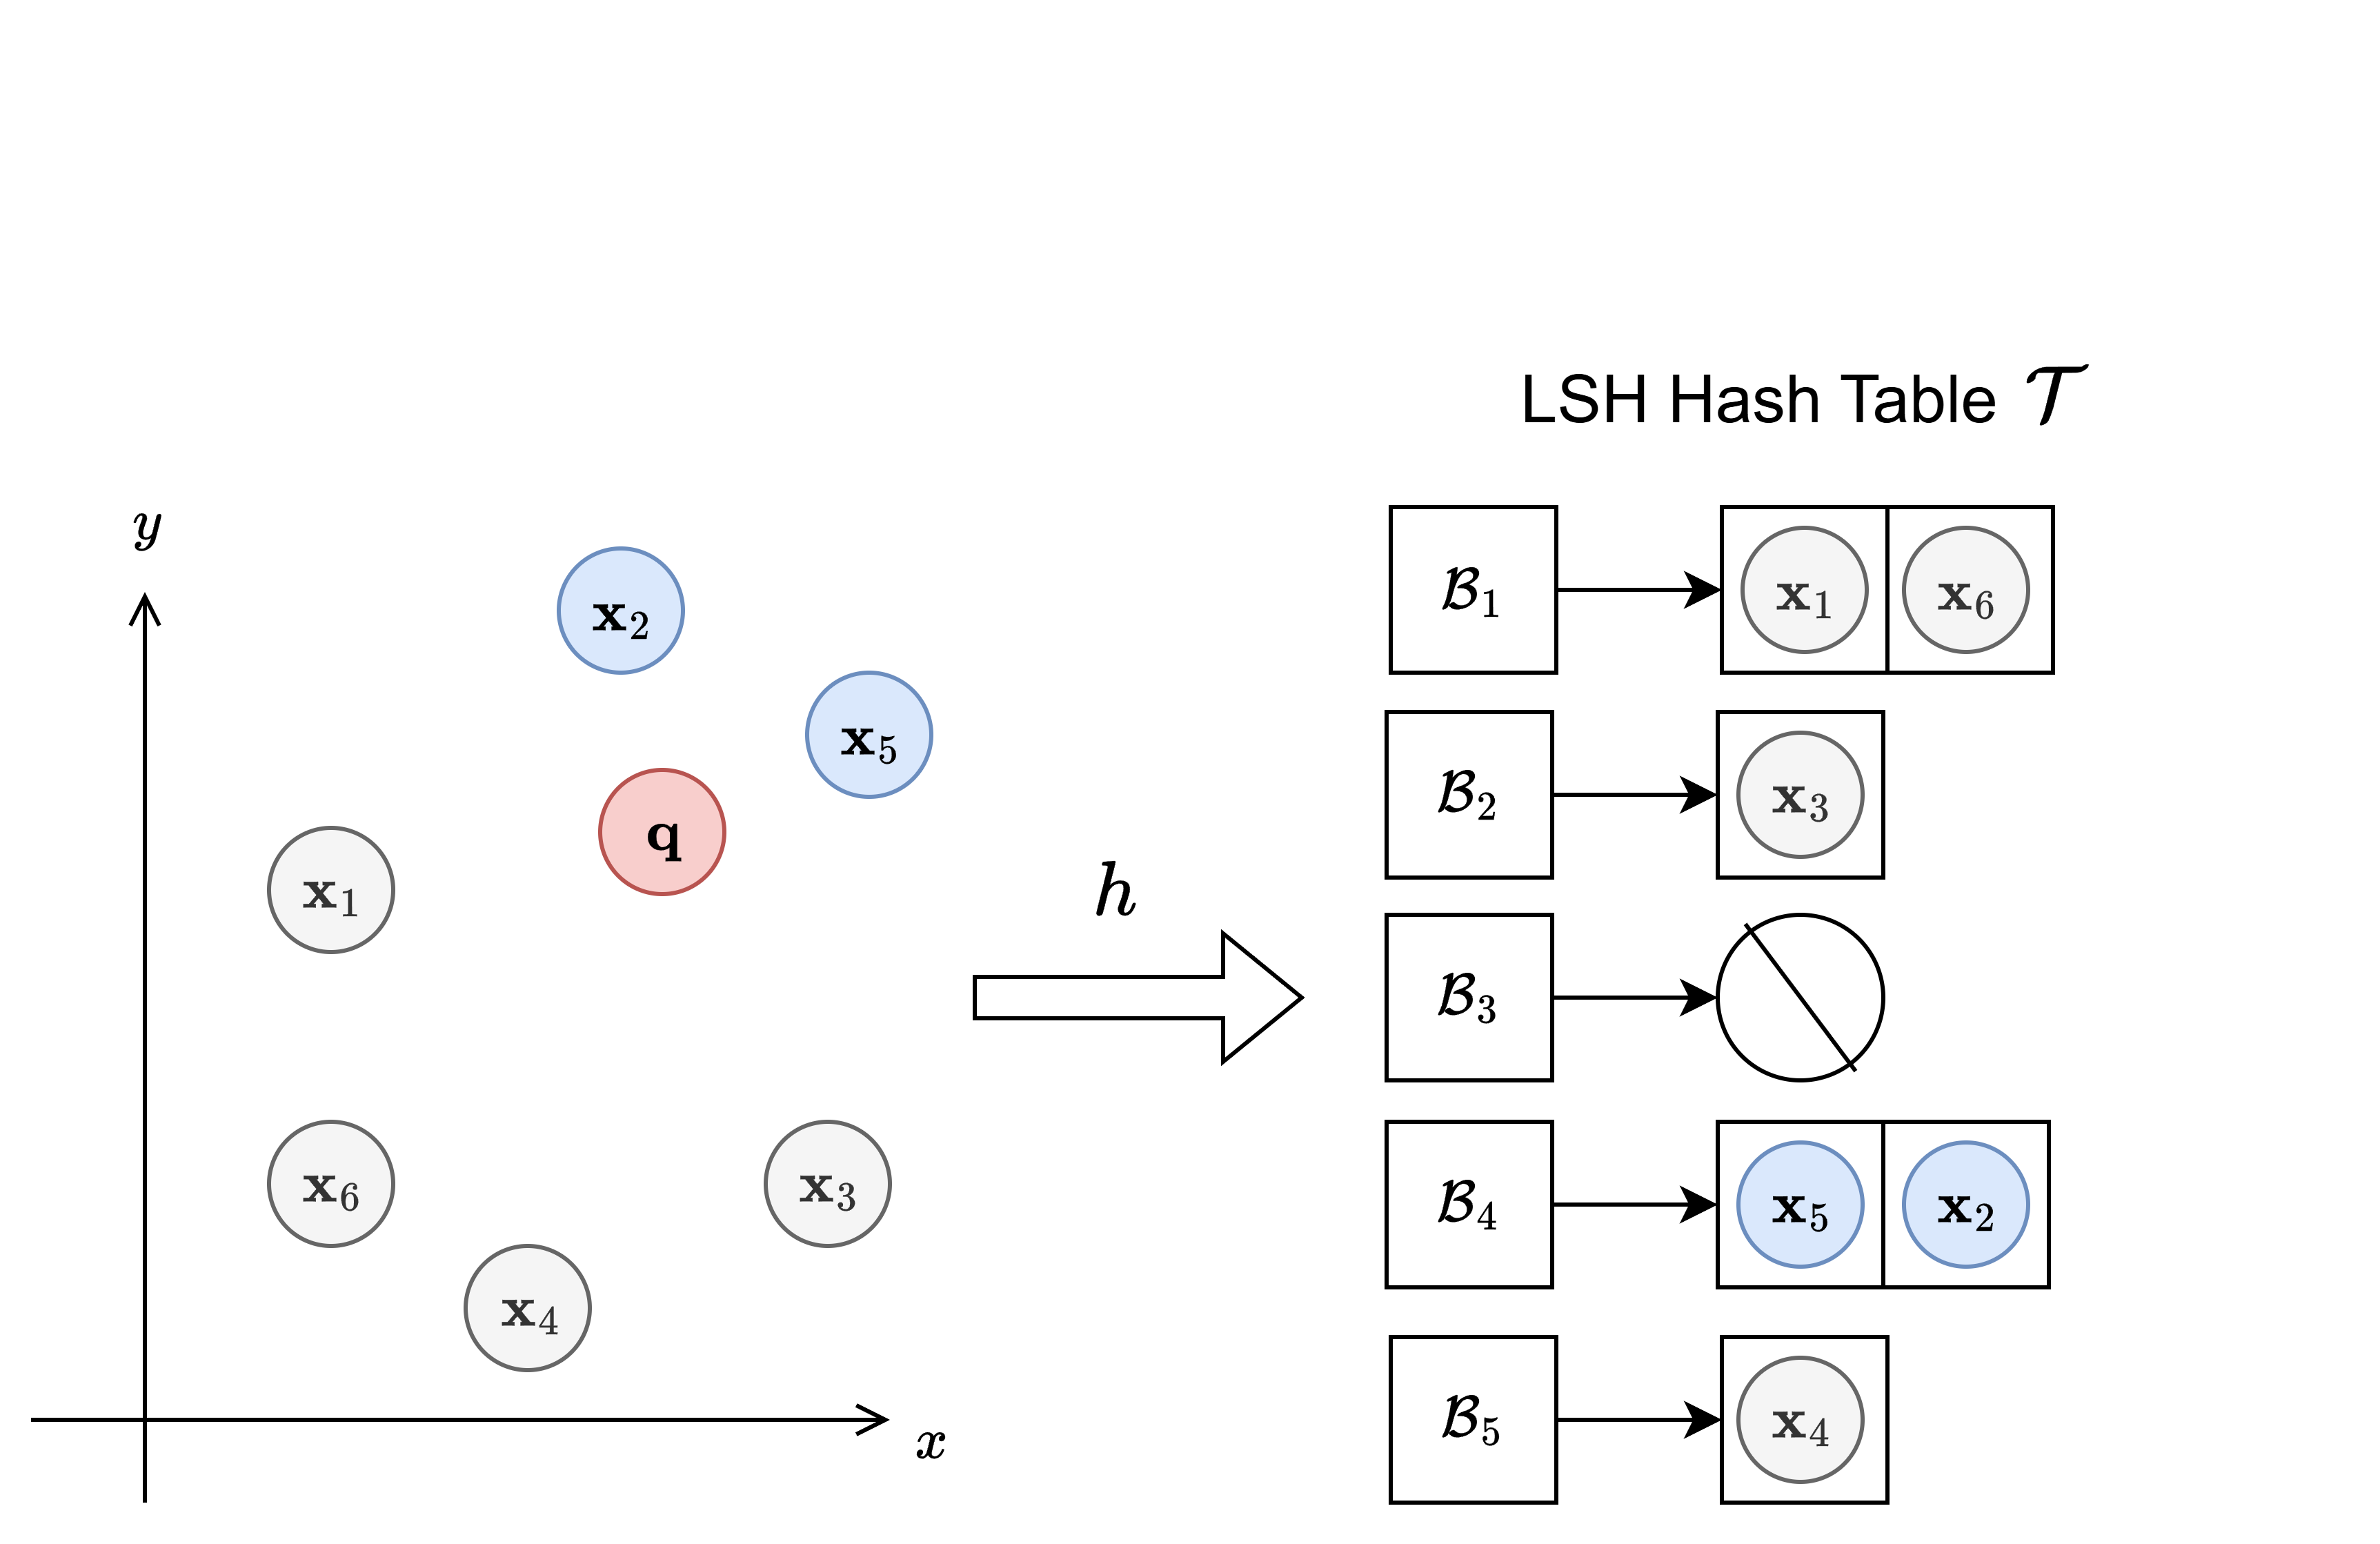
\includegraphics[width=0.8\linewidth]{figs/diags/lsh.png}
    \caption{A simplified example of an LSH hash table for $kANNS$. This uses one hash function creating $D=5$ buckets. If the query $\bq$ hashes to the bucket $\mB_{4}$, then its true $k=2$ nearest neighbours shaded in blue will be found.}
    \label{fig:lsh}
\end{figure}

\subsection{LSH families for angular distance}

This section studies the values of $\rho$ of common LSH families for angular distance for the \crNN problem, including SimHash~\cite{charikar2002similarity} and Falconn~\cite{andoni2015practicaloptimallshangular}. Before we introduce SimHash and Falconn formally, we will give an introduction to angular distance and an embedding trick to simplify the study of $\rho$. The angular distance $\theta_{\bx \by} \in [0, \pi]$ between two vectors $\bx$ and $\by$ is given as:

\begin{equation}
    \theta_{\bx \by} = \arccos\!\left(\frac{\bx^\top \by}{\nbx \nby}\right)
\end{equation}

We can then define the cosine similarity between $\bx$ and $\by$ as:

\begin{equation}
    \cosim(\bx, \by) = \cos(\theta_{\bx \by}) = \frac{\bx^\top \by}{\nbx \nby}
\end{equation}

Maximising cosine similarity is equivalent to minimising angular distance. For ease of notation when deriving different $\rho$, we can embed Euclidean distance on the unit sphere into cosine similarity. Thus minimising Euclidean distance on the unit-sphere is shown to be equivalent to minimising angular distance. To illustrate, take $\bx, \by \in \Rd$, with $\|\bx\|=\|\by\|=1$. Using the inner product expansion of Euclidean distance we can write:

\begin{equation}
    \|\bx-\by\|^2 = \|\bx\|^2 + \|\by\|^2 - 2 \dotxy = 2 - 2\dotxy
\end{equation}

Then:

\begin{equation}
    \bx^\top \by = 1 - \frac{ \|\bx-\by\|^2}{2}
\end{equation}

In the same vein, since $\bx$ and $\by$ are unit vectors, we can write their cosine similarity as:

\begin{equation}
    \cosim(\bx, \by) = \dotxy
\end{equation}

Hence we can embed the Euclidean distance between $\bx$ and $\by$ using: 

\begin{equation}
    \cosim(\bx, \by) = 1 - \frac{\|\bx-\by\|^2}{2}.
\end{equation}

Consequently, minimising Euclidean distance on the unit-sphere is equivalent to maximising cosine similarity. Thus, the study of $\rho$ is equivalent in both regimes. For the \crNN problem, we can then derive the following expressions of equivalence between Euclidean distance and cosine similarity for close and far vectors. 

\begin{equation}
    \label{eq:lsh-t1}
    \bx, \by \quad \text{close: } \|\bx-\by\| \le r
    \quad\Rightarrow\quad \cosim(\bx, \by) \ge t_1 = 1 - \frac{r^2}{2} 
\end{equation}

\begin{equation}
    \label{eq:lsh-t2}
    \bx, \by \quad \text{far: } \|\bx-\by\| \le cr
    \quad\Rightarrow\quad \cosim(\bx, \by) \geq t_2 = 1 - \frac{ c^2r^2}{2}
\end{equation}

\subsubsection{SimHash}
\label{sec:simhash}

We will briefly introduce SimHash's hashing mechanism, the collision probability, and hence derive an exponent $\rho_{SH}$. 

\paragraph{Hashing.} Draw a random vector $\br_a \cosim \mN(0,I_d)$. For a unit vector $\bx \in \mSd$, the hash value $h_a(\bx)$ is given as:

\[
h_a(x) = \operatorname{sign}( \bx^\top \br_a).
\]

\paragraph{Collision Probability.} Two points $\bx$ and $\by$ collide \emph{iff} they lie on the same hyperplane through the origin defined by $\br_a$. Using this definition of $h_a$, the hash collision probability can be derived. For $\bx, \by \in \mSd$, we can denote their angular distance as $\theta_{\bx \by}$. The collision probability between $\bx$ and $\by$ depends only on $\theta_{\bx \by}$. Consequently, we can re-express this using cosine similarity.

\[
\Pr{h_a(x)=h_a(y)}
=
1 - \frac{\theta_{\bx \by}}{\pi}
=
1 - \frac{\arccos(\cosim(\bx, \by))}{\pi}.
\]

Using the cosine similarity thresholds $t_1$ and $t_2$ in Eqs.~\ref{eq:lsh-t1} and \ref{eq:lsh-t2}. We can then derive the close and far collision probabilities based on Euclidean distance:

\[
p_1 = 1 - \frac{\arccos\!\left(1-\frac{r^2}{2}\right)}{\pi},
\qquad
p_2 = 1 - \frac{\arccos\!\left(1-\frac{c^2 r^2}{2}\right)}{\pi}.
\]

\paragraph{Small distance regime ($r \to 0$).} Use a Maclaurin expansion of $cos(\theta)$, for $\theta = \arccos(1 - r^2/2)$. We can then derive approximate forms of $p_1$ and $p_2$, hence derive $\rho_{SH}$: 

\alert{double check this maclaurin, why do we bother with $cos(\theta)$ when we take $\theta$ as an arccos anyways?}

% \[
% \arccos(1-\varepsilon)
% =
% \sqrt{2\varepsilon}
% + O(\varepsilon^{3/2}).
% \]

% With $\varepsilon=r^2/2$ we obtain

% \[
% \arccos\!\left(1-\frac{r^2}{2}\right)
% =
% r + O(r^3),
% \]

% \[
% \arccos\!\left(1-\frac{c^2 r^2}{2}\right)
% =
% cr + O(r^3).
% \]

\[
p_1 = 1 - \frac{r}{\pi} + \bigO(r^3),
\qquad
p_2 = 1 - \frac{cr}{\pi} + \bigO(r^3).
\]

% Using

% \[
% \log\!\left(\frac{1}{1-x}\right)=x+O(x^2),
% \]

% we get

Therefore:

\[
\rho_{SH}
=
\frac{\log(1/p_1)}{\log(1/p_2)}
=
\frac{r/\pi + \bigO(r^2)}{cr/\pi + \bigO(r^2)}
=
\frac{1}{c} + \bigO(r).
\]

\medskip

Given this derivation of $\rho_{SH}$, we can present the following thereom:

\begin{theorem}[LSH exponent of SimHash]
    For Euclidean \crNN on the unit sphere and equivalently for angular distance, SimHash has an exponent $\rho_{SH}$ satisfying:

    \[
    \rho_{SH} \approx \frac{1}{c}
    \quad \text{as } r \to 0.
    \]
\end{theorem}

\subsubsection{Falconn}

Falconn is similar in spirit to SimHash - it relies on projections onto Gaussian random vectors; however, its hashing construction differs fundamentally, leading to distinct theoretical guarantees. As with the preceding discussion of SimHash, we first outline the hashing mechanism, then examine the associated collision probabilities, and finally derive the exponent $\rho$.

\paragraph{Hash function.}
Let $\bx \in \mSd$. Take a set of $D$ random vectors $R \subset \Rd$ with entries sampled from $\mN(0, 1)$. For a point $\bx$, the \emph{score} with respect to a direction $\br \in \widehat{R} = R \cup -R$ \footnote{Where $-R = \{ -\br \mid \br \in R \}$} is defined as the absolute value of the projection $|\bx^\top \br|$. The bucket to which $\bx$ is assigned is determined by the direction $\br_a, a \in [2D]$ achieving the maximum score. Given this, the hash value of $\bx$ and hence the hash function $h$ can be defined using Eq.~\ref{eq:falconnhash}. Consequently, $h$ can take one one of $[2D]$ different values. An illustration of Falconn hashing is shown in Fig.~\ref{fig:falconnhash}. 

\begin{equation}
    \label{eq:falconnhash}
    h(\bx) = \begin{cases}
    a\, \text{if } \sgn(\dotxr_a) \geq 0 \, ,\\
    D + a \, \text{otherwise} \, .
    \end{cases}
\end{equation}

\paragraph{Collision Probability.} The collision probability depends on the angle $\theta_{\bx \by}$ between $\bx$ and $\by$. Following derivation steps, we can yield this in-terms of a cosine similarity value $t$:

\[
\Pr{h(\bx)=h(\by)}
=
D^{-(1-t)/(1+t)}
\quad \text{as } D \to \infty.
\]

Using the thresholds $t_1$ and $t_2$ for close and far points in Eqs.\ref{eq:lsh-t1} and \ref{eq:lsh-t2}, we can derive $p_1$ and $p_2$ as in-terms of Euclidean distance:

\[
p_1 = D^{-r^2/(4-r^2)},
\qquad
p_2 = D^{-c^2 r^2/(4-c^2 r^2)}.
\]

\paragraph{Small distance regime ($r\to0$).} Using a Maclaurin expansion of $x$ where $x = r^2/4$. As $r$ vanishes, we can derive an exponent $\rho$: 

% \[
% \frac{r^2}{4-r^2}
% =
% \frac{r^2}{4}+O(r^4),
% \qquad
% \frac{c^2 r^2}{4-c^2 r^2}
% =
% \frac{c^2 r^2}{4}+O(r^4).
% \]

% Therefore:

\[
\rho
=
\frac{\log(1/p_1)}{\log(1/p_2)} = 
\frac{r^2/4 + O(r^4)}{c^2 r^2/4 + O(r^4)}
=
\frac{1}{c^2}+O(r^2).
\]

\medskip

Given this derivation of $\rho$, we can present the following thereom:

\begin{theorem}[LSH Exponent of Falconn]
For Euclidean \crNN on the unit sphere and equivalently for angular distance, Falconn has a exponent $\rho$ satisfying:

\[
\rho \approx \frac{1}{c^2} \quad\text{as } r\to0.
\]

\end{theorem}

\begin{figure}
    \centering
    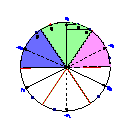
\includegraphics[width=0.3\linewidth]{figs/diags/Falconn.eps}
    \caption{Example of the Falconn hashing mechanism with $D = 3$ \cite{pham2022falconn++}. \\ Here $h(\bx) = h(\mathbf{z}) = h(\bq) = 1$, and $h(\by) = D + 2 = 5$}
    \label{fig:falconnhash}
\end{figure}

\alert{Introduce Falconn multi-probe querying here - or maybe not, i think this is like relatively irrelevant. Like only need to introduce it for \fpp.}

\subsection{Locality Sensitive Filtering}

Locality Sensitive Filtering \cite{becker2016new} (LSF) is extension of LSH whereby points must pass a filtering condition(s) before being added to a bucket. These filtering conditions are based on proximity - in essence, close point pairs are more likely to remain in a bucket than far points. For the purposes of ANNS, an LSF filter can be added to an LSH index to create an \emph{LSF index}. Since far points are more likely to be filtered from a bucket, less points are necessarily stored in the index - reducing the indexing space. Querying speed is also improved, since buckets contain more close points, reducing the number of necessary nearest neighbour candidates for each query \cite{pham2022falconn++}. A formal definition of an LSF filter is given in Eq.~\ref{def:LSF} 

\begin{definition}[LSF]\label{def:LSF}
	For a distance function $\dist$ positive reals $r$, $c$, $q_1$, $q_2$, and $0 < q_2 < q_1 \leq 1$, $c > 1$, given $\bx, \by$ in the bucket $h(\bq)$ where $h$ is randomly chosen from a LSH family, an LSF mechanism is a filter that has the following properties:
	\begin{itemize}
		\item If $\dist(\bx, \bq) \leq r$, then  $\Pr{\bx \text{ is not filtered}} \geq q_1$ ;
		%		\vspace{-0.5mm}
		\item If $\dist(\by, \bq) \geq cr$, then  $\Pr{\by \text{ is not filtered}} \leq q_2$ .
	\end{itemize}
\end{definition}

The addition of an LSF filter to an LSH table creates new collision probabilities between close and far points. Formally, for $\bx$ close to $\bq$ and $\by$ far from $\bq$, the resulting collision probabilities satisfy:

\begin{equation}
    \Pr{h(\bx)=h(\bq),\ \bx \text{ is not filtered}} \ge q_1 p_1,
    \qquad
    \Pr{h(\by)=h(\bq),\ \by \text{ is not filtered}} \le q_2 p_2 .
\end{equation}

Relative to the original LSH scheme, the collision probability of a close point is reduced from $p_1$ to $q_1 p_1$ while that of far awap points is also reduced from $p_2$ to $q_2 p_2$. Consequently, to maintain a constant success probability, the number of hash tables must be increased to $L = \bigO(1/{q_1 p_1})$, which is larger than the $\bigO(1/p_1)$ tables required by the underlying LSH construction. However, in real world datasets, close pairs are far less frequent than far pairs. Consequently, the expected number of retained points per table is well below $n q_1$, meaning that despite an increase in $L$, the total index size of an LSF construction is often smaller than that of an equivalent LSH index.

Now assume an LSF filter is added to an LSH index with exponent $\rho$, satisfying:

\begin{equation}
    \label{eq:lsf-condition}
    \begin{aligned}
        \frac{\ln(1/q_1)}{\ln(1/q_2)} \le \rho
    \end{aligned}
\end{equation}

The LSF index then yields a new exponent $\rho' \le \rho$. As a result, solving \crNN requires only $\bigO(n^{\rho'})$ distance computations, yielding asymptotically faster queries. Together, the reduced bucket occupancy and improved exponent allows the LSF index a reduced index space complexity and faster query time than the original LSH index. Consequently, a key goal of practically applying creating an LSF index to construct a filter where $q_1, q_2$ satisfy Eq.~\ref{eq:lsf-condition} - this motivates the introduction of \fpp

\subsection{\fpp}

\fpp a \crNN algorithm built for Euclidean distance on the unit sphere, first introduced by Pham et al. \cite{pham2022falconn++}. At it's most basic level, it adds an LSF filter to the aforementioned Falconn algorithm. By utilising this filter, it enables \fpp a smaller $\rho'$ value than Falconn, in practice, it outperforms Falconn in both indexing and querying. This section will focus on the theoretical underpinning of \fpp, in practice, however \fpp is implemented with heuristics inspired by this theory.

\subsubsection{CEOs}
\label{sec:ceos}

Concomitant of Extreme Order Statistics (CEOs) is a ANNS technique introduced by the same authors as \fpp \cite{pham2021simple}. Much like Falconn, at its core it leverages properties of projections of points onto Gaussian set of vectors. To this end, consider a set of points $X$ and a set of $D$ Gaussian random vectors $R$, both with $d$ dimensions. For a query $\bq$, and for a large enough $D$, assume $r_a = \argmax_{r \in R}|\dotqr|$. Then in expectation, the projections of $\bx \in X$ onto $r_a$ \emph{preserve} the inner product ordering of the same points with $\bq$. For example, for $\bx_1, \bx_2 \in X$, if $\bx_1^\top\br_a > \bx_1\br_a$, then in expectation, for a large enough $D$, $\bx_1^\top\bq > \bx_1\bq$ also holds. This property also holds for the top-$s_0$ random vectors with the largest $|\dotqr|$. 

\alert{I think we are missing the importance of the $s_0$ - its important for falconn multi-probe}

One may notice that both CEOs and Falconn rely on the maximum absolute projection of a query with a set of $D$ random vectors. This connection motivates the usage of CEOs to add a filtering mechanism to Falconn. Essentially, if a query $\bq$ hashes to a bucket, for a large enough $D$, for any $\bx$ in this bucket, the ordering of $\bx$ scores with the bucket in expectation matches the ordering of the inner product of these points with $\bq$. 

\alert{Maybe mention more about the theory - like the mean of the projections with CEOs is proportional to the inner product with... hard to explain - look at the mean component in the CEOs section from the Falconn++ paper.}

\subsubsection{CEOs based LSF}

As hinted, the CEOs property can be leveraged to add an LSF filter to the existing Falconn algorithm. To this end, Ninh et al.~  introduce a filter that keeps points in a bucket if they have a score that exceeds a threshold $t=(1-r^2/2){\sqrt{2\ln D}}$. Through a series of derivations, this yields $q_1 = 1/2$, and $q_2$ given by:

\[
q_2
=
\frac{1}{\gamma \sqrt{2\pi}}
\exp\!\left(-\frac{\gamma^2}{2}\right),
\qquad
\text{where} \quad \gamma
=
\frac{cr\left(1-\frac{1}{c^2}\right)}{\sqrt{4-c^2r^2}}
\cdot \sqrt{2\ln D}
\]

Given a sufficiently large $D$, $q_2$ can be made arbitrarily small. Consequently this can make $\ln(1/q_1)/\ln(1/q_2) < \rho$ for any $rh$. If this filter is added to Falconn with $\rho = 1/c^2$ for small $c$, this gives a value of $\rho'$ given by:

\begin{equation}
    \begin{aligned}
        \rho'\approx 1/(2c^2 - 2 + 1/c^2) \leq 1/c^2 \approx \rho
    \end{aligned}
\end{equation}

Consequently, since $\rho' < \rho$, this LSF filter would create a more practical ANNS solver than Falconn. Its important to note, that this value of $\rho'$ also makes a more practical ANNS solver than other rival angular LSH algorithms. For example SimHash (Sec.\ref{sec:simhash}), has an exponent $\rho_{SH} \approx 1/c \geq \rho'$. 

\alert{Do we need a proper discussion here on the range of $r$ that this has to take, I'd rather leave out as a minor detail. There are the values of $r > \sqrt{2}$, and $r \approx \sqrt{2}$ that complicate things} 

\subsection{\fpp in practice}

In practice, \fpp is applied to solve the $k$ANNS problem. As noted in the previous section, the threshold LSF filter can make \fpp a more practical \crNN solver than Falconn. However, the authors of \fpp admit that this threshold filter is impractical, as $t$ is dependent on a single query, it would be difficult to find the optimal $t$ for a large batch of queries. Consequently, this inspires the creation of heuristic based filtering techniques that approximate the use of a threshold for each bucket. Additionally, \fpp uses several other mechanisms to make it a more practical $k$ANNS algorithm. In keeping with this theme, we will introduce how \fpp works in practice.  

\subsubsection{\fpp Indexing}

The indexing process of \fpp is built on using the Falconn hash function $h$ (Eq.~\ref{eq:falconnhash}) to create an LSH index using pragmatic heuristics to make it a more practical ANNS solver. As discussed in the previous section, Ninh et al.~ propose a theoretical filtering condition based on a threshold $t$. However, they admit that this isn't practical for most applications. Consequently, they propose a filtering mechanism keeps a proportion of points added to a bucket based on their score with the bucket. 

\alert{Maybe give a better summary of \fpp indexing - reader maybe unsure at where this section is going. They essentially need to know that you use LSH to index a dataset.}

\paragraph{Scale based filtering} Consider a filter parametrised by a scaling parameter $\alpha \in (0,1)$. This keeps the top top-$(\alpha b)$ points with the largest score in a bucket with size $b$. Consequently, the number of points in a table is $\alpha n$. This can be seen as creating a unique threshold $t_i, i \in [2D]$ for each bucket. For example, a densely packed bucket would have an effective higher threshold than a sparse bucket containing fewer points. 

\paragraph{Multi-Probe Indexing.} As is typical with LSH methods, points are hashed into each table using $h$ only \emph{once}. However, Ninh et al.~ introduce index-time \emph{multi-probing}, where each point $\bx$ is added into multiple nearby buckets per table. This is motivated by similar reasoning to query time multi-probing \cite{lv2007multi}: because true LSH collisions are probabilistic, a query $\bq$'s true nearest neighbours may not collide in the top scoring bucket to $\bq$, but in nearby buckets. Consequently, it makes sense to search these nearby buckets for candidates also. If a nearest neighbour $\bx$ is then added to multiple nearby buckets, there is an increased chance of collision with $\bq$. \fpp implements index multi-probing by adding points to their nearest $iProbes$ buckets in each table as ranked by their score. 

In general, index multi-probing for LSH is generally avoided because it increase index memory complexity. If each point is added to its $\ip$ nearest buckets, then each table contains $\ip \cdot n$ points. However, given the filtering mechanic above, $\alpha$ can effectively be used to counter-act this effect. Using $\alpha$, each table would contain just $\alpha \cdot \ip \cdot n$ points. Consequently the \fpp filter makes multi-probing indexing feasible - a novel feature of \fpp compared to other LSH based algorithms.

\alert{This needs to be done w.r.t to a discussion on score.}

\paragraph{Refining the filtering mechanism.} Ninh et al. make two adjustments to the filtering mechanism discussed above. Firstly, to keep the number of points per table constant at $\alpha n$, and thus preserve indexing memory scalability, take the top-$\alpha b / \ip$ points per bucket by score. Additionally, to stop bucket size scaling from overly penalising small buckets containing points from sparse regions, enforce a minimum bucket size of $k$ points. This ensures that queries and points are more likely to collide when they are located in these sparse regions. Given these two considerations to multi-probe indexing and small buckets, a new filtering condition to take the top. 

\paragraph{Centring of dataset points} Before indexing, the centroid of $X$ is adjusted to the origin. Formally, find the centroid $\bx_c = \frac{1}{n}\sum_{i=1}^n\bx$. Then map each point with $\bx \mapsto \hat{\bx} = \bx - \bx_c$. Since $\bx_c$ is constant for all $\bx$, for any vector $\bv$, the ordering of $\bx^\top \bv$ is identical to $\hat{\bx}^\top \bv$. For some datasets, the centroid of all points may be far from the origin. Since the $D$ Gaussian vectors are in expectation centred on the origin, this can lead to most points hashing to a small subset of buckets, thereby inhibiting the performance of \fpp. Pham et al.~ show that the addition of filtering can induce better index quality, thereby improving querying performance. 

\alert{I think we are missing a point here. Dataset vectors are unit normed, so this has implications.}

\alert{Why don't we apply centring to inner product distance? I think that this is a certain point }

\alert{We could just mention the top-$m$ filter here.}

\medskip

\alert{Can mention centring here as another heuristic for practical \fpp}. 

With these practical amendments explained, the pseudo code shown in Alg.~\ref{alg:FalconnMultiProbe} outlines the indexing process of \fpp. 

\alert{This sentence could be placed better. Maybe a quick paragraph bringing together these concepts together. Rn may feel like a series of un-connected bullet points}

\begin{algorithm}
	\caption{\fpp with multi-probe indexing}
	\label{alg:FalconnMultiProbe}
	\begin{algorithmic}[1]
		\Procedure{Multi-probe Indexing}{$X, m, R, iProbe, L$}
		\For{$i \gets 1$ \textbf{to} $L$}
			\For{\textbf{each} $\bx \in X$}
				\State Compute top-$iProbes$ directions $\br \in R \cup -R$ such that $|\bx^\top \br|$ is largest.
				\State Add $\bx$ into the top-$iProbes$ buckets corresponding to these directions
			\EndFor
			\For{\textbf{each} bucket $\mT_{i,j}$ in table $\mT_i$}
				\State Keep points in $\mT_{i,j}$ with the top-$\max(k, \alpha b / \ip)$ scores.
			\EndFor
		\EndFor
		\EndProcedure
	\end{algorithmic}
\end{algorithm}

\subsubsection{\fpp Querying}

The querying stage of \fpp follows a similar hashing process to indexing. For a query $\bq$, one finds the top-$\qp$ top scoring buckets across all $L$ tables to the query. The points contained in these buckets form a candidate set $\mC$, for which the top-$k$ points closest to $\bq$ are found. This process is summarised in Alg.~\ref{alg:FalconnQuerying}.

\alert{There should be a better way to introduce querying for \fpp}

\begin{algorithm}
	\caption{\fpp querying}
	\label{alg:FalconnQuerying} 									
	\begin{algorithmic} [1]
		\Procedure{Querying} {$\bq$, $X$, $R$, $\mB$, $p$}
		\State Let $\mC$ be the intersection of the top-$qProbes$ buckets across all repeats corresponding to the largest absolute projection values $|\dotqr|$ for $\br \in \widehat{R}$
        \State Return the top-$k$ points in $\mC$ with the largest values of $\dotqx$.
		\normalsize
		\EndProcedure
	\end{algorithmic}
\end{algorithm}

\subsubsection{Concatenation of Hash Functions}

Although Falconn++ can be defined using a single hash function per table, to reduce the chance of false hash collisions, Pham et al.\ concatenate $l=2$ hash functions per table. To describe the concatenation process, we will describe the special case of $l=2$, as this is how \fpp and \cf are implemented in practice.

Let $R, S \subset \Rd$  be two sets both containing $D$ random vectors with entries sampled from $\mN(0, 1)$. Each set can be used to define separate hash functions $h_1, h_2$ as described in Eq.~\ref{eq:falconnhash}. These can then be used to define the concatenated hash function $g(\bx) = (h_1(\bx), h_2(\bx))$. Since $h_1$ and $h_2$ each have $2D$ values, $g(\bx)$ effectively creates $(2D)^2 = 4D^2$ different buckets.

The score of a point $\bx$ with respect to any of the $4D^2$ buckets defined by $g$ is obtained by summing its scores with respect to the two constituent signed directions. Concretely, since each bucket corresponds to a pair of signed directions $(\br, \bs) \in \widehat{R} \times \widehat{S}$ \footnote{Where $\widehat{S} = S \cup -S$}, the bucket score is given by Eq.~\ref{eq:fpp-concat}. As with a single layer hash, this score mechanism decides the probing order for both indexing and querying.

\begin{equation}
    \label{eq:fpp-concat}
    \begin{aligned}
    score(\br, \bs)  = |\bx^\top \br| + |\bx^\top \bs|.
    \end{aligned}
\end{equation}

\alert{

Maybe add a sentence linking the practical theory of \fpp its practical implementation. 

Perhaps say that theory of \fpp is a motivating reason to apply the heuristics. But the theory doesn't necessarily hold in practice since we apply heuristics anyways.

}

\alert{Is it necessary to also discuss other ANNS angular methods? - like as a comparison to Falcon++ - hence why its a good candidate for GPU acceleration}

\alert{I feel like the paragraph talking about suitability of GPUs is misplaced - it references querying, but querying hasn't yet been mentioned. Querying process should be mentioned before its discussed how good it is}

\subsection{Graphical Processing Units}
\label{sec:gpus}

\alert{Perhaps: Write a short primer on GPU-CPU hybrid systems. Comment perhaps on the data transfer costs between CPUs and GPUs}

Graphical Processing Units (GPU) are a specialised processing unit designed for large scale, parallelizable arithmetic calculations. While they were initially designed for graphical processing, they have expanded to diverse scientific fields to accelerate computing speed. These include applications such as deep learning \cite{buber2018performance,jeon2021deep}, data mining \cite{fang2008parallel,cano2018survey} and numerical modelling \cite{michalakes2008gpu,gan2016gpu,hou2020gpu}. A GPU achieves high throughput by utilizing massive parallelism, with modern devices providing on the order of thousands of lightweight cores, in contrast to CPUs which typically offer fewer than one hundred high-performance cores. Accordingly, CPUs are optimised for low-latency, sequential execution at high clock rates, whereas GPUs favour parallel execution at comparatively lower clock speeds \cite{intel_cpu_gpu}. To ease the development of applications using GPUs, NVIDIA (a major GPU manufacture) has created the CUDA development platform \cite{nvidia_cuda_programming_guide_2025}. Essentially, CUDA is a suite of software tools that allows developers to write code directly for NVIDIA GPUs. For brevity, and because CuFalconn targets NVIDIA hardware, this overview focuses on a typical NVIDIA GPU. Additionally, due to the hugely complex design and engineering of a modern GPU, we provide an introduction of GPUs focused on details necessary to understanding the implementation and behaviour of CuFalconn. Consequently, this section will give a simplified view of the GPU architecture and execution model, along with a primer on CUDA programming.

\subsubsection{GPU Architecture}

As mentioned, a GPU is based on the idea of hundreds to thousands of independent cores. At the highest level, there are Streaming Multiprocessors (SMs), which are comparable to a CPU core. A typical GPU has between 50-150 SMs, depending on the model. For example, a data-centre oriented H100 GPU has 114 SMs \cite{nvidia_hopper_architecture_2022} (see Fig.~\ref{fig:gpu-arch}). Within each SM, there are smaller processing units broadly grouped into CUDA and Tensor Cores. An individual CUDA Core (CC) is specialised for general math arithmetic of a certain data type, for example 32-bit floating points \cite{nvidia_ampere_ga102_2020}. There are typically 100+ CCs per SM, allowing for parallel workflows. Tensor Cores are designed for large-scale matrix multiply–accumulate (MMA) operations and are particularly effective for workloads involving large matrices, such as deep learning \cite{nvidia_hopper_architecture_2022}. While they provide substantial performance gains for MMA-dominated workloads, their specialised design limits their applicability to more general computation. Consequently, GPU operations that cannot be naturally expressed as large MMA workloads are typically executed on CUDA Cores.

\paragraph{GPU Memory Basics.}

\textit{Note: out of necessity, this section refers to CUDA blocks and threads, which are defined in the next section (Sec.\ref{sec:cuda})}. Much like a CPU, a GPU employs a multi-tiered approach to managing memory. At the highest level, there is device-wide \textit{global memory}. This has the largest space and bandwidth of all GPU memory types, accordingly it's typically used for storing large data structures. Accesses to global memory are typically costly as compared to the clock speed of the GPU, therefor a device-wide L2 cache is used to prevent unnecessary reads of global memory. While global memory is shared across the entire device, each SM maintains its own on-chip memory hierarchy. This allows frequently accessed data to be reused with low latency, reducing the need for repeated global memory transactions. This hierarchy consists of register memory, shared memory, and an SM-local L1 cache. Register memory is the fastest tier and is used for temporary variables private to each thread. Next comes shared memory and the L1 cache, which provide low-latency, on-chip storage for data reused within a thread block. In order of increasing latency, memory access on a GPU progresses from registers, to shared memory and the L1 cache, then to the device-wide L2 cache, and finally to global memory — with global memory being orders of magnitude slower and therefore the most expensive in performance terms \cite{harris_using_shared_memory_2013}. Efficient GPU programs should thus funnel most accesses toward the fastest tiers and reserve global memory accesses only when unavoidable.  A key point to note is that, due to the nuanced structure of GPU memory, GPU programs must pay close attention to how memory is used, in contrast to CPU memory, which excels at being flexible and adaptable to a wide range of workloads.

% Shared memory and the L1 cache occupy the same physical block and can be partitioned by the programmer to trade off between more shared memory or a larger L1 cache.

As previously discussed, global memory accesses are significantly slower than on-board SM memory. However, for programs that operate on large-scale data structures, such as datasets, the use of global memory is often unavoidable. To mitigate the cost of slow global memory reads, GPU programs should be designed to access memory in a coalesced manner \cite{nvidia_cuda_programming_guide_2025}. This requires concurrent threads within a warp to access contiguous global memory addresses. Doing so allows the memory accesses of an entire warp to be combined into fewer global memory transactions. If accesses are not coalesced, memory requests are issued independently per thread, substantially reducing effective memory throughput for the warp, and thus execution speed.

\begin{figure}
    \centering
    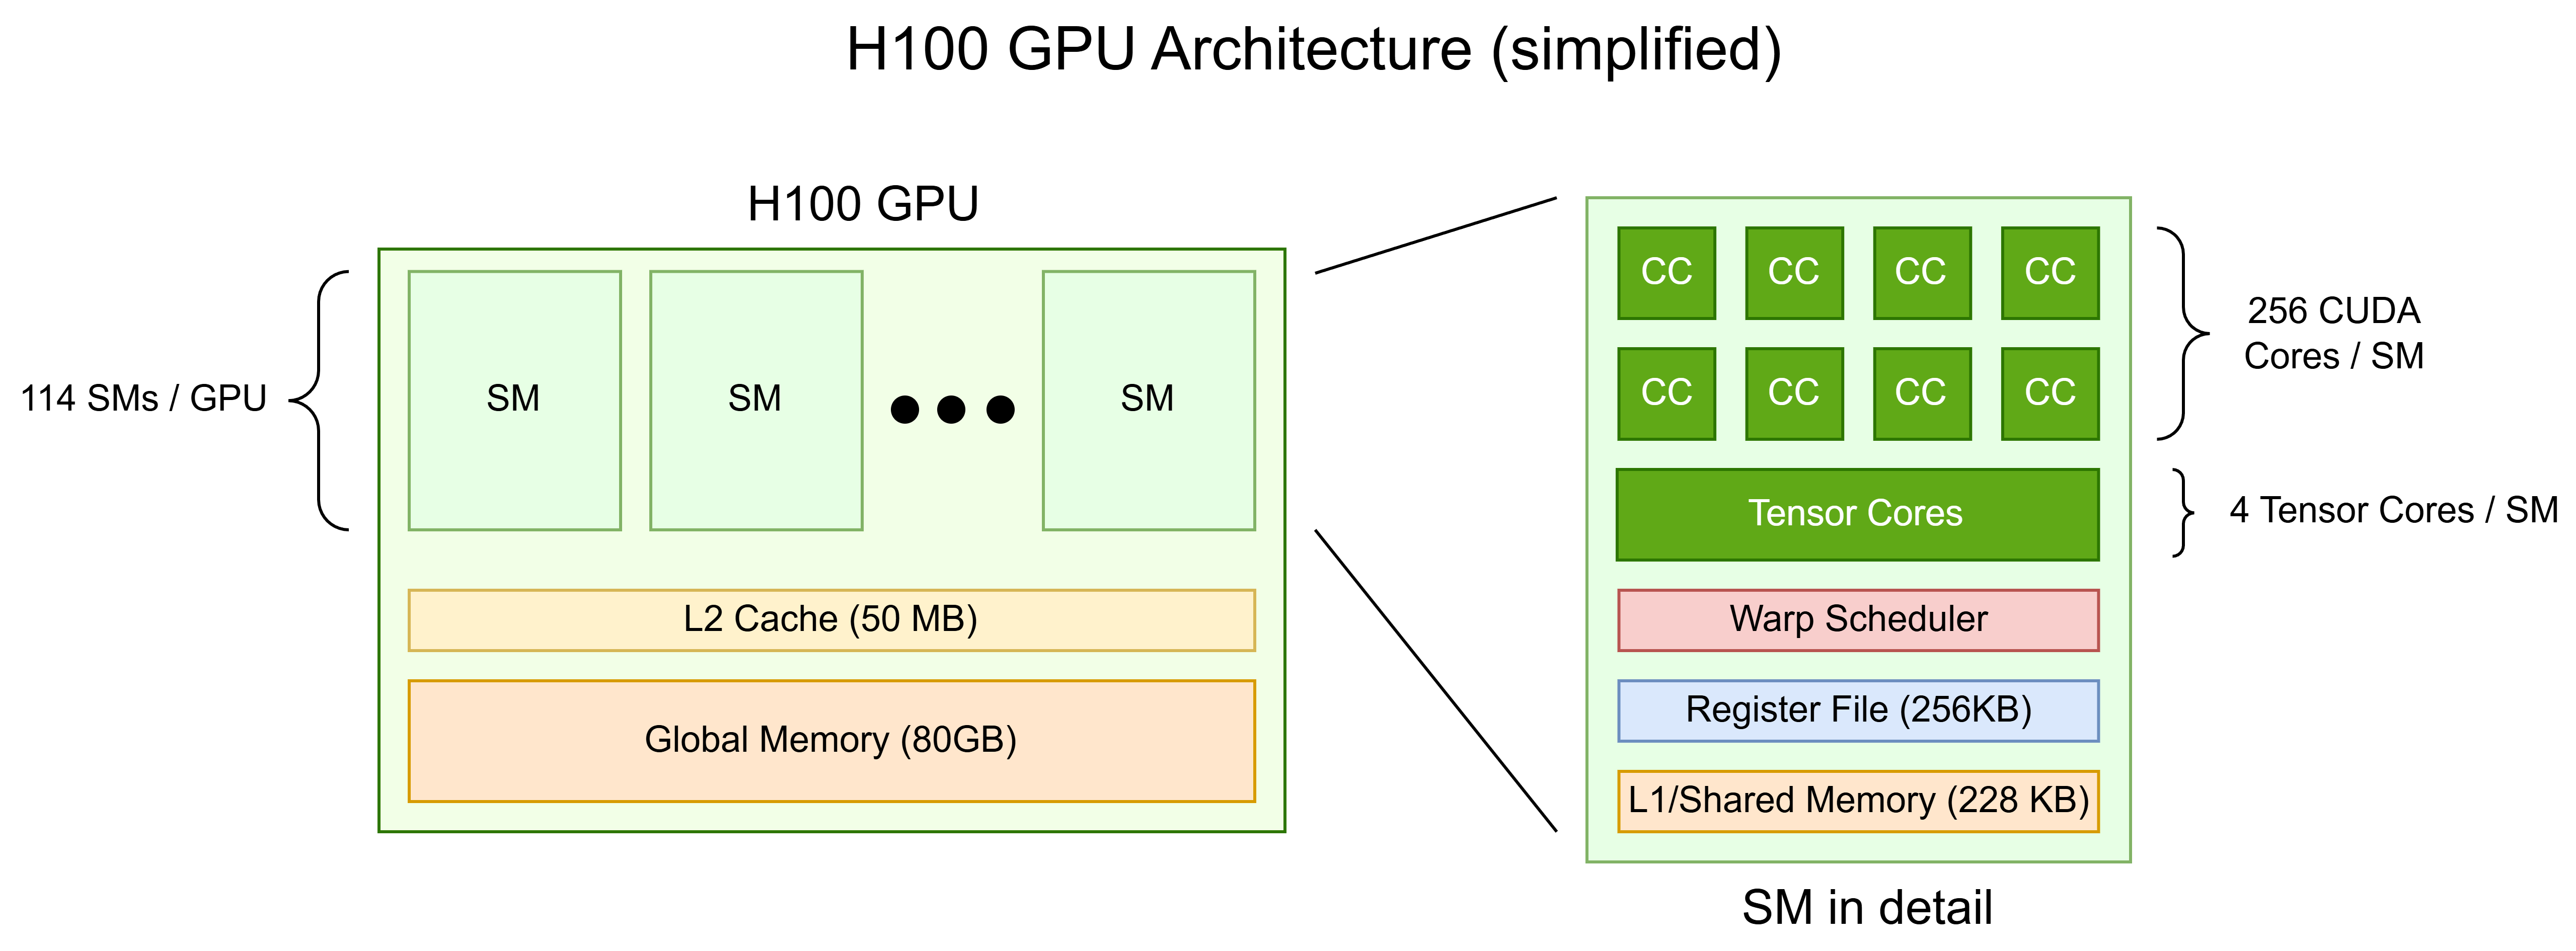
\includegraphics[width=1\linewidth]{figs/diags/gpu_architecture.png}
    \caption{A simplified diagram of the H100 GPU architecture. Although absolute core counts and memory capacities differ between models, the relative proportions of SMs, compute cores, and memory hierarchy are broadly consistent across modern NVIDIA GPUs.}
    \label{fig:gpu-arch}
\end{figure}

% \subsubsection{GPU execution model}

\subsubsection{Programming with CUDA}
\label{sec:cuda}

For ease of development, the CUDA platform abstracts low-level GPU hardware into a high-level programming model. At the core of this model is the \textit{kernel grid}, which executes a set of instructions called a \textit{kernel} across the GPU. A kernel is function that can perform simple tasks such as matrix addition (see Alg.~\ref{alg:matrix_addition}), to more complex ones such as large accumulate/reduce patterns.

A kernel grid is subdivided into \textit{thread blocks}, each containing multiple \textit{threads}. Multiple thread blocks can be executed concurrently on a single SM, though a single thread block cannot span multiple SMs. Threads are executed in lockstep in groups of 32 called \textit{warps} \cite{nvidia_warp_level_2020}. Within a warp, threads are referred to as \textit{lanes} and are indexed from 0 to 31, each with their own independent register state. Each warp issues a single instruction per clock cycle, causing all 32 lanes to advance in lockstep while executing that instruction on the SM’s shared functional units (e.g., CUDA or Tensor Cores). A visual explanation of CUDA threads, blocks and grids is shown in Fig.~\ref{fig:nvidia-cuda-model}.

\begin{algorithm}[H]
	\label{alg:matrix_addition}
	\begin{algorithmic}[1]
		\State \textbf{Inputs}: Matrix $\mathbf{A} \in \Real^{n \times m}$, Matrix $\mathbf{B} \in \Real^{n \times m}$, Matrix $\mathbf{C} \in \Real^{n \times m}$, $m \in \Nat$
		\State \textbf{Define} \textbf{Kernel} \texttt{matrixAdd}($\mathbf{A}$, $\mathbf{B}$, $\mathbf{C}$, $m$):
        \State \quad $i \gets m \times blockIdx.x + threadIdx.x$
		\State \quad $\mathbf{C}[i] \gets \mathbf{A}[i] + \mathbf{B}[i]$
		\State \textbf{End Kernel}
	\end{algorithmic}

    \caption{Matrix addition using CUDA. The kernel is launched with $n$ blocks and $m$ threads per block, aligning with the row and column counts of the input matrices.}
    
\end{algorithm}

\begin{figure}[H]
	\centering
	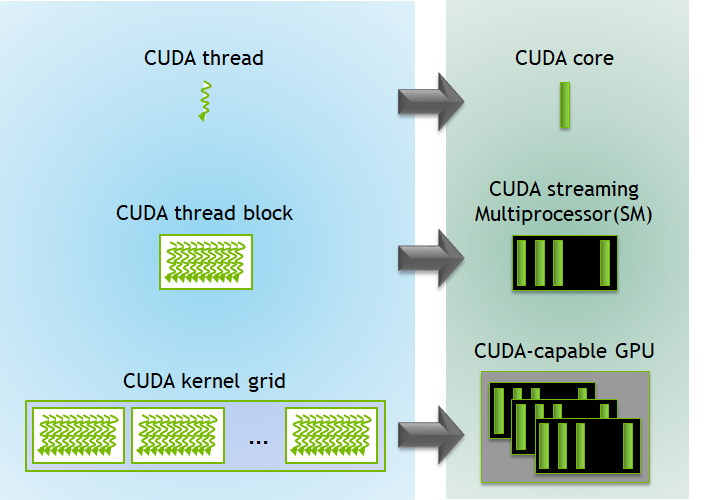
\includegraphics[width=0.6\linewidth]{figs/diags/nvidia-cuda-model}
	\caption{Simplified overview of the CUDA programming model \cite{CUDARefresher2020}}
	\label{fig:nvidia-cuda-model}
\end{figure}

\section{Related Work}

\subsection{Approximate Nearest Neighbour Search}

As discussed in Section \ref{sec:anns}, ANNS is often preferred to exact NNS because of scalability issues with modern large-scale datasets. As a result, ANNS has become a large and rapidly growing research area. Typically, an ANNS method is composed of two stages: \textit{indexing} and \textit{querying}. Indexing constructs a data structure over $X$ that supports fast retrieval, while querying uses this structure to recover the $k$ nearest neighbours of a query $\bq$. Nearly all ANNS query methods rely on a two-stage retrieval strategy: first producing a small candidate set from $X$, then evaluating exact distances within that set to a query $\bq$. Distances may be computed exactly, or approximated using techniques such as vector quantization \cite{ge2013optimized, kalantidis2014locally, douze2025faiss}. Although these methods reduce memory and increase throughput, they fall outside the scope of this work. We therefore assume that the original dataset $X$ is stored explicitly, enabling exact distance evaluation.

Research into ANNS generally attempts to optimise indexing and querying for real world applications of ANNS. Since ANNS is often done on large scale datasets, it is vital that a created algorithm is minimally resource intensive. Ideally, an ANNS algorithm is fast to index and query, has a low memory footprint and is accurate. In large-scale recommendation systems, for example, low latency, high precision, and low memory usage are all critical for economic and operational scalability.

Of particular importance to an ANNS algorithm is the data domain on which it is applied. It is often the case that an algorithm has much better performance on one dataset as compared to another, along a specific trade-off curve (for example, accuracy over queries answered per second) \cite{jaasaari2025vibe,aumuller2020ann}. Consequently, when evaluating the relative performance of an ANNS algorithm to competitors, it is vital to benchmark it on across a wide range of datasets and performance metrics, such as accuracy, query throughput, and index size.

Research into ANNS algorithms can be coarsely divided into four broad families: graph-based methods, inverted file indexing, hashing techniques, and tree-based approaches. Its important to note that these families should be understood primarily as organisational abstractions, grouping methods by their dominant indexing and query mechanisms rather than by shared theoretical guarantees or performance characteristics. In practice, many modern ANNS methods combine elements from multiple families, which makes broad, family-level descriptions of behaviour difficult to justify.

\paragraph{Graph-based indexes.}

Graph based methods \cite{wang2021comprehensive,harwood2016fanng,fu2017fast,malkov2018efficient} generally aim to organise a dataset into a graph structure that is facilitates fast and accurate searching at query time. A common pattern is to use dataset points as nodes within a graph, and to have connecting edges between nodes indicating proximity of the corresponding points. Once an index is created, it can be searched to find a set of candidate neighbourhood points for a query. A key graph-based ANNS algorithm is Hierarchical Navigable Small World Graphs (HNSW) \cite{malkov2018efficient}. HNSW constructs a multi-layer graph in which connections tend to span larger distances in higher layers and progressively shorter distances toward the bottom layer. Querying proceeds via greedy traversal from the top layer until a local minimum is reached, after which the search descends layer by layer, using each local minimum as the entry point for the next layer. At the bottom layer, distances are evaluated for a limited set of candidate points to return the $k$ nearest neighbours. The idea of HNSW's layered graph traversal is shown in Fig.~\ref{fig:hnsw}

\begin{figure}
    \centering
    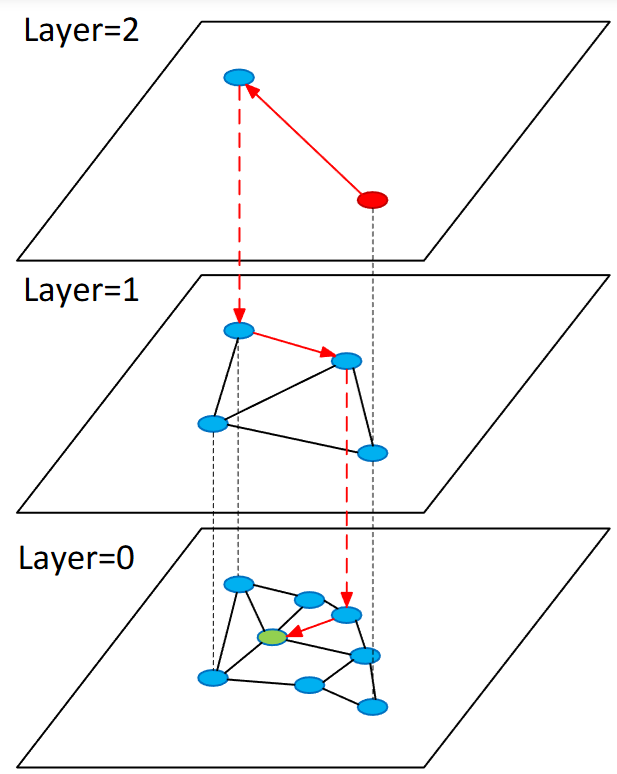
\includegraphics[width=0.3\linewidth]{figs/diags/hnsw.png}
    \caption{Illustration of the HNSW search process \cite{malkov2018efficient}. The search starts from the red entry point and greedily traverses the hierarchy, descending layer by layer until reaching a neighbourhood of points near the query $\bq$ (shaded green).}
    \label{fig:hnsw}
\end{figure}

\paragraph{Inverted file indexing.}

Another key ANNS family utilizes Inverted File Indexing (IVF) \cite{baranchuk2018revisiting,amato2014mi,amato2008approximate,douze2025faiss}. This creates an indexing structure that is essentially an coarse partitioning of the dataset into \emph{clusters} (also known as \emph{cells}). Each dataset vector is assigned to a single cluster defined by a coarse partition of the vector space. This partition is typically learned during index construction, for example using k-means, and vectors are assigned via nearest-cluster matching. At the query stage, clusters are selected according to the proximity of their centroids to the query, and the vectors within these clusters make up the candidate set for a query. Since IVF indices are essentially a re-ordering of a dataset, they have a minimal memory footprint. Additionally, since clusters can be stored contiguously in memory, this allows IVF algorithms to be relatively cache efficient to other ANNS algorithms. The FAISS library \cite{douze2025faiss} is a NNS library that implements several IVF based methods. Of note is the 'IndexIVF' index type \cite{faiss_indexes_wiki}, here, the number of clusters is dictated by the parameter $nlist$. When querying, the vectors in the nearest $nprobe$ cells are searched to perform distance computations over. While FAISS's IndexIVF was originally built for CPUs, they provide a GPU implementation which will be discussed further in Sec.~\ref{sec:gpuAnns}. An illustration of IVF indexing and querying for ANNS is shown in Fig.~\ref{fig:ivf}.

\begin{figure}
    \centering
    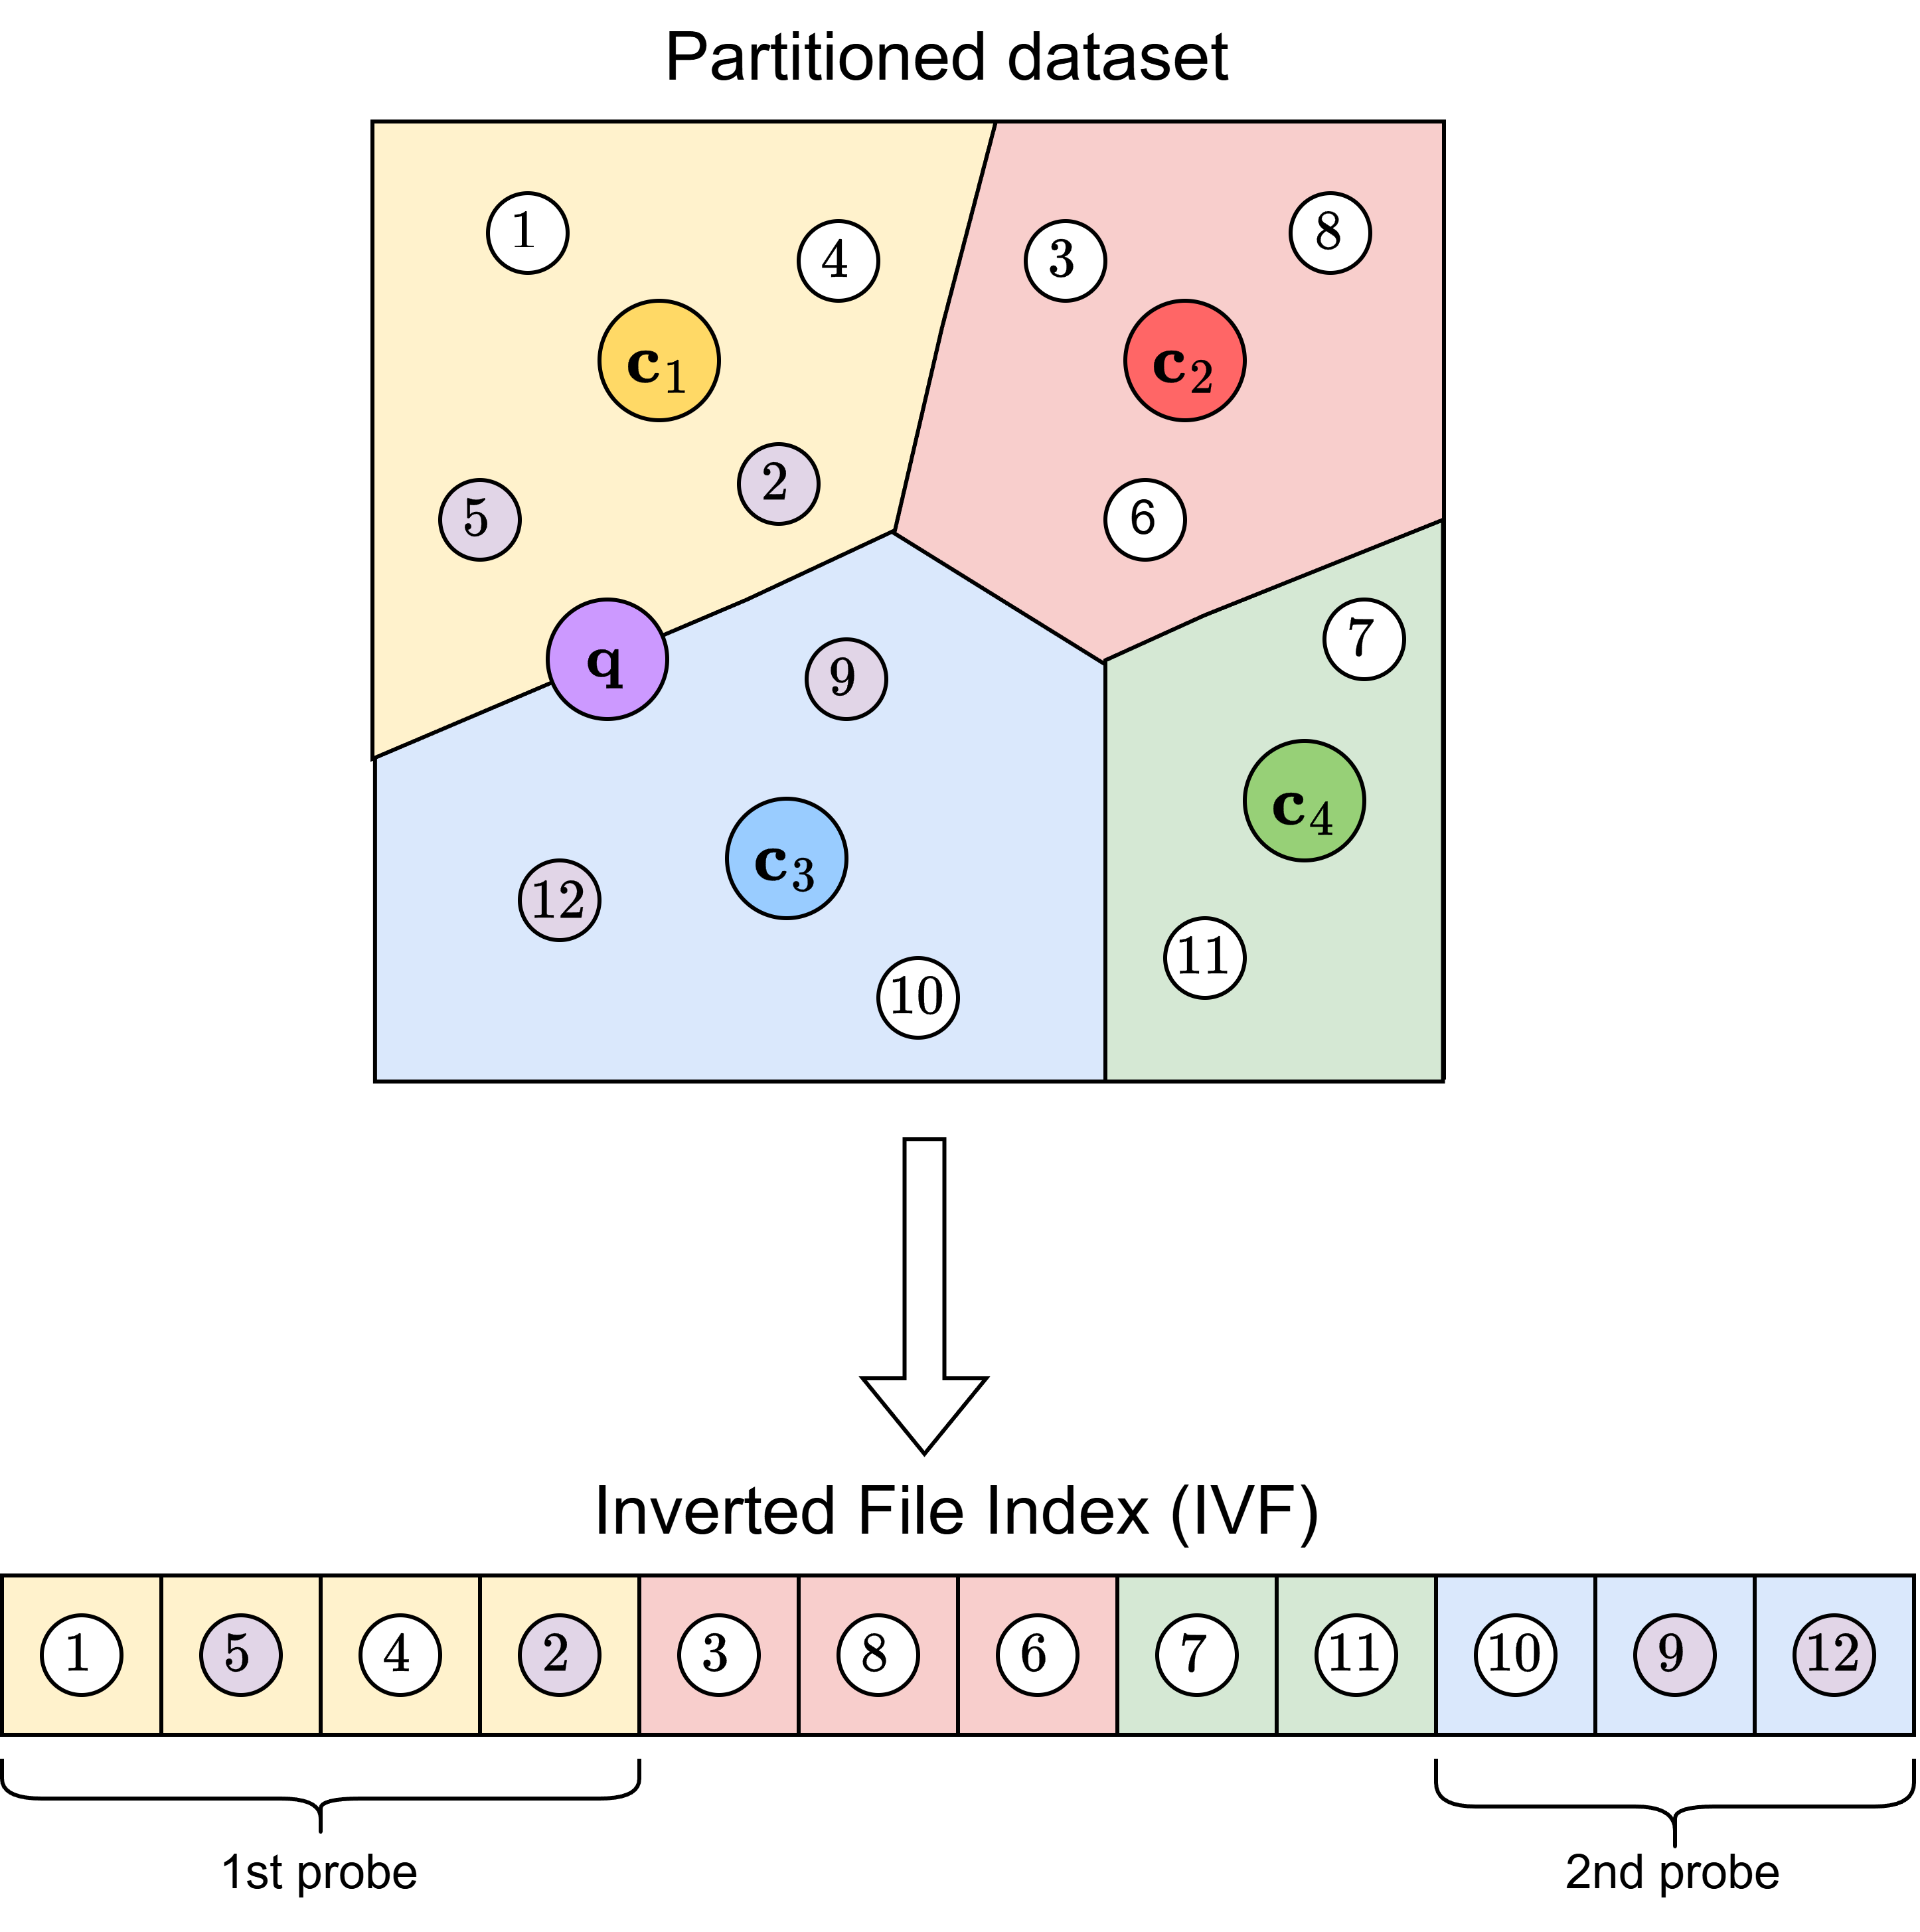
\includegraphics[width=0.5\linewidth]{figs/diags/faiss-ivf.png}
    \caption{Illustration of IVF partitioning and indexing on a dataset $X$ with $nlist=4$. During querying, a top-$k$ ANNS query is performed for $\bq$ with $k=4$. With $nprobe=2$, the partitions associated with centroids $\mathbf{c}_1$ and $\mathbf{c}_3$ are searched, and exact distances are evaluated within these partitions. The resulting nearest neighbours are the points labelled $2, 5, 9,$ and $12$.}
    \label{fig:ivf}
\end{figure}

\paragraph{Hashing methods.}

Other key algorithms are based on hashing techniques \cite{pham2022falconn++,pham2021simple,cheng2024robust,pan2011fast,becker2016new}. These use randomized hashing functions to add dataset points to a \emph{buckets}. This is done such that nearby dataset points are likely to be stored in the same buckets, while disparate points aren't. To find the neighbours to a query, the hash functions are used to find the closest buckets to a query, the intersection of these buckets then form the candidate set to perform distance calculations over. Hashing functions are often fast to execute, often relying on relatively fast techniques such as random projections, bitwise operations and Fast Hadamard Transforms \cite{jafari2021survey, pham2022falconn++}. However, this speed often comes at the expense of query accuracy, consequently it is often necessary to add dataset points to multiple buckets \cite{xu2011complementary,lv2007multi}, which improves query accuracy at the expense of larger indices. A key sub-category of Locality Sensitive Hashing (see Sec.~\ref{sec:lsh}), used by algorithms such as FALCONN \cite{andoni2015practical}, ACHash/DHHash \cite{dasgupta2011fast}, SRP-LSH \cite{ji2012super} and others \cite{pan2011fast,gorisse2011locality,huang2015query,wang2014hashing,jafari2021survey}. Other sub-categories include Spectral Hashing \cite{weiss2008spectral}, and Semantic Hashing \cite{salakhutdinov2009semantic}. 

\alert{Mention LSF here - this is a blindspot!}

\paragraph{Tree based indices.}

Another important family of methods uses tree-based indices \cite{hyvonen2016fast, jaasaari2019efficient, ram2019revisiting, sun2023soar, bernhardsson2015annoy}, in which the dataset is partitioned using tree-like structures. At query time, the created tree index can be traversed to find a set of candidate points for a query. A key tree based algorithm is Spotify's ANNOY \cite{bernhardsson2015annoy}. This repeatedly subdivides the dataset into subdivisions defined by random hyperplanes between sampled points (see Fig.~\ref{fig:annoy}. Others approaches use $kd$-trees \cite{ram2019revisiting,chen2019fast,panigrahy2008improved}, which repeatedly splits a $k$ dimensional dataset across one dimensional hyperplanes to construct a tree. $kd$-trees are not naturally suited to large scale datasets \cite{panigrahy2008improved}, thus a small body of research is focussed utilizing $kd$-tree based techniques for large scale datasets \cite{panigrahy2008improved,avrithis2016high,ram2019revisiting}.

\begin{figure}
    \centering
    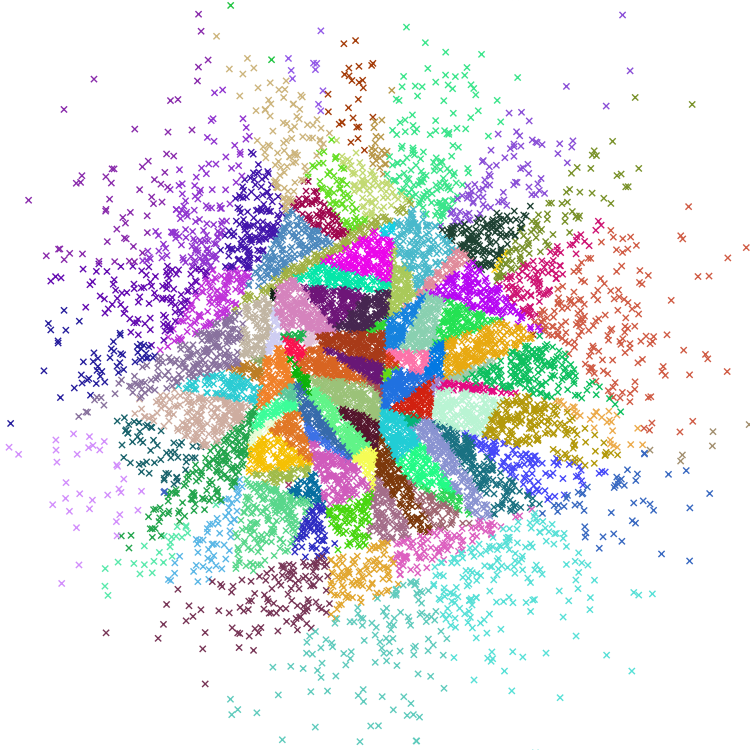
\includegraphics[width=0.5\linewidth]{figs/diags/annoy.png}
    \caption{Graphical illustration \cite{bernhardsson2015annoy} of ANNOY’s recursive space partitioning, where each shaded region corresponds to a node in the search tree. Queries traverse this structure to identify a subset of candidate points for distance evaluation.}
    \label{fig:annoy}
\end{figure}

\subsection{GPU Accelerated Nearest Neighbour Search}
\label{sec:gpuAnns}

While research into nearest-neighbour search (NNS) has traditionally focused on CPU-based algorithms, a parallel line of work explores the use of GPUs to accelerate NNS. As discussed in Section \ref{sec:gpus}, GPUs are particularly well suited to arithmetic-heavy and highly parallel workloads, making them a natural fit for both exact and approximate NNS. In practice, queries are typically processed in large batches—often hundreds or thousands at a time—to maximise resource utilization. Since individual queries can be evaluated largely independently, this batch structure maps cleanly onto the GPU’s parallel execution model. Moreover, a dominant computational bottleneck in many ANNS methods is the evaluation of large numbers of independent distance computations between a query and its candidate points, a task that GPUs are especially effective at accelerating.

Early GPU NNS methods focused on computing exact NNS. A foundational from Garcia et al.\ (2018) implemented a brute force NNS algorithm using the CUDA platform \cite{garcia2008fast}. This was shown to be orders of a magnitude faster than existing CPU brute force methods, creating the groundwork for future methods using GPUs to accelerate NNS. However, owing to the same reasons of necessity and practicality that limit exact NNS (see Sec.~\ref{sec:anns}), GPU-based NNS research has largely focused on ANNS. Also, much like CPU ANNS, GPU ANNS algorithms can be largely grouped into families of approach.

\paragraph{GPUs graph-based indexes.}
Perhaps the largest subfield of GPU ANNS is the use of graph based methods \cite{groh2022ggnn,zhao2020song,harwood2016fanng,sun2022out,yu2022gpu,ootomo2024cagra,li2025scalable}. SONG (2020) \cite{zhao2020song} is a graph searching algorithm built using a GPU for executing queries in an accelerated manner. It relies on a myriad of techniques such as hashing tables and memory optimizations to greately accelerate graph searching over traditional graph based CPU ANNS methods. However, a key weakness is that it relies on a prebuilt graph index (e.g. A NSW graph \cite{malkov2014approximate} using a CPU), consequently, it doesn't offer accelerated methods to create the necessary index it requires. On the other hand, GGNN (2022) \cite{groh2022ggnn} provides a fully GPU-accelerated pipeline for both index construction and querying, although graph construction can remain computationally expensive. FANNG \cite{harwood2016fanng} exploits assumptions about low intrinsic dimensionality to construct a graph index that is searchable on either CPU or GPU, but this reliance on data distribution properties - specifically for feature vector datasets - limits its general applicability across other datasets.

\alert{MENTION Cagra! \cite{ootomo2024cagra}}

\paragraph{GPU IVF methods.}

Perhaps the most well-known GPU ANNS methods are provided by the FAISS library \cite{douze2025faiss}. FAISS implements a broad range of GPU-accelerated index types, including exact search, inverted file indexing (IVF), and quantization-based methods such as Product Quantization (PQ) \cite{kim1999quantization}. While PQ-based indices are central to large-scale ANNS due to their memory–accuracy trade-offs, they rely on approximate distance evaluations and are therefore less relevant in this context. Among FAISS’s offerings, GpuIndexIVFFlat, which performs ANNS using exact distance computations, is the most relevant point of comparison with CuFalconn. Independent of the specific index type, FAISS is a natural comparison point due to the maturity and generality of its GPU ANNS implementation. The underlying IVF methodology is well studied and has demonstrated robust performance across a wide range of datasets in CPU-based evaluations \cite{aumuller2020ann, jaasaari2025vibe}, suggesting similar breadth of applicability when deployed on the GPU. Coupled with a long development history and sustained optimization effort, FAISS can reasonably be regarded as a current state-of-the-art reference for GPU-based ANNS.

\paragraph{Hashing and tree methods.}

Besides graph based methods and FAISS, there have been a handful of other approaches to accelerate ANNS using a GPU. Wieschollek et al.\ \cite{wieschollek2016efficient}, used PQ \cite{kim1999quantization} to create searchable trees called Product Quantization Trees (PQT) on the GPU. An LSH-based approach, FLASH \cite{wang2018randomized}, was designed for ultra-high-dimensional datasets, where both the dataset size and dimensionality are high ($n$ large and $n \approx d$). While FLASH demonstrates substantial speedups in this regime, its effectiveness on more conventional datasets - where $d \ll n$ - remains yet unproven.

\paragraph{Hybrid and Multi-GPU.}
Beyond the conventional use of a single GPU for ANNS acceleration, several works explore more unconventional GPU utilization strategies. Hybrid CPU–GPU approaches explicitly partition computation across hardware units to balance memory constraints and computational efficiency \cite{xiang2019accelerating,tian2024fusionanns}. For instance, GAIPS \cite{xiang2019accelerating} performs aggressive pruning and quantized scoring on the GPU, while delegating final exact inner-product evaluation to the CPU when datasets exceed GPU memory capacity. On the other hand, algorithms designed for cooperative multi-GPU workloads target scalability at industrial scale, distributing data or computation across devices to handle massive datasets \cite{johnson2019billion,kato2012multi,groh2022ggnn}.

% \subsubsection{CSR Bucket Format}

% As discussed above, buckets from all repeats are stored contiguously in GPU memory in a CSR format. This is done so that the bucket index is easy to handle with GPU libraries and kernels which are heavily based on number-based indexing of contiguously stored data structures. This is composed of three arrays: $buckets$, $starts$ and $sizes$. $buckets$ has a length equal to the total number of points in all buckets after the CPU max-heap keeps only the top points per bucket. Conversely $starts$ and $sizes$ both have fixed lengths $L \cdot 4D^2$.

% Take an bucket with index $\tau = i \cdot 4D^2 + j$, where $i$ is the repeat index, and $j$ is the local index of a bucket within a repeat. The start index and size of the $\tau$th bucket are thus $starts[\tau]$ and $sizes[\tau]$ respectively. The contents of this bucket are then stored at:

% \begin{equation}
%     buckets[starts[\tau]], buckets[starts[\tau]+1], buckets[starts[\tau]+2] \dots buckets[starts[\tau]+sizes[\tau]-1]
% \end{equation}

% \begin{table}[]
%     \centering
%     \begin{tabular}{c|c}
%          $m$ & max bucket size  \\
%          $D$ & number of random projections for the $U$ and $V$ matrices \\
%          $p$ & the number of probes per dataset point, per repeat \\ 
%          $L$ & the number of hash tables (repeats) to perform
%     \end{tabular}
%     \caption{Indexing parameters for \cf. For brevity, we use slightly different naming convention to the original \fpp paper}
%     \label{tab:placeholder}
% \end{table}

\section{CuFalconn}

\cf is a GPU-accelerated adaptation of \fpp. It implements largely the same processes; however, several key modifications are introduced to better align with GPU execution constraints. In this section, we will briefly motivate why we choose to adapt \fpp for the GPU. Before describing how \cf is practically implemented in the indexing and querying stages. Additionally, whereas \fpp only supported angular distance, we describe the natural progression allowing \cf to accomodate both angular and inner product distance.

\subsubsection{Motivating \cf}

Besides the well established success of numerous GPU accelerated ANNS methods, we highlight two key reasons supporting the suitability of \fpp for GPU acceleration. Firstly, Pham et al. demonstrated that \fpp achieves superior query performance compared to baseline Falconn implementations at equivalent indexing space. This is notable because Falconn is derived from an LSH family with asymptotically optimal indexing space, characterised by $\rho \approx 1/c^2$ for \crNN. Despite this theoretical optimality, \fpp delivers stronger practical performance on the more relevant $k$ANNS task while operating under the same memory budget. Consequently, within the broader family of LSH based ANNS algorithms, \fpp's memory efficiency makes it a strong candidate for GPU acceleration, where memory comes at a premium compared to CPUs. 

Secondly, \fpp presents substantial opportunities for parallel processing, particularly in inner product computations underpinning both hashing and distance evaluation. While inner products define the hashing mechanism (e.g., $\dotxr$ during indexing and $\dotqr$ during querying), the dominant computational burden during querying arises from finding $\dotqr$ for each candite of a query. Pham et al. showed that these distance computations are the deciding factor in querying speed \cite{pham2022falconn++}. The large collections of independent inner products required for hashing and distances can be expressed as matrix multiplications, a workload pattern for which GPUs excel in relative to CPUs~\cite{huang2019gpu}. In addition, query-level parallelism is inherent: queries within a batch are independent and can therefore be executed concurrently, further aligning \fpp with GPU execution models.

\subsection{\cf Indexing}

The indexing process of \cf is a \emph{hybrid} CPU and GPU approach, whereby both of these processors are used. It follows largely the same indexing process as \fpp - meaning it constructs an LSF inspired index using $L$ repeats of the Falconn hashing process using a $l=2$ layer hash function. There are however, a few key nuances of \cf that make it more than just accelerating \fpp with a GPU. 

The main difference between \cf and \fpp indexing is that we remove the bucket scaling parameter $\alpha$. Instead we set a maximum bucket size by keeping the at most the top-$m$ scoring points per bucket. This has several advantages. Firstly, $m$ is more interpretable than $\alpha$. In the original \fpp formulation, $\alpha$ is tested with small fractional values (e.g., $0.1$ or $0.01$), whose practical effect on bucket occupancy is indirect. By contrast, $m$ directly specifies the maximum number of points per bucket, providing clearer control. Secondly, a fixed bucket size $m$ permits selecting values that are well suited to GPU execution, such as powers of two. While CUDA does not require power-of-two dimensions, such choices often improve warp-level efficiency and simplify scheduling. For example, when gathering candidates from buckets, setting $m=8$ allows a single warp (32 threads) to process $32/8 = 4$ buckets concurrently, increasing compute and memory throughput. 

\cf uses a hybrid CPU-GPU process to simplify the process of filling buckets with points. While most of indexing is completed on the GPU, the actual process to probe and rank points into buckets is done fully on the CPU. This is done by implementing each bucket as a size-$m$ CPU heap. Data transfers between the CPU and GPU are done using \emph{pinned} memory, which can significantly increase in-memory transfers in both directions \cite{pytorch_pinmem_nonblock}. This choice also simplifies the algorithm: a CPU-resident bounded heap provides a direct and reliable mechanism for enforcing the per-bucket top-$m$ constraint, while avoiding the additional complexity introduced by highly irregular and contention-heavy per-bucket updates on the GPU. Although a fully GPU-resident alternative (e.g. segmented top-$m$ selection) is feasible, it would reasonably require intricate synchronisation patterns and memory management. We therefore leave a completely GPU-resident implementation of \cf as future work. 

Since GPUs are primarily designed for operations based on accessing large scale arrays and tensors, \cf is implemented with this in mind. To this end we can re-express the dataset $X = \{ \bx_1, \bx_2, \dots, \bx_n \}$ as a $n \times d$ tensor $\bX$, where a point $\bx_i \in X$ is stored \emph{row-major} order along the $i$th row. We store the sets of random vectors $R$ and $S$ across \emph{all} $L$ table repeats into two tensors, $\bR, \bS \subset \Real^{L \times d \times D}$. For a repeat $i \in [L]$, the sub-tensors $\bR_i, \bS_i \subset \Real^{d \times D}$ contain the sets of random vectors for this repeat stored in \emph{column-major} order. The re-expressing of $X, R$ and $S$ simplifies finding random projections between data points and random vectors into a matrix multiplication - an operation that a GPU is well optimised for. The pseudo code in Alg.~\ref{alg:cfIndexing} outlines the indexing process of \cf.

\alert{Talk to Ninh. about this - do we need to talk about CSR format.}

\alert{
Points to comment on:
Buckets stored concurrently in CSR across all buckets. 
Only point indices are stored in buckets. 
Use matrix multiplication for X prime tensors (tensor library)
}

\alert{We should justify why we use a for-loop for repeats: the memory constraints are particulary high otherwise.}

\begin{algorithm}
	\caption{\cf Indexing}
	\label{alg:cfIndexing} 									
	\begin{algorithmic}[1]
		\Procedure{Indexing}{$\bX$, $\bR$, $\bS$, $L$, $\ip$, $m$}
            \State Centre dataset: $\bX \gets \bX - \bx_c$ \Comment{Row-wise broadcast}

            \\
            
            \For{For $L$ repeats}
                \State $\bXpR \gets \bX\bR$ \Comment{Matrix multiplication} 
                \State $\bXpS \gets \bX\bS$
                
                \\
                
                \State Combining directions from $\bXpR$ and $\bXpS$, find the top-$iProbes$ buckets to probe for each point in $\bX$
                \State Copy the indices of the top buckets found per data point into a CPU tensor $\bP \in \Nat^{n \times \ip}$

                \\

                \For{$i \gets 1$ \textbf{to} $n$ \textbf{in parallel on CPU}}
                    \For{$j \gets 1$ \textbf{to} $\ip$}
                        \State Insert $\bx_i$ into the size-$m$ min-heap of bucket indexed by $\bP[i,j]$ in CPU memory
                    \EndFor
                \EndFor

                \State

                \State Copy contents of all buckets from CPU to GPU memory in a flattened format
                
            \EndFor
		\EndProcedure
	\end{algorithmic}
\end{algorithm}

\subsection{\cf Querying}

As compared to indexing, \cf querying is done \emph{entirely} on the GPU. Much like \fpp, the querying process is decomposed into a few key stages: hash query to find the nearest buckets, gather candidates from these buckets, then perform distance computations of these candidates to find the closest points.

The hashing process of querying is largely the same as \fpp, for two sets of random vectors, we find the top scoring buckets to provide candidate points. However, the selection process is slightly different. To narrow the search of the top buckets for each query, we only consider the top-$topDirs$ directions per layer per repeat, then combine these to attain a selection of the $topDirs^2$ buckets per repeat. To then find the $\qp$ closest buckets to a query, we limit our search to the $L \cdot topDirs^2$ gathered buckets across all repeats. Heuristically, we set $topDirs = \lceil \sqrt{\qp / L} \lceil$, this ensures $qProbes \leq L \cdot topDirs^2$, such that there is atleast $\qp$ buckets gathered. This was mainly done for the interests of practicality. Finding \emph{exactly} the nearest buckets to a query out of all $L \cdot 4D^2$ buckets, would require the computation of a large pair-wise sums of all bucket scores across all repeats, a process that scales with the square of $D$ - for large $D$ this is can take a non-trivial amount of time, even for a modern GPU. Limiting our search to the combinations of top-$topDirs$ directions per layer per repeat narrows this search greatly. For a typical indexing and querying configuration of \cf (see Sec.\ref{sec:experiment}), $topDirs^2 \ll 4D^2$, so far fewer pair-wise sum need be computed. Strictly speaking, this heuristic may miss out on nearby buckets to $\bq$ - consider the case where a bucket not formed by the $topDirs^2$ considered in a repeat is still one of the top-$qProbes$ buckets across all repeats. However, for $L$ large enough, this effect can be mitigated, as missed candidates in a passed bucket of one repeat can instead be found in another repeat. 

\alert{Need to give a more proper idea of what values $topDirs$ could take - e.g. take some typical values, and show what they are.}

\alert{This last sentence is a little imprecise. }

Besides this added nuance of selecting the closest buckets to a query, the querying process of \cf is functionally the same as \fpp. However, of course, it is implemented to use a GPU instead of a CPU. 

The collection of candidates for a query is done using a custom CUDA kernel. Essentially, this uses the indices of the closest buckets to perform a scattered-gather pattern of the indices of all points within the closest buckets. Using a small max bucket size $m$ that \emph{divides} 32 is advantageous to performance. As this allows one warp to collect candidates across $32/m$ buckets simultaneously. Which in-turn increases the occupancy of the GPU - resulting in better performance. A \emph{variable} max bucket size introduced by the scaling parameter $\alpha$ of \fpp, would be more computationally intensive - requiring more pre-processing and data-staging before launching a gather kernel. Besides decreasing index memory size, this is another benefit of using a fixed bucket size.  

\alert{We need to discuss how distances are found - mention that use a custom function to do distance computations - just say that this is basically just doing IPs over and over again - works for angular distance fi vectors are prenormed}

For a batch of queries, inner products are stored into a large flat jagged array. Where for a query $q$ with a variable $n_c$ number of candidates, the inner products with it's query are stored in a segment of $n_c$ length. The top-$k$ candidates for each query are selected using a top-$k$ select kernel which is a modification of FAISS-GPU's \cite{johnson2019billion} \ws. \ws was modified such that it could easily handle top-$k$ inner product selection over variable length segments for the inner products with queries with each of their candidates. The top-$k$ candidates per query are then returned to answer $k$ANNS.

\alert{re-write the above. Perhaps some more elaboration - why did we choose the top-$k$ select from FAISS - say its demonstrably very fast}. 

\alert{Explain further on this kernel. Take alternative approaches, and then explain why they don't work. There are essentially two: large scale data staging before hand. Although I'm not totally sure why this is better, yes better data staging. But I'm struggling to come up with words to make it plain for the reader. And a tiling inner products kernel - we tried this and it didn't work!}


% A key thing to note is that candidate vectors are fetched essentially in a random scattered order - this is incongruent with modern GPU patterns for performing large scale multiply-reduce patterns. Ideally, candidate vectors would be staged continuously into large arrays, this could then allow a


% . Staging all candidate vectors for each query would require large, variable-sized intermediate arrays, which is both memory-intensive and unscalable for large datasets. As a result, the computation operates directly on gathered data vectors, preventing the use of dense, block-structured execution patterns and accelerated workflows such as tensor-core-based matrix operations.

As is common with ANNS applications, we assume that a queries are processed in batches. To this end consider a collection of $n_q$ queries stored in a tensor $\bQ \in \Real^{n_q \times d}$, where queries are stored in row-major order. 

\begin{algorithm}
	\caption{\cf Querying (GPU)}
	\label{alg:cfQuerying} 									
	\begin{algorithmic}[1]
		\Procedure{Querying}{$\bX, \bQ, \bR, \bS, L, \qp, topDirs, k$}

            \\ 
            \State Project $\bQ$ onto vectors in $\bR$ and $\bS$ across all repeats

            \\ 
            \State For each query, select top-$topDirs$ directions from $\bR$ and $\bS$ per repeat
            \State Combine the top-$topDirs$ directions per repeat and find their scores
            \State For each query find the top-$\qp$ buckets out $L \cdot topDirs^2$ prospective buckets
            \\ 
            \State Collect candidates indices from selected buckets for each query

            \\
            \State Use candidate indices to find inner products between each query in $\bQ$ and candidates in $\bX$

            \\
            \State Select top-$k$ candidates per query using modified \ws kernel

            \State \Return top-$k$ nearest neighbours

		\EndProcedure
	\end{algorithmic}
\end{algorithm}

\subsection{Extension to inner product distance}

The original \fpp was designed for angular distance, where similarity is maximised via inner products on the unit sphere. We extend \cf to support inner product distance directly. This extension is inspired by the \textit{CEOs} family of algorithms \cite{pham2021simple}, which are largely built on the CEOs property in \ref{sec:ceos} for inner product distance.

At a high level, \textit{CEOs} indexing consists of projecting dataset point onto a set of Gaussian random directions and storing the top-$m$ dataset points per projection direction. Querying follows an analogous pattern: the query is projected onto the same directions, the top-$s$ directions are selected, and a candidate set is formed from the union of the stored top-ranked points associated with these directions. A practical limitation of this approach is that achieving strong retrieval performance typically requires very large indices.

\cf bears strong resemblance to this general strategy and may be viewed as a simplified variant. Instead of storing the global top-$m$ vectors for every projection direction, each direction retains only points for which it is among their top-$iProbes$ most significant directions. This modification substantially reduces indexing space,while preserving excellent querying performance. For example, to attain high query accuracy on the GIST dataset, \textit{CEOs} requires index sizes on the order of GBs, while \cf can achieve similar results with a few MBs (see Tab.~\ref{tab:gist-imagenet-indexing} in \hyperref[sec:experiment]{Experiment}). 

\alert{Write something how we can denote IP distance as simply the inverse of MIPS, hence the same notation works for the distance function in the preliminary}

\section{Experiment}
\label{sec:experiment}

\alert{Make the experiment better to read at a glance. I.e. update figures/tables etc so marker can see briefly the results}

\alert{A key goal of the experimentation is to tie it back to the theory - make thematic links throughout experiment linking results to what you'd expect from theory.}

\cf is evaluated over several real-world datasets to prove its practical applicability for the $k$ANNS problem. We analyse its its performance for both querying and indexing against competitor algorithms. Consequently, we daw these key conclusions from experimentation:

\begin{enumerate}
    \item \cf offers competitive querying performance against the current state-of-the-art GPU based FAISS library
    \item \cf is faster for both indexing and querying than an equivalent CPU implementation. Indicating that it successfully uses a GPU to accelerate solving the $k$ANNS problem.
\end{enumerate}

\alert{Another conclusion here?}

\paragraph{Implementation details.} 

\cf is written in C++/CUDA and compiled with g++ using the \textbf{-03} optimisation flag. The LibTorch \cite{Ansel_PyTorch_2_Faster_2024} library is used to implement tensor operations. GPU components are executed on an NVIDIA GeForce RTX3090 GPU \cite{nvidia_rtx_3090}, and CPU parts with an AMD Ryzen Threadripper 3970X 2.2.GHz 32-core processor (64 threads) with 128GB of DRAM. \cf uses 64 CPU threads for indexing, enabled with \textbf{\#pragma omp parallel} on $\operatorname{\textbf{for}}$ loops.

\paragraph{Datasets.} 

We choose 4 large dimensional datasets for evaluation: GIST, ImageNet, Yahoo-minilm and Glove-100. Each dataset has an accompanying set of queries for evaluating query performance. For GloVe-100 and ImageNet we randomly select 1000 queries from the dataset, likewise for GIST, but with 10,000 chosen. 
With Yahoo-minilm, we use the set of 10,000 queries provided by VIBE \cite{jaasaari2025vibe}. For angular distance, we transform dataset points to have unit norm. Table.~\ref{tab:datasets} provides detailed information on the datasets chosen.

\paragraph{Competitor algorithms.} 

We compare \cf to two rival algorithms. The first is the IVF based GpuIndexIVFFlat index type from the FAISS GPU \cite{douze2025faiss} library. We do not compare to other FAISS index types including GpuIndexFlatIP because this is for an exact Nearest Neighbour Search, nor do we compare to GpuIndexIVFPQ because this uses vector quantisation to find non-exact distances between queries and candidates. For brevity, in this section, we refer to the GpuIndexFlatIP FAISS implementation as simply \fgpu. \fgpu was chosen as its arguably the SOTA for GPU accelerated $k$ANNS. It has excellent index build times and memory usage, along with robust querying performance on a variety of datasets. The second baseline is \mfpp, a variant of the CPU based \fpp with a fixed max bucket size of $m$ instead of using a scaling parameter $\alpha$ \cite{CEOs_GitHub}. This serves as a reference point for evaluating \cf against a CPU counterpart. We run \mfpp with 64 threads.

\paragraph{Evaluation.} 

We evaluate the indexing and querying performance of the algorithms using several metrics. For indexing we report the index build time and size in memory including the dataset. For querying we report the average queries completed per second (QPS) and recall compared to the ground truth over at-least $5$ trials. All experiments use $k=10$, thus recall is reported using $R@10$. To reflect practical ANNS usage, evaluation is restricted to index and querying configurations on \emph{high-recall} regimes ($R@10 \geq 0.75$). We round all recall values to $3$ decimal places. 

\begin{table}[]
    \centering
    \begin{tabular}{c|c|c|c|c|c}
         Name & $n$ & $n_q$ & $d$ & Size (GB) & Metric  \\
         \hline
         \gist \cite{jegou2010product} & 1,000,000 & 10,000 & 960 & 3.58 & IP \\ 
         \imgnt \cite{ILSVRC15} & 2,340,373 & 200  & 150 & 1.31 & IP \\
         \glv \cite{jegou2010product} & 1,183,514 & 1,000 & 100 & 0.44 & Angular \\ 
         \ymlm \cite{jaasaari2025vibe} & 677,305 & 10,000 & 384 & 0.97 & Angular
    \end{tabular}
    \caption{Chosen datasets for experiments}
    \label{tab:datasets}
\end{table}

\subsection{Performance of \cf on Chosen Datasets}
\label{sec:dataset-perf}

Like most $k$ANNS algorithms, the performance and practical applicability of \cf varies across different datasets. For some datasets, it has very strong indexing and querying performance, but its gains are less pronounced on others. We report the recall vs QPS curve of \cf on all datasets in Fig.~\ref{fig:query-perf}. This is a common method of evaluating $k$ANNS querying performance \cite{aumuller2020ann, jaasaari2025vibe}. Up and to the right is better. 

\subsubsection{Parameter Settings} On all datasets, for simplicity of analysis, we set $m=8$, $iProbes=4$. Other wise we detaiZl the specific indexing parameters for each dataset below:

\begin{itemize}
    \item \textbf{GIST}: Set $L = D = 16$, and select $qProbes$ from powers of two between $8$ and $256$
    \item \textbf{ImageNet}: Set $L = D = 64$  and $L=128, D=128$ respectively, and take $qProbes$ from powers of two between 8 and 32768.
    \item \textbf{\glv and \ymlm}: All combinations of $D$ and $L$ from the set $\{128, 192, 256, 392\}$. We then choose $qProbes$ from all powers of two between $8$ and $32768$.
\end{itemize}

The choice of parameters for each dataset was motivated by the corresponding performance of \cf compared to \fgpu (see Sec.~\ref{sec:faiss-compare}). For GIST and \imgnt, we found that we could set $L$ and $D$ relatively small, and still get excellent results compared to \fgpu. On GIST we found we could use smaller $qProbes$ than on ImageNet and still achieve near perfect recall. On \glv and \ymlm we elected to do a sweep of combinations of $(D, L)$ to have a fair comparison to \fgpu. These two datasets require relatively larger $D$ and $L$ than GIST and ImageNet to achieve querying performance comparable to \fgpu.

\subsubsection{Results}

\paragraph{GIST and ImageNet.} 

Both the indexing and querying results on GIST were found to be excellent. The index took just $2.3$s to create, with an additional space of $2.3$MB on top of the dataset itself - which is largely neglible, given that GIST takes $3.38$GB to store. Querying achieved speeds near $10^6$ for recall values than $0.85$, despite the large dimensionality of GIST. ImageNet indexing to took $6.9s$, with an additional space of $44.4$ - again largely irrelevant compared to the size of ImageNet. Querying speed on ImageNet was strong compared to competitors. We summarise the indexing results for GIST and ImageNet in Tab.~\ref{tab:gist-imagenet-indexing}, additionally querying performance is shown in Figs.~\ref{fig:gist-query} \& \ref{fig:imagenet-query}.

\paragraph{\glv and \ymlm.} 

As compared to GIST and ImageNet, \cf was more challenged on \glv and \ymlm for both indexing and querying, nevertheless it's performance was still strong. We report the recall vs QPS plots in Figs.~\ref{fig:glove-query} \& \ref{fig:yahoo-query}. To then create the recall vs QPS plots, as is standard for ANNS benchmarking, we present the \emph{dominating} points in-terms of recall and QPS. For any indexing and querying configuration, we connect only the points where no other point has both higher recall and QPS. For disambiguation, we call these dominating results the \emph{Pareto Frontier}. The produced plots are strikingly similar, with comparable querying speeds for any given recall. For both datasets, we were able to achieve recall values near perfect recall with a QPS $\approx 10^4$.

We plot the indexing space and time for \ymlm varying $D$, and plotting lines for each group of $L$ values in Fig.\ref{fig:index-perf-glove-yahoo}. For the sake of brevity, we do not show the inverse plots with $L$ on $x$-axis and lines for each group of $D$ values, as this relationship is very similar. A general conclusion from these graphs is that index build time and space linearly increases in-terms $D$ and $L$ for both \glv and \ymlm. Another observation is that the indices can grow considerably large. For example, on \ymlm, the index size for $D=L=392$ was nearly $6GB$, however, this is an extreme case, for $D = L = 128$, this was $\approx 0.75$ (See Fig.~\ref{fig:yahoo-index-size}). We should note that large indices do not necessarily achieve outsized gains in querying performance - we reserve an in-depth discussion on the role of $D$ and $L$ in Sec.~\ref{sec:DL-ablation}.

\begin{figure}[t]
    \centering
    \begin{subfigure}{0.4\textwidth}
        \centering
        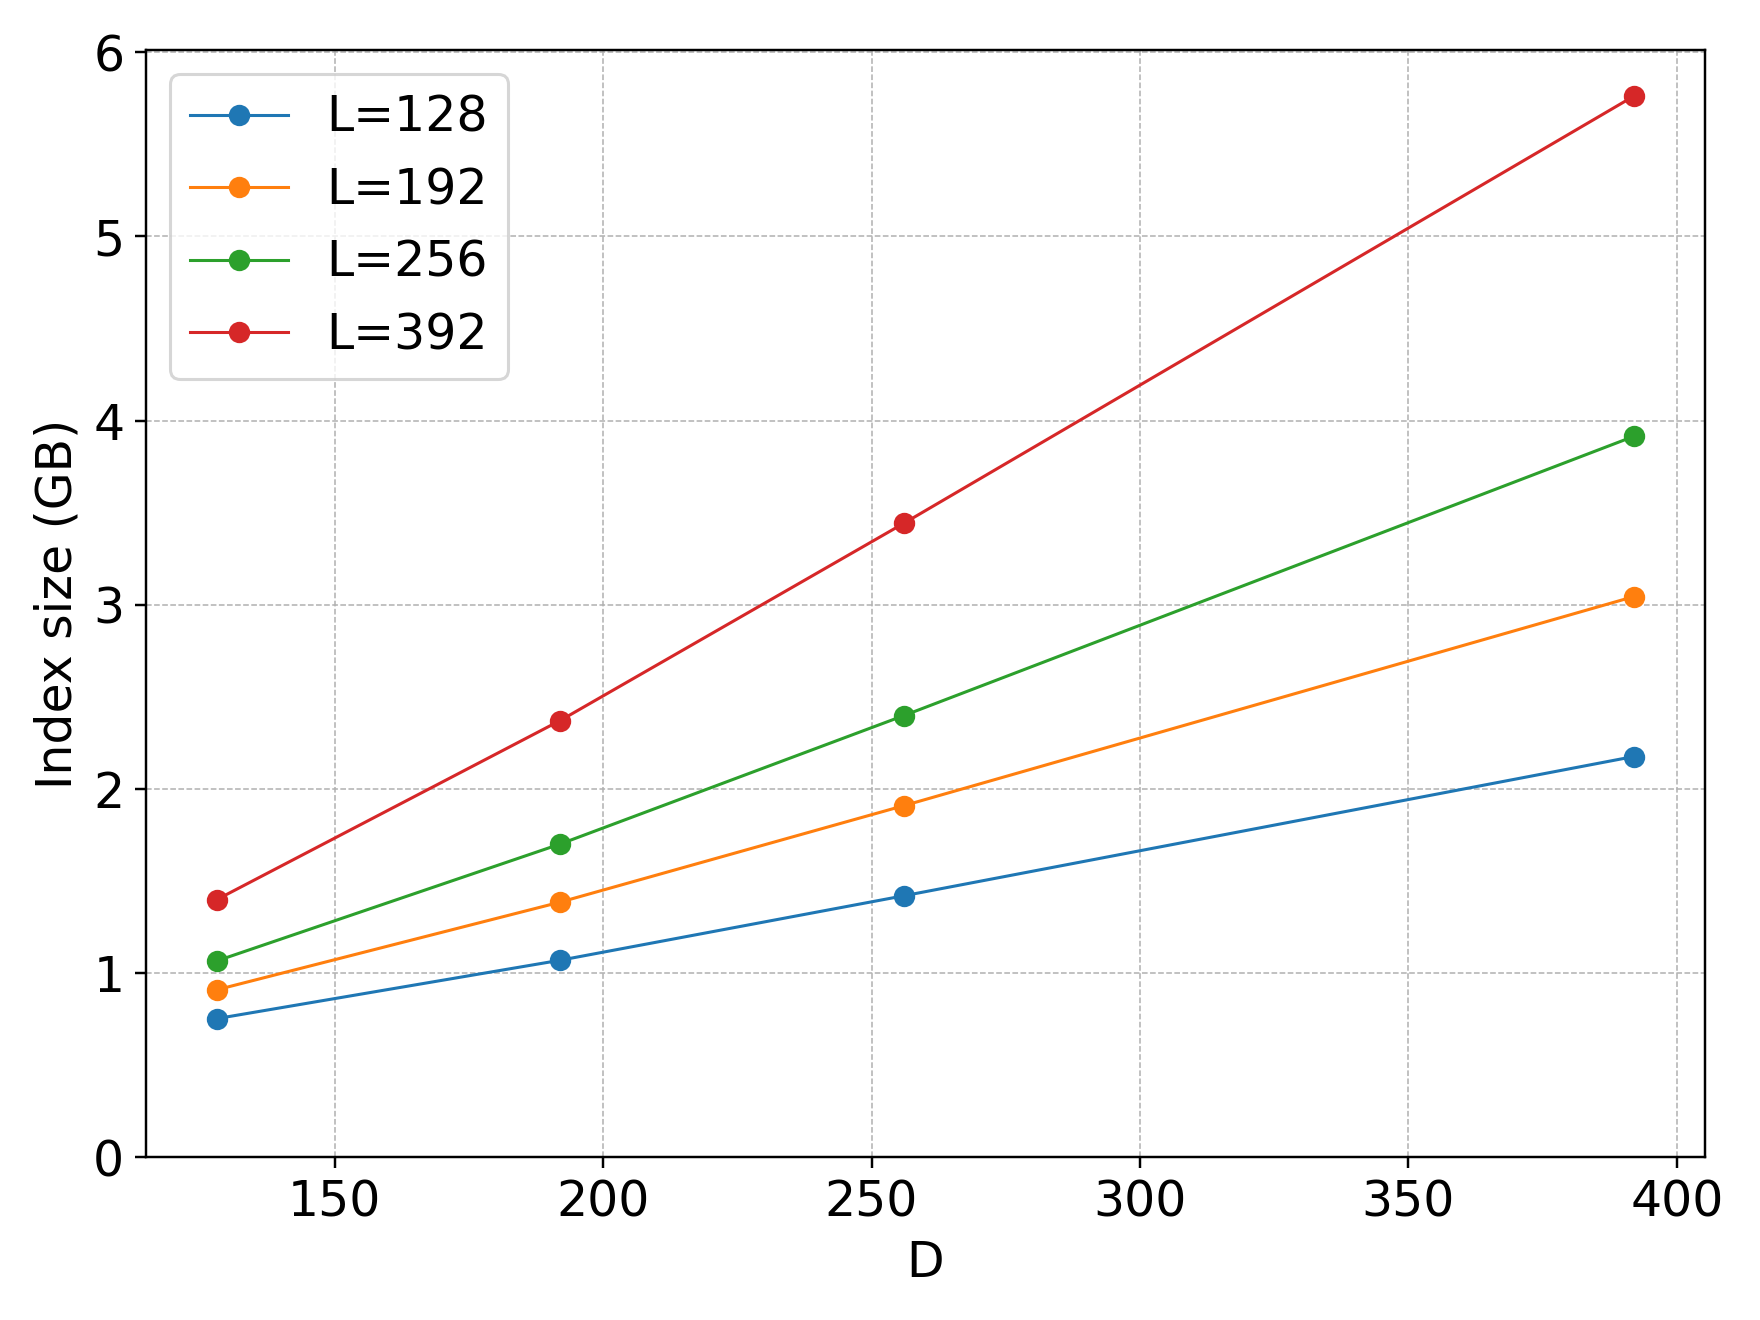
\includegraphics[width=\linewidth]{figs/plots/index-glv-ymlm/index_size_vs_D_lines_repeats_glove-100.png}
        \caption{\glv index size}
        \label{fig:glove-index-size}
    \end{subfigure}
    \hfill
    \begin{subfigure}{0.4\textwidth}
        \centering
        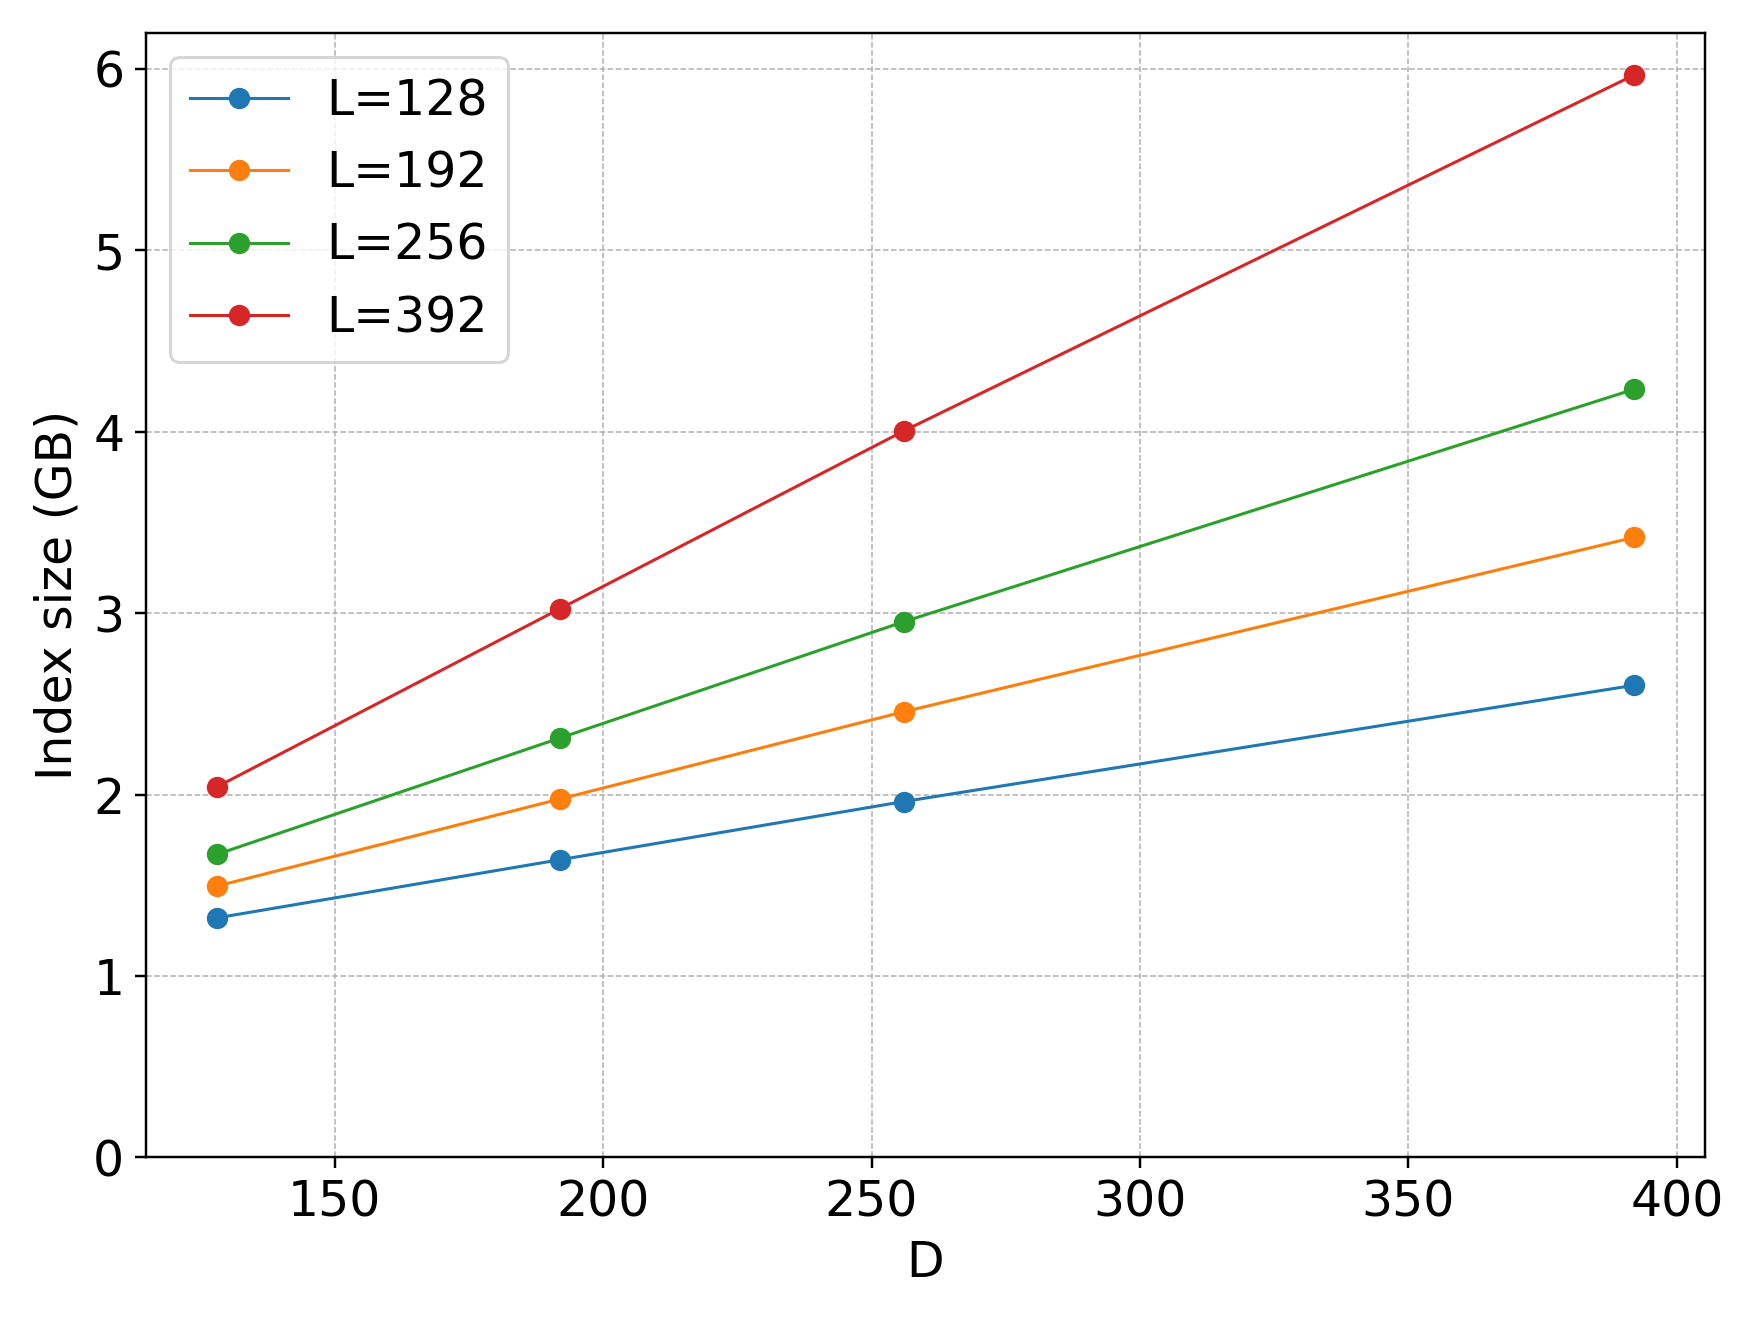
\includegraphics[width=\linewidth]{figs/plots/index-glv-ymlm/index_size_vs_D_lines_repeats_yahoo-minilm.png}
        \caption{\ymlm index size}
        \label{fig:yahoo-index-size}
    \end{subfigure}
    \hfill
    \begin{subfigure}{0.4\textwidth}
        \centering
        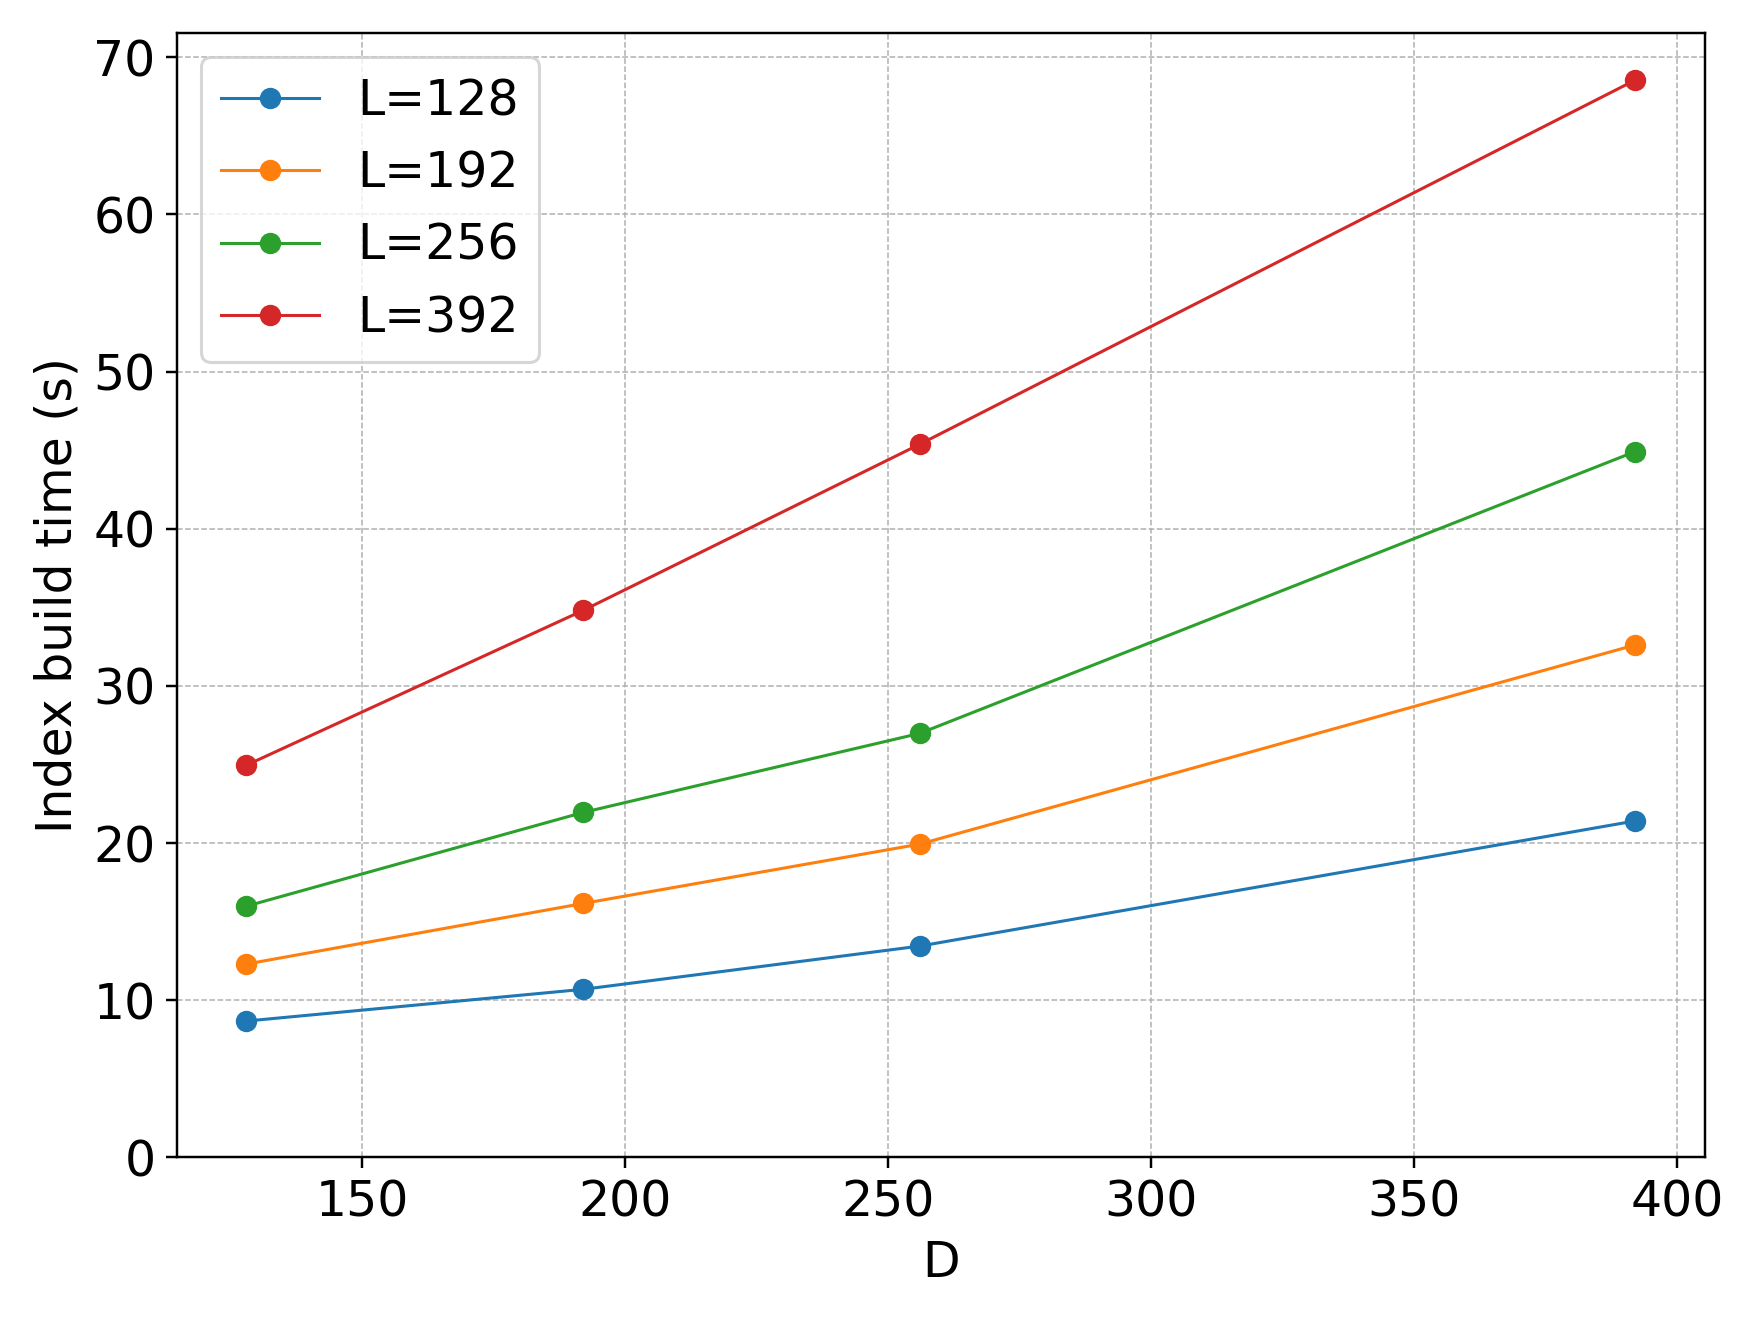
\includegraphics[width=\linewidth]{figs/plots/index-glv-ymlm/index_time_vs_D_lines_repeats_glove-100.png}
        \caption{\glv build time}
        \label{fig:glove-build-time}
    \end{subfigure}
    \hfill
    \begin{subfigure}{0.4\textwidth} 
        \centering
        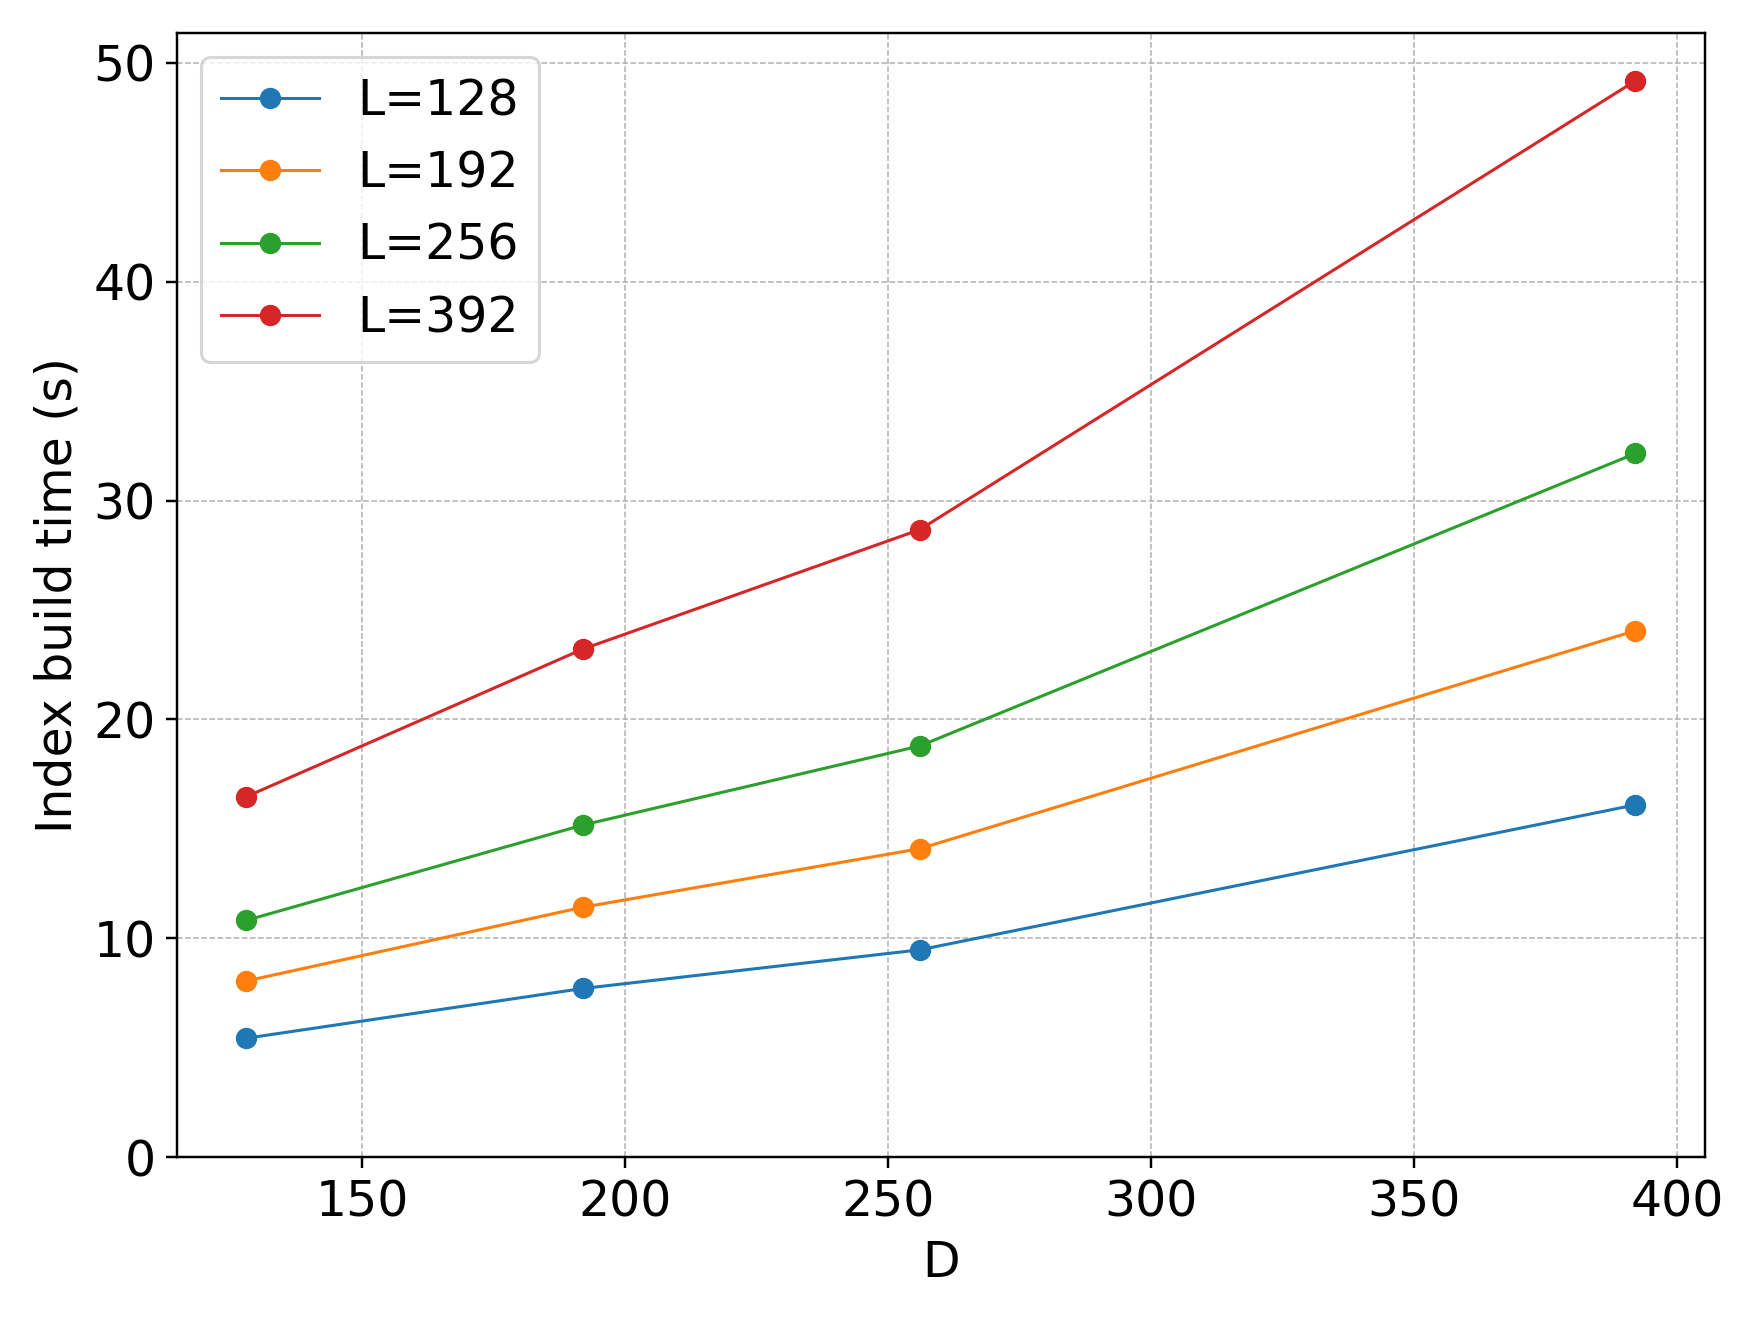
\includegraphics[width=\linewidth]{figs/plots/index-glv-ymlm/index_time_vs_D_lines_repeats_yahoo-minilm.png}
        \caption{\ymlm build time}
        \label{fig:yahoo-build-time}
    \end{subfigure}

    \caption{Indexing performance for varied $D$ and $L$ for \glv and \ymlm}
    \label{fig:index-perf-glove-yahoo}
\end{figure}

\alert{Perhaps add some comment on how we keep the value of D relatively low as compared to \fpp. Can say this is a practical consideration given the fact that large $D$ and $L$ create impractically large indices on the GPU}

\begin{table}[]
    \centering
    \begin{tabular}{c|c|c|c|c}
         Dataset & $L$ & $D$ & Build time (s) & Space (GB) \\
         \hline
        \gist & 16 & 16 &  $2.3$ & 3.58 \\ 
        \imgnt & 64 & 64 & $6.9$ & 1.35 \\ 
    \end{tabular}
    \caption{Indexing performance of \cf for GIST and ImageNet}
    \label{tab:gist-imagenet-indexing}
\end{table}

\begin{figure}[t]
    \centering
    \begin{subfigure}{0.45\textwidth}
        \centering
        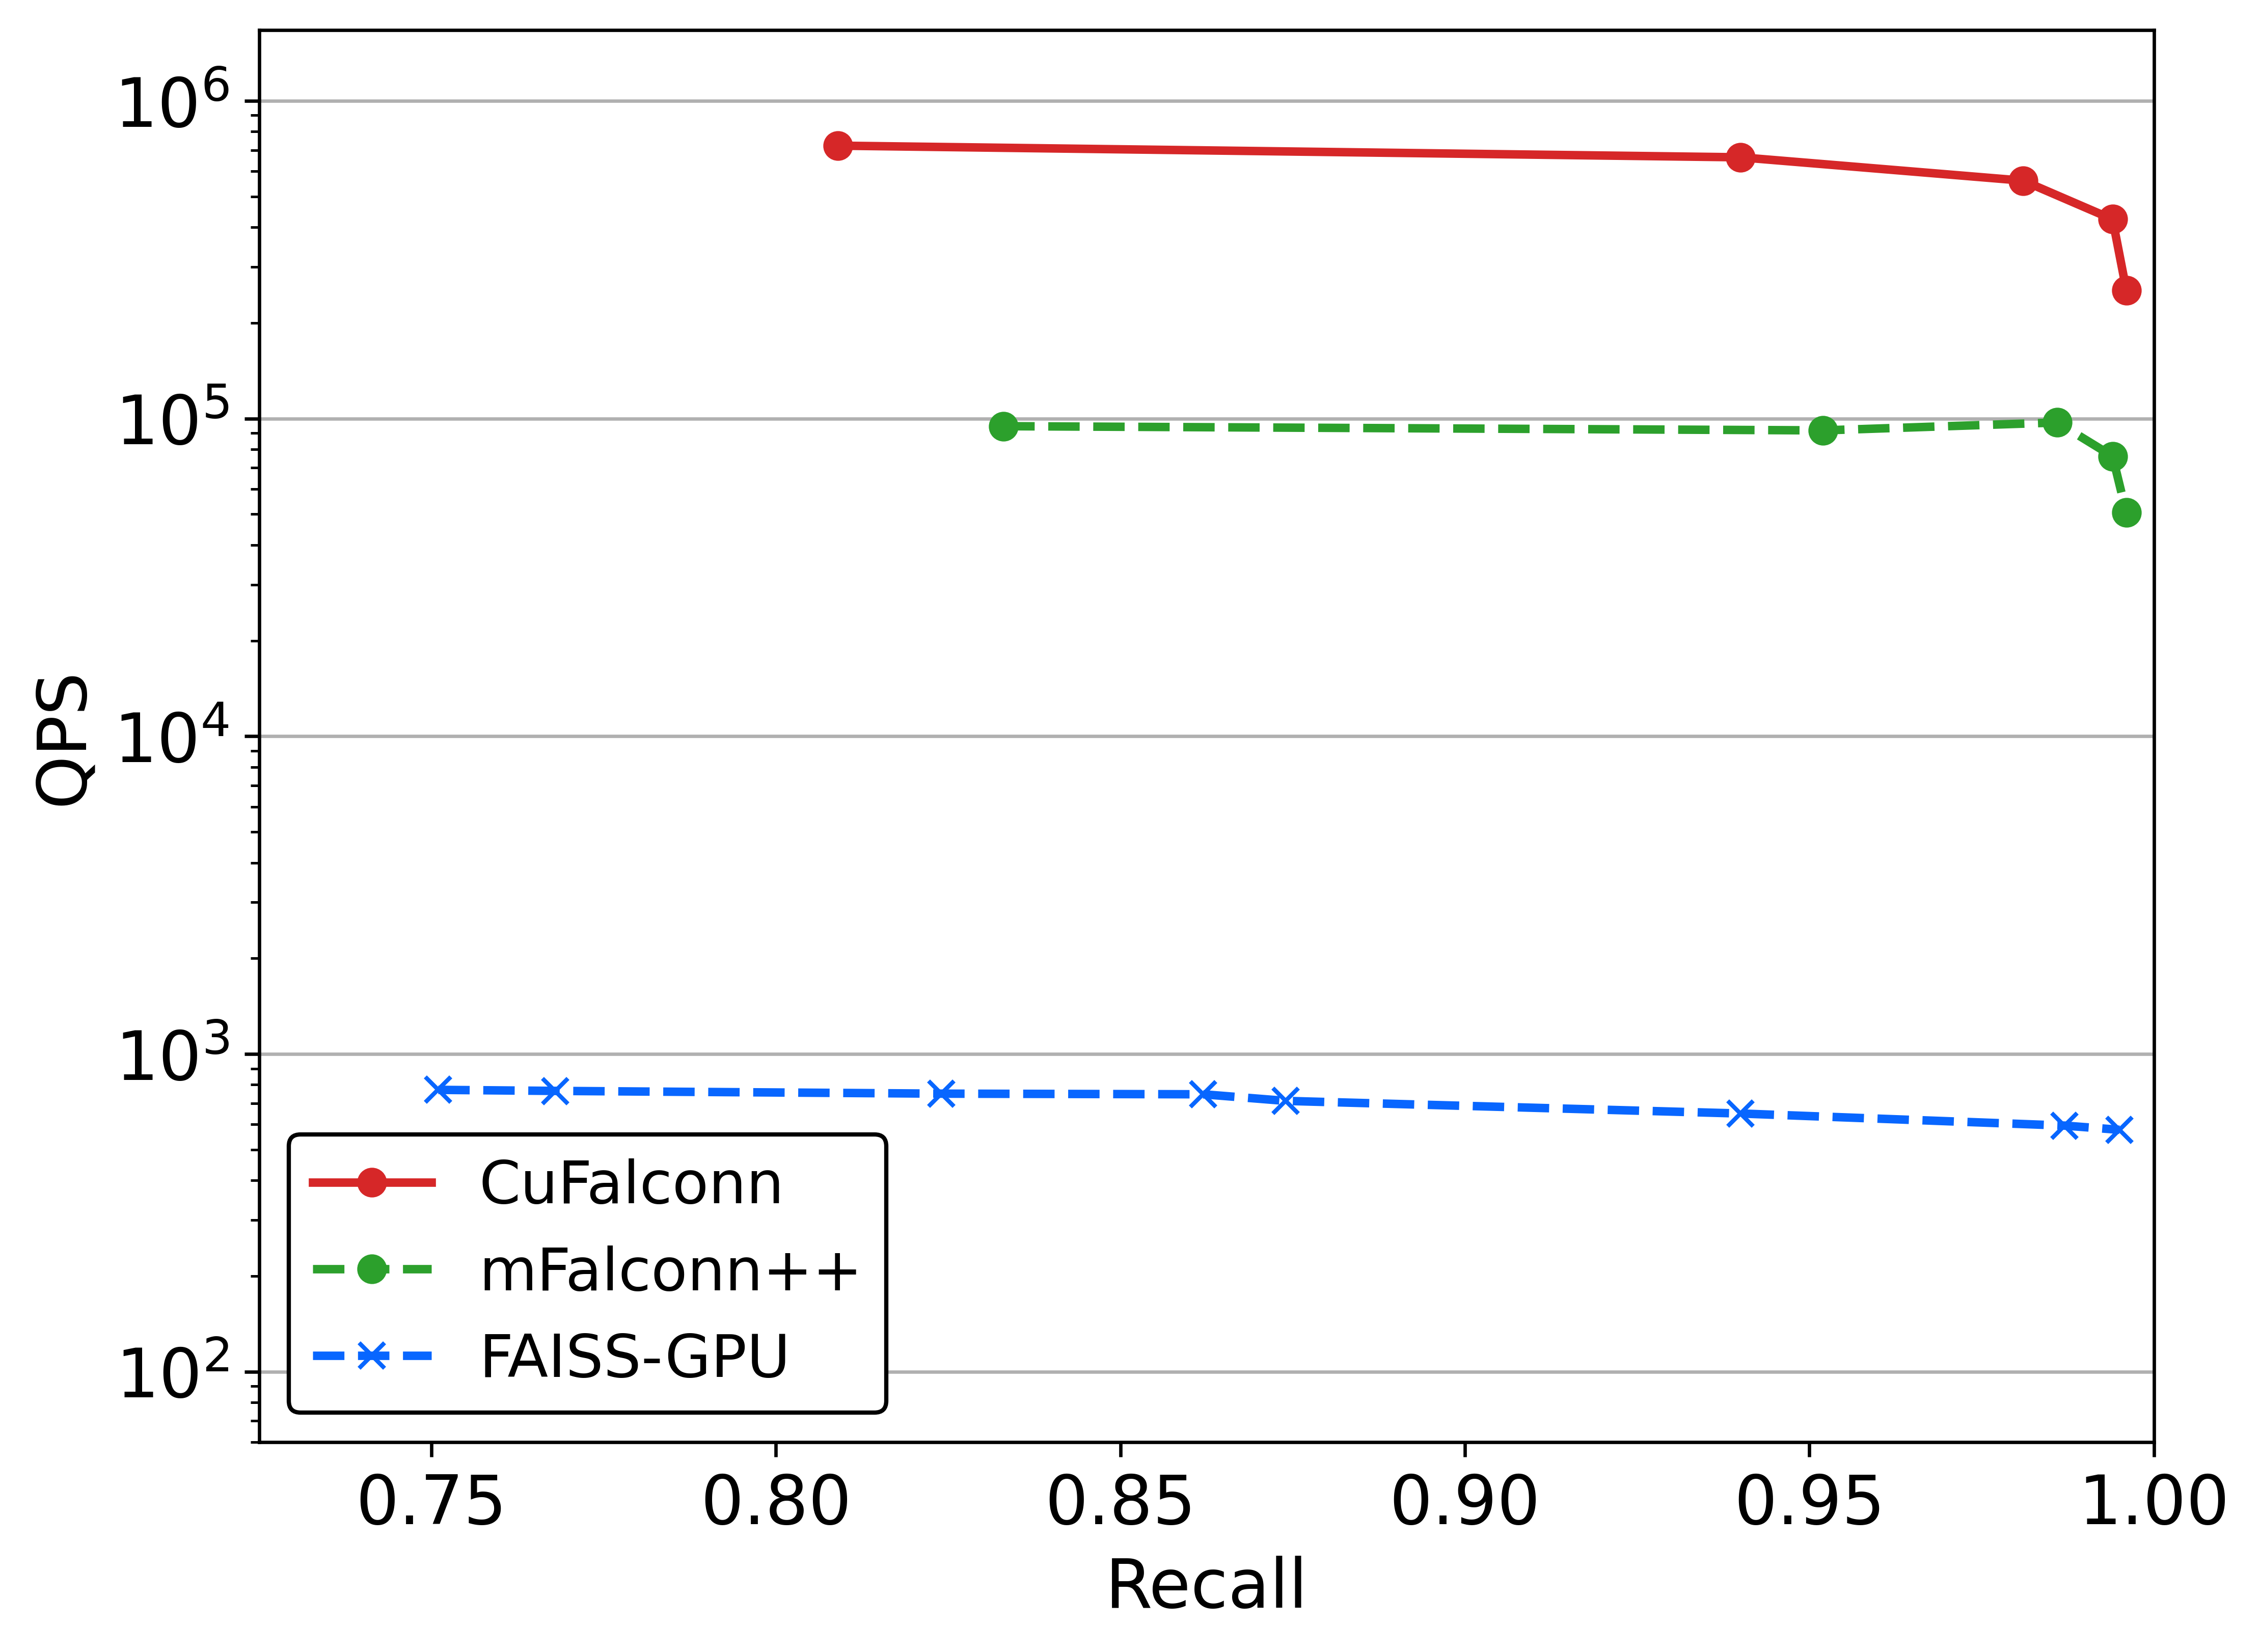
\includegraphics[width=\linewidth]{figs/plots/query-comparison/recall_qps_GIST_IP_faissp_ceosp.png}
        \caption{\gist IP}
        \label{fig:gist-query}
    \end{subfigure}
    \hfill
    \begin{subfigure}{0.45\textwidth}
        \centering
        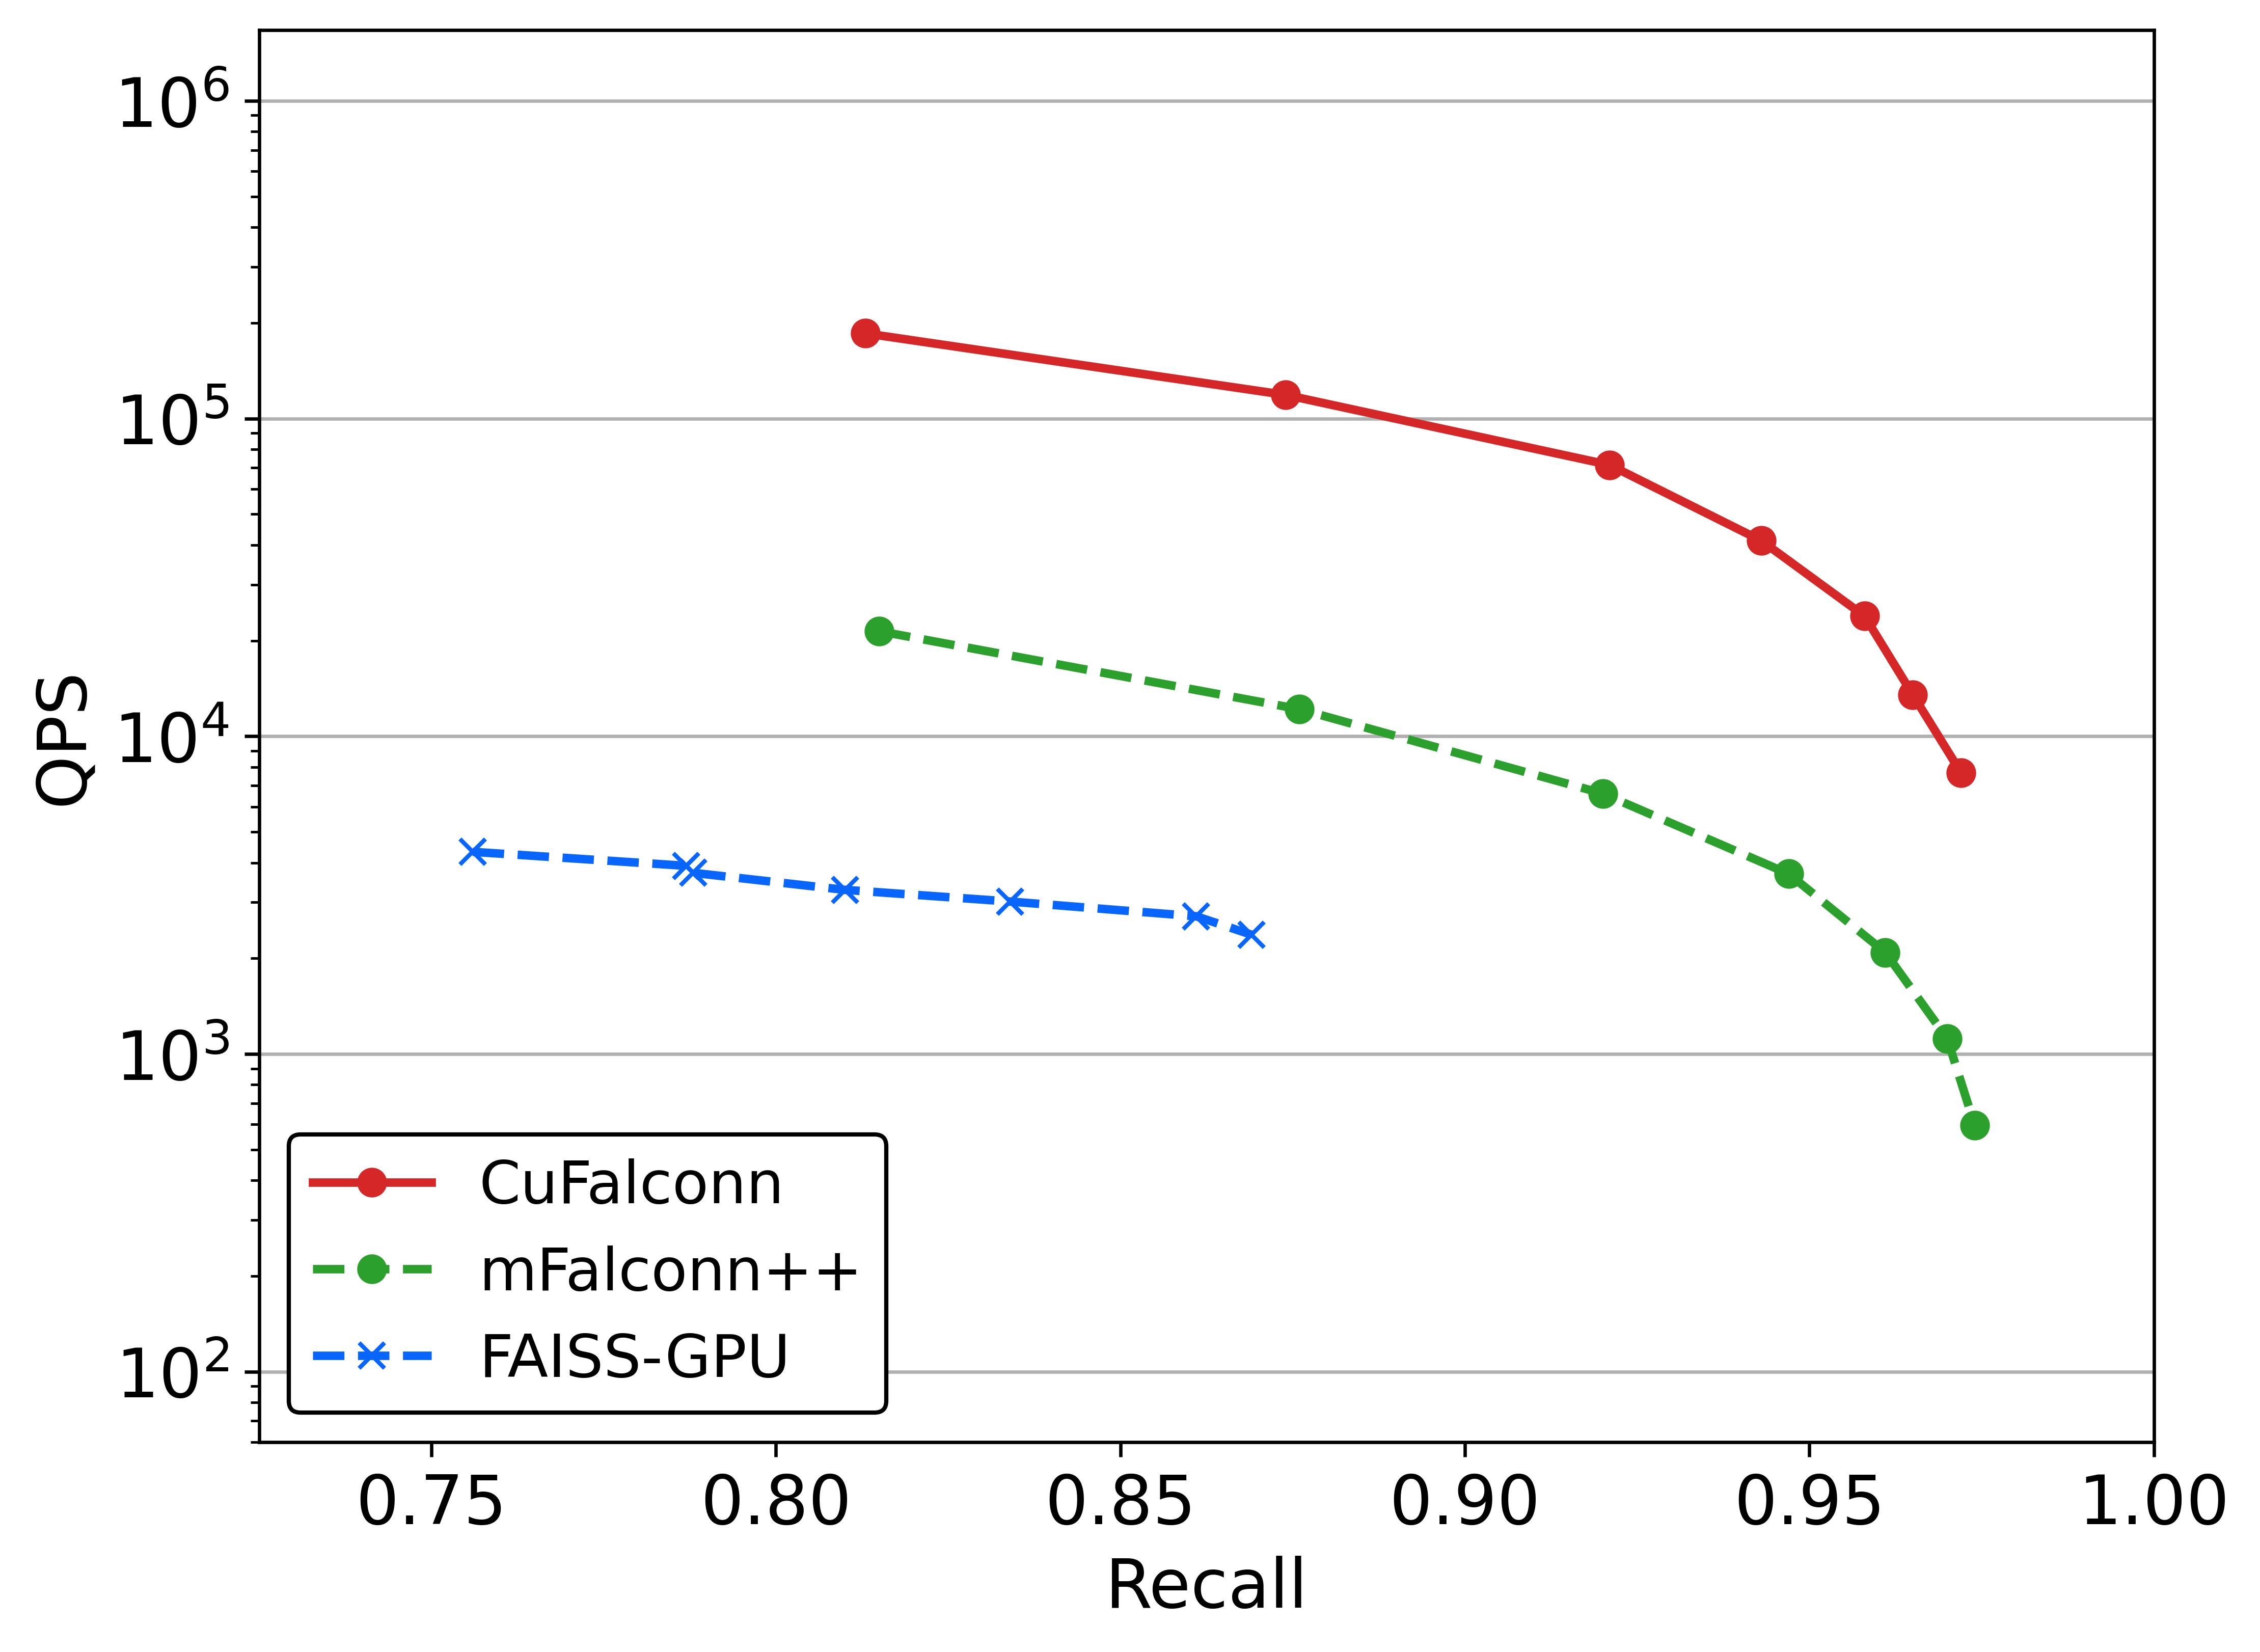
\includegraphics[width=\linewidth]{figs/plots/query-comparison/recall_qps_ImageNet_IP_faissp_ceosp.png}
        \caption{\imgnt IP}
        \label{fig:imagenet-query}
    \end{subfigure}
    
    \medskip

    \begin{subfigure}{0.45\textwidth}
        \centering
        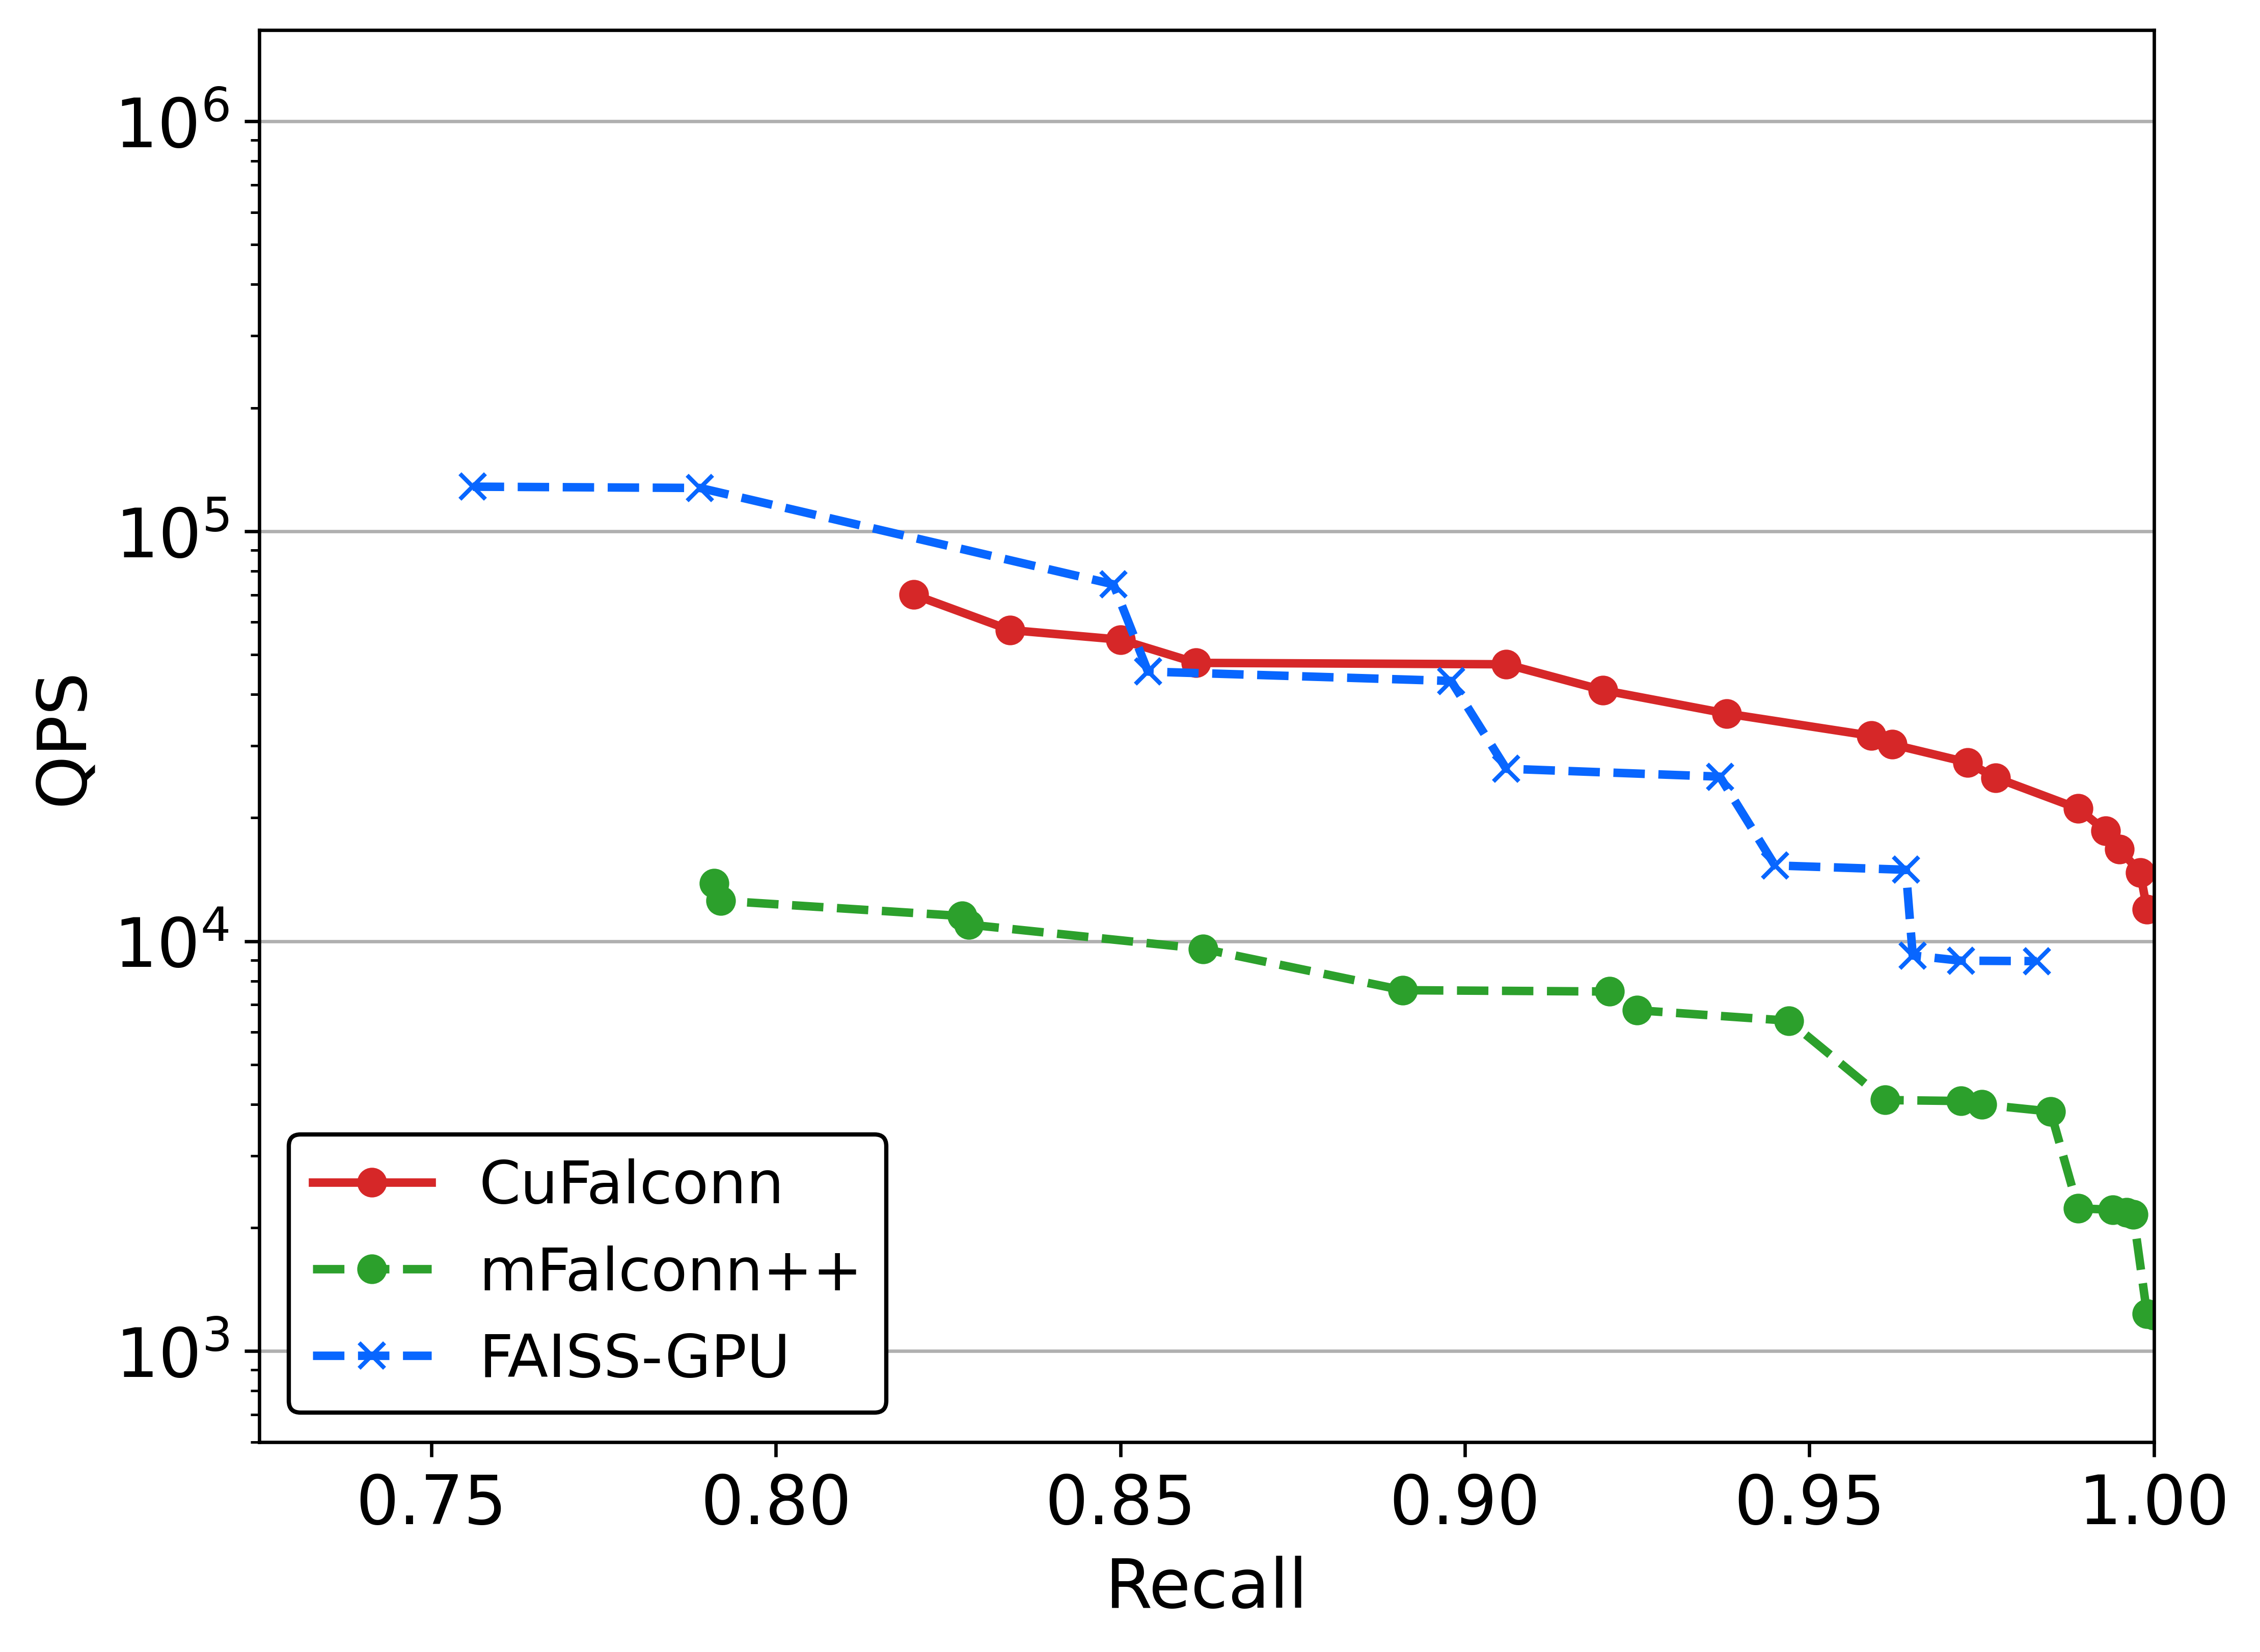
\includegraphics[width=\linewidth]{figs/plots/query-comparison/recall_qps_GloVe-100_COS_cufp_faissp_ceosp.png}
        \caption{\glv Angular}
        \label{fig:glove-query}
    \end{subfigure}
    \hfill
    \begin{subfigure}{0.45\textwidth} 
        \centering
        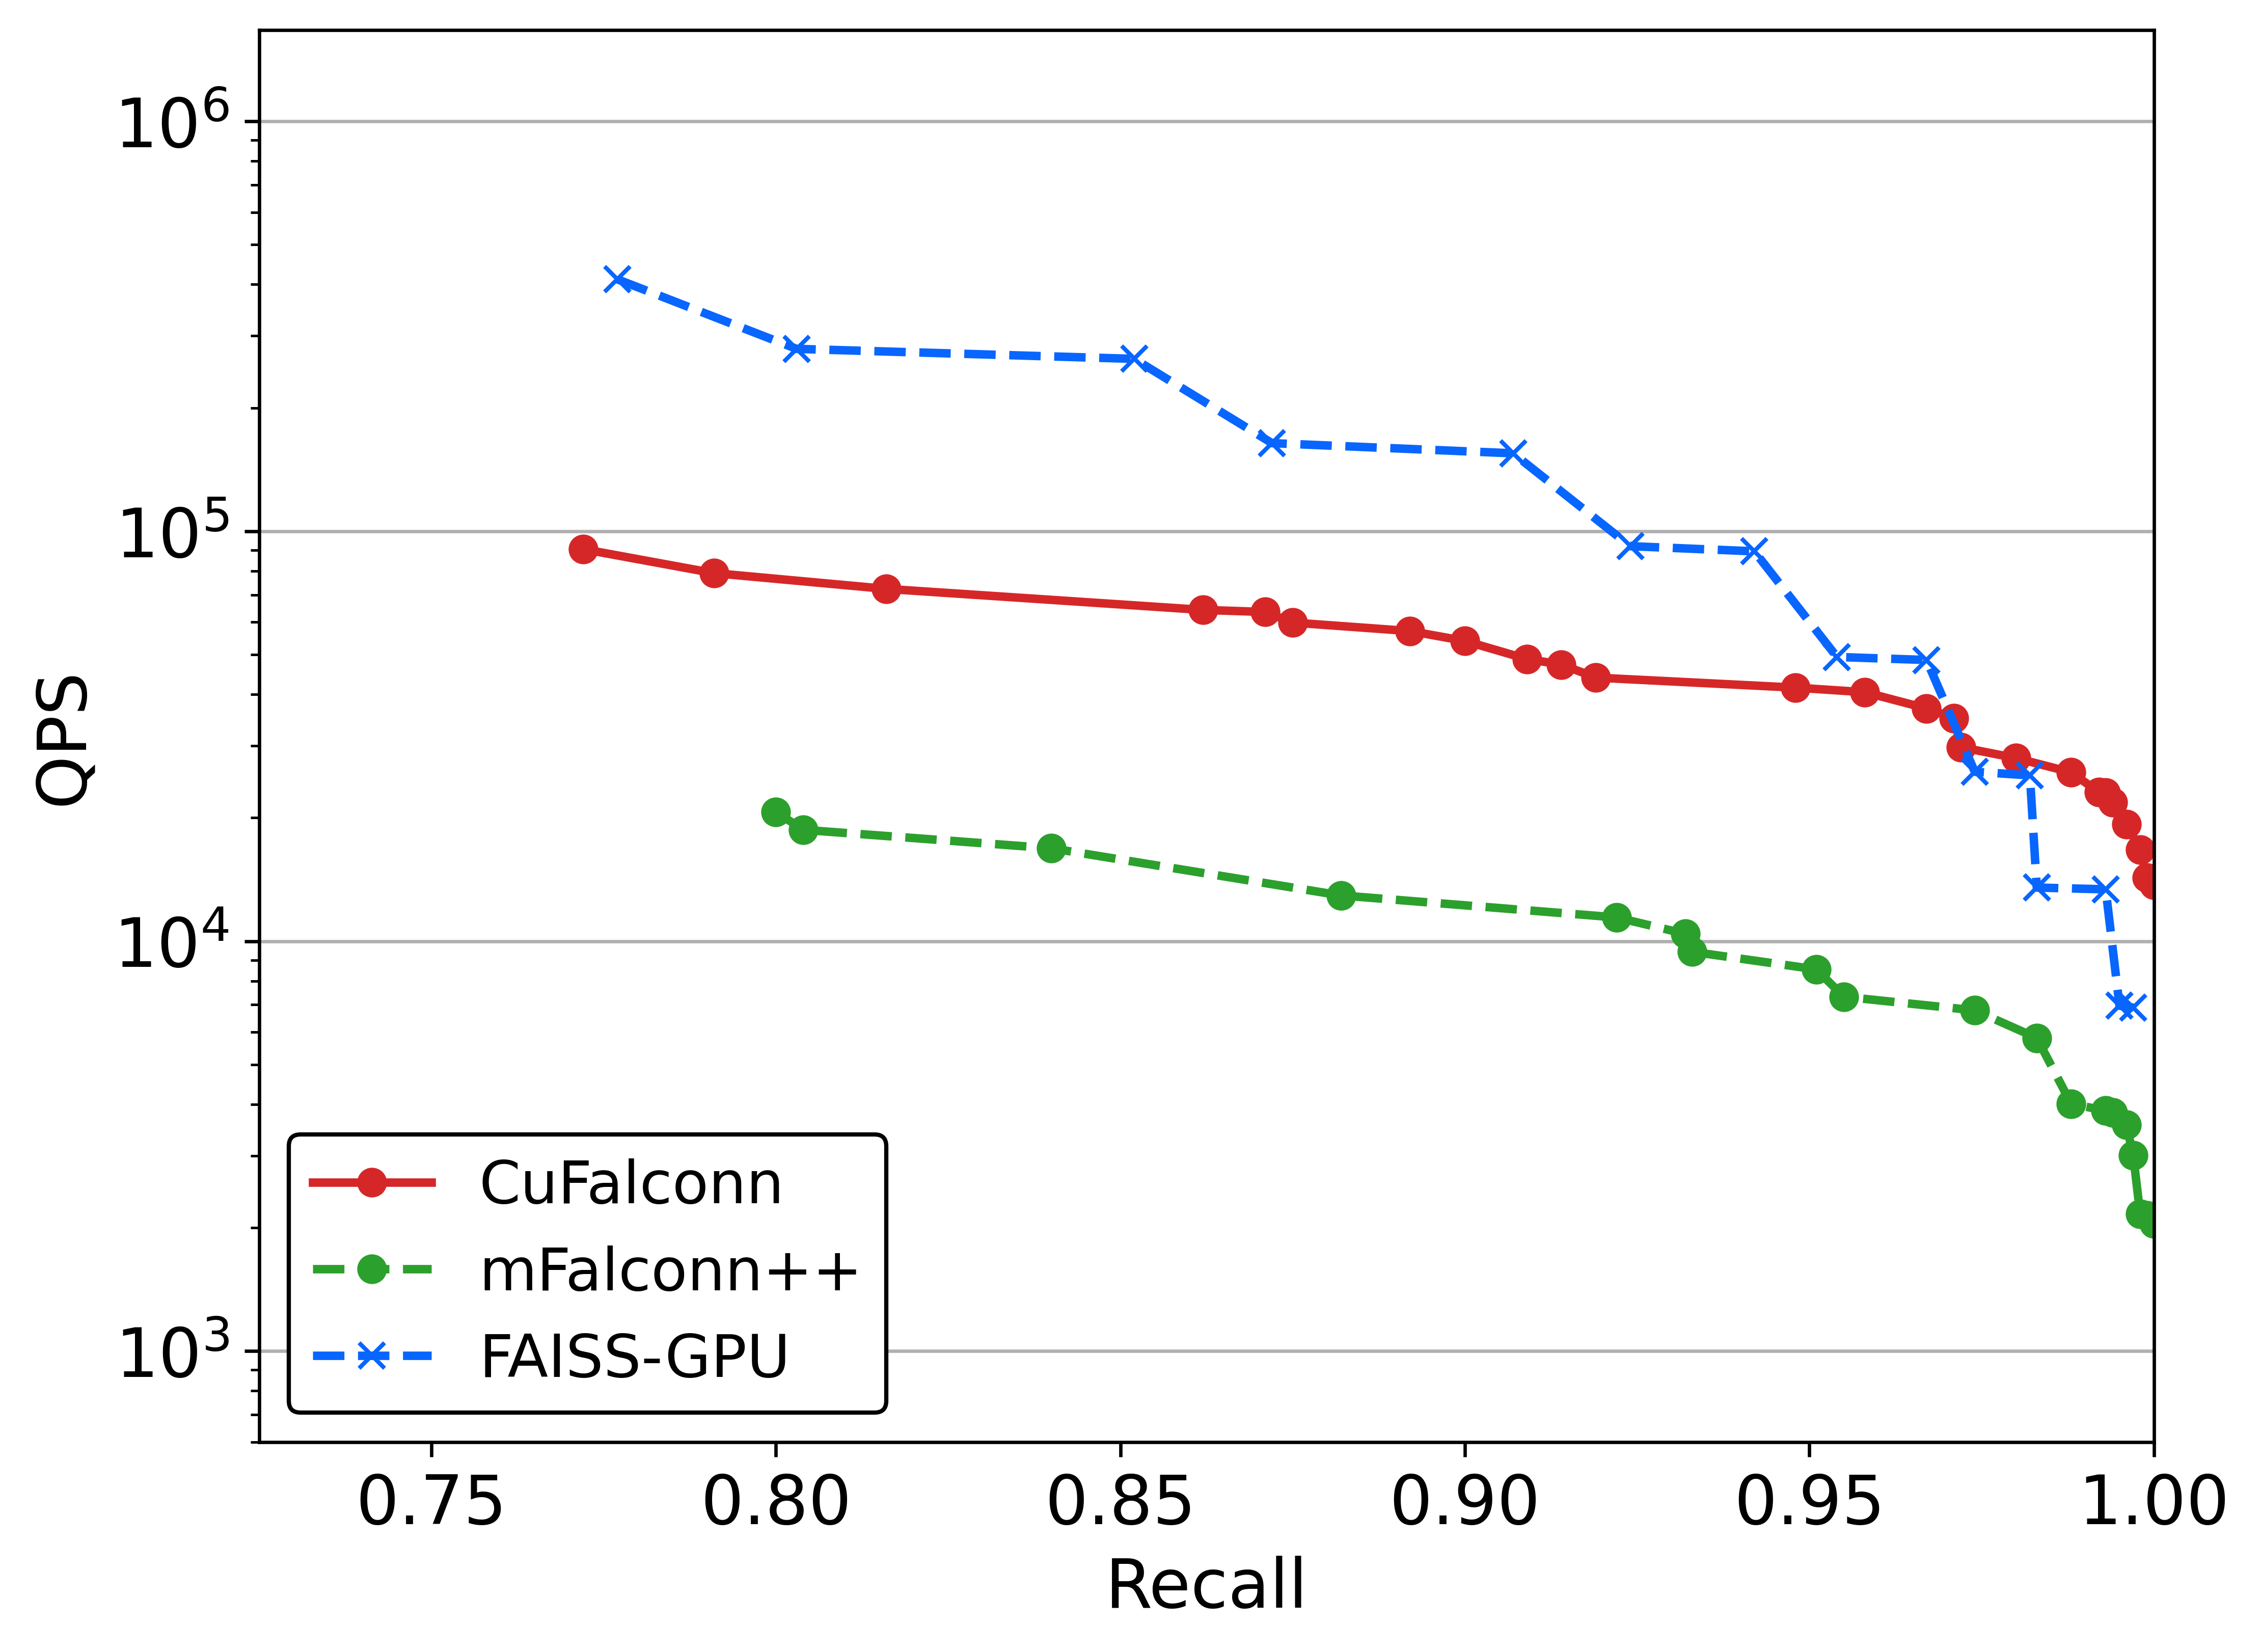
\includegraphics[width=\linewidth]{figs/plots/query-comparison/recall_qps_Yahoo-minilm_COS_cufp_faissp_ceosp.png}
        \caption{\ymlm Angular}
        \label{fig:yahoo-query}
    \end{subfigure}

    \caption{Querying performance on selected datasets}
    \label{fig:query-perf}
\end{figure}

\subsection{Comparison to \mfpp}
\label{sec:faiss-compare}

We compare the performance of \cf to \mfpp on all the datasets mentioned. Since they are equivalent algorithms, they can be run with identical parameters for both indexing and querying - allowing for a fair comparison. Consequently, we run \mfpp using the same parameters as \cf mentioned in Sec.~\ref{sec:dataset-perf}. 

\paragraph{Querying performance.} \cf has markedly faster querying faster querying than \mfpp. As shown by Fig.~\ref{fig:query-perf}, on high recall regimes \cf is generally approximately a magnitude faster on all datasets. Another noticeable pattern is that \cf and \mfpp recall-QPS curves have similar trajectories, indicating that \cf offers a stable and near query constant speed-up over \mfpp. 

\paragraph{Indexing performance.} \cf offers consistently faster index build times than \mfpp. For GIST and ImageNet, we found that the build times were approximately twice as fast - see Tab.~\ref{tab:cf-csh-gist-imagenet-index-speedup}. For a more detailed comparison though, we compared the build times across the various combinations of $D$ and $L$ in \ref{sec:dataset-perf} on \glv and \ymlm. Figure \ref{fig:cf-csh-index-speed}, shows the indexing build speed-up of \glv to \ymlm for a fixed $D$ and varied $L$. Interestingly, no single value of $D$ consistently yields the best indexing performance across the two datasets. On \glv, the relative ordering varies greatly, whereas on \ymlm, $D=128$ provides the highest indexing speed. However, this same configuration ($D=128$) is outperformed by other $D$ values on \glv. A general conclusion from the build-time speed-up analysis is that although \cf consistently outperforms \mfpp, the margin is smaller than might be anticipated. Given the substantially larger speed-ups observed during querying (Fig.~\ref{fig:query-perf}), one might expect indexing to exhibit comparable acceleration. Instead, the indexing improvements are noticeably more modest. Future work could therefore investigate further accelerating the indexing stage, potentially through a fully GPU-resident approach. We do not compare the indexing space of \mfpp to \cf, as they are practically identical in this respect since they implement the same underlying algorithm.

\begin{table}[]
    \centering
    \begin{tabular}{c| lcc}
         Dataset & \cf & \mfpp & Speedup \\ 
         \hline
        GIST &  $2.3$s & $6.0$s &  $2.6 \times$ \\ 
        ImageNet & $6.9$s & $11.2$s & $1.6 \times $\\ 
    \end{tabular}   
    \caption{Comparing indexing build times of \cf to \mfpp.}
    \label{tab:cf-csh-gist-imagenet-index-speedup}
\end{table}

\begin{figure}
    \centering
    \begin{subfigure}{0.45\textwidth}
        \label{fig:glove-index}
        \centering
        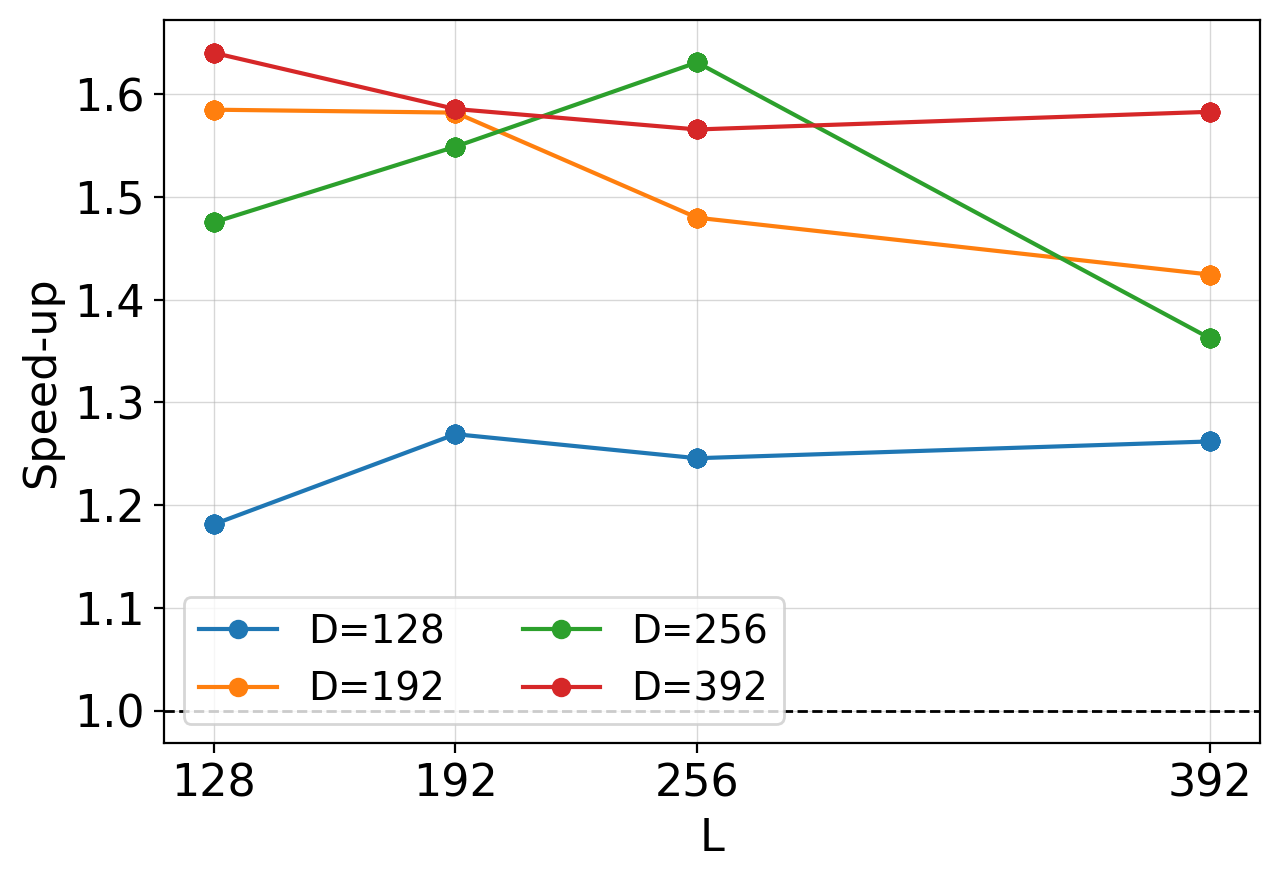
\includegraphics[width=\linewidth]{figs/plots/index-speedup/index_speedup_glove-100_COS.png}
        \caption{\glv}
    \end{subfigure}
    \hfill
    \begin{subfigure}{0.45\textwidth}
        \label{fig:yahoo-index}
        \centering
        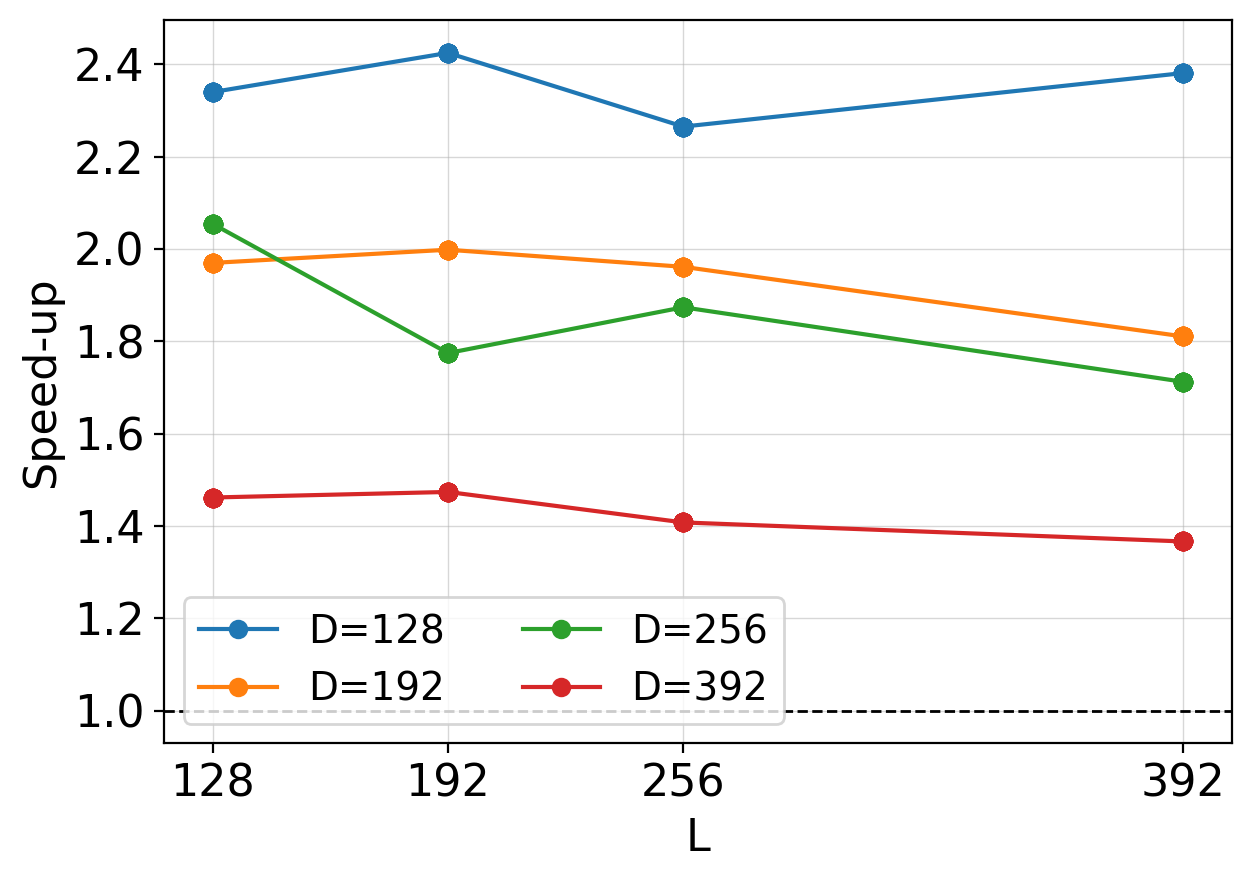
\includegraphics[width=\linewidth]{figs/plots/index-speedup/index_speedup_yahoo-minilm_COS.png}
        \caption{\ymlm}
    \end{subfigure}

    \caption{Comparing the indexing time speed-up of \cf to \mfpp for different combinations of $D$ and $L$}
    \label{fig:cf-csh-index-speed}
\end{figure}

\subsection{Comparison to \fgpu}

We evaluate FAISS-GPU over powers-of-two sweeps of $nList \in [256, 8192]$ and $nProbe \in [1, 1024]$. Larger $nList$ values produce finer partitions, permitting proportionally larger $nProbe$ settings and thus larger candidate sets per query. This follows the protocol followed by ANN Benchmarks to evaluate FAISS-IVF algorithms ~\cite{aumuller2020ann}. Table~\ref{tab:faiss-params} lists all configurations run, note that results are only reported for configurations achieving high recall.

\begin{table}[h]
    \centering
    \begin{tabular}{c | l}
    $nList$ & $nProbe$ \\
    \hline
    256  & 1, 2, 4, 8, 16, 32 \\
    512  & 1, 2, 4, 8, 16, 32, 64 \\
    1024 & 1, 2, 4, 8, 16, 32, 64, 128 \\
    2048 & 1, 2, 4, 8, 16, 32, 64, 128, 256 \\
    4096 & 1, 2, 4, 8, 16, 32, 64, 128, 256, 512 \\
    8192 & 1, 2, 4, 8, 16, 32, 64, 128, 256, 512, 1024 \\
    \end{tabular}
    \caption{FAISS-GPU $nList$ and $nProbe$ settings}
    \label{tab:faiss-params}
\end{table}

We plot the Pareto Frontier of querying results for \fgpu on all 4 datasets in Fig.~\ref{fig:query-perf} Using these results, we can see that the performance contrast between \cf and FAISS-GPU varies across datasets. For GIST and ImageNet, \cf generally outperforms FAISS-GPU - with a striking several orders of magnitude speed up on GIST. On ImageNet, FAISS-GPU struggles to attain a recall above $0.85$, despite attain results well above this threshold for the other datasets using identical indexing and querying parameters. On \glv and \ymlm, the performance between \cf and \fgpu is more competitive. On \glv, \cf beats \fgpu for recalls larger than $\approx 0.9$, a similar effect exists for \ymlm but for recalls above $\approx 0.975$.

Another noticeable phenomenon is that generally \cf has more stable performance than \fgpu particularly on \glv and \ymlm. The range of QPS values for \fpp on these datasets differs by more than a magnitude, while for \cf, these are within $10^5$ and $10^4$. We thus conclude that \cf can offer more consistent speed and accuracy trade-offs for some datasets. 

\alert{Should we be mentioning more here on indexing metrics - build time and space for faiss?}

\subsection{Ablation Study of $m$ on \glv}
\label{sec:ablation-glove}

We perform an ablation experiment using GloVe-100 on the role of the max bucket size $m$ on high recall regimes. For this experiment we set $L = D = 128$, $iProbes = 2$, as this had the fastest build time (for $m$ = 8) out of all configurations investigated for GloVe-100. We vary $m$ from the set $\{8, 16, 32, 64, 128\}$. For each $m$, we choose $qProbes$ over powers of two in the range $[8, 16384]$, and include intermediate half-step values to extend up to $24576$. More formally, we take $qProbes$ from the set $V_{qP}$ shown in Eq.~\ref{eq:set-V}. We then restrict attention to results attaining a recall of at-least $0.75$.

\begin{equation}
    V_{qP} = \{\, 2^i \mid i = 3,\dots,14 \,\}
    \;\cup\;
    \left\{\, 3 \cdot 2^{i-1} \mid i = 3,\dots,14 \,\right\}.
    \label{eq:set-V}
\end{equation}

Not surprisingly, as shown by Fig.~\ref{fig:index-size-ablation-m}, the size of an index generally increases as $m$ increases - in expectation, buckets contain more points. Another effect is that index build time is proportional to $m$, shown in Fig.~\ref{fig:index-time-ablation-m}. This is likely due to the non-trivial round trip data transfer costs between and CPU and GPU being magnified by a larger index - more data needs to be transferred between the two processors.

As show in Fig.~\ref{fig:recall-qps-ablation-m} larger buckets can generally increase the speed of queries. This is primarily due to the fact that larger buckets require \emph{less} candidates per query to achieve a high recall. This effect is illustrated in Fig.~\ref{fig:recall-candidates-ablation-m}, on average, queries need less candidates from larger buckets to achieve higher recall. For example for a recall $\approx 0.925$, $m = 8$ and $m=128$ can achieve this with approximately $97K$ and $27K$ candidates respectively - an almost $4$ fold difference. This effect is presumably caused by smaller buckets pruning out good candidates for a given query. Due to the probabilistic nature of LSH, the top points in the closest buckets to a query are only probabilistically close to a query. Consequently, when bucket truncation from a low $m$ can discard true nearest neighbours to a query because of their low score priority in a bucket. We can conclude that increasing $m$ generally can improve the accuracy-speed trade-off of CuFalconn. However, this advantage comes at clear cost of longer build times and larger index size. 

\alert{Perhaps a more detailed analysis of relationship - is there some non-linearity that could be at play - the relationship could be more detailed than simple proportionality. Maybe this conclusion lacks nuance.}

\begin{figure}[t]
    \begin{subfigure}{0.45\textwidth}
        \centering
        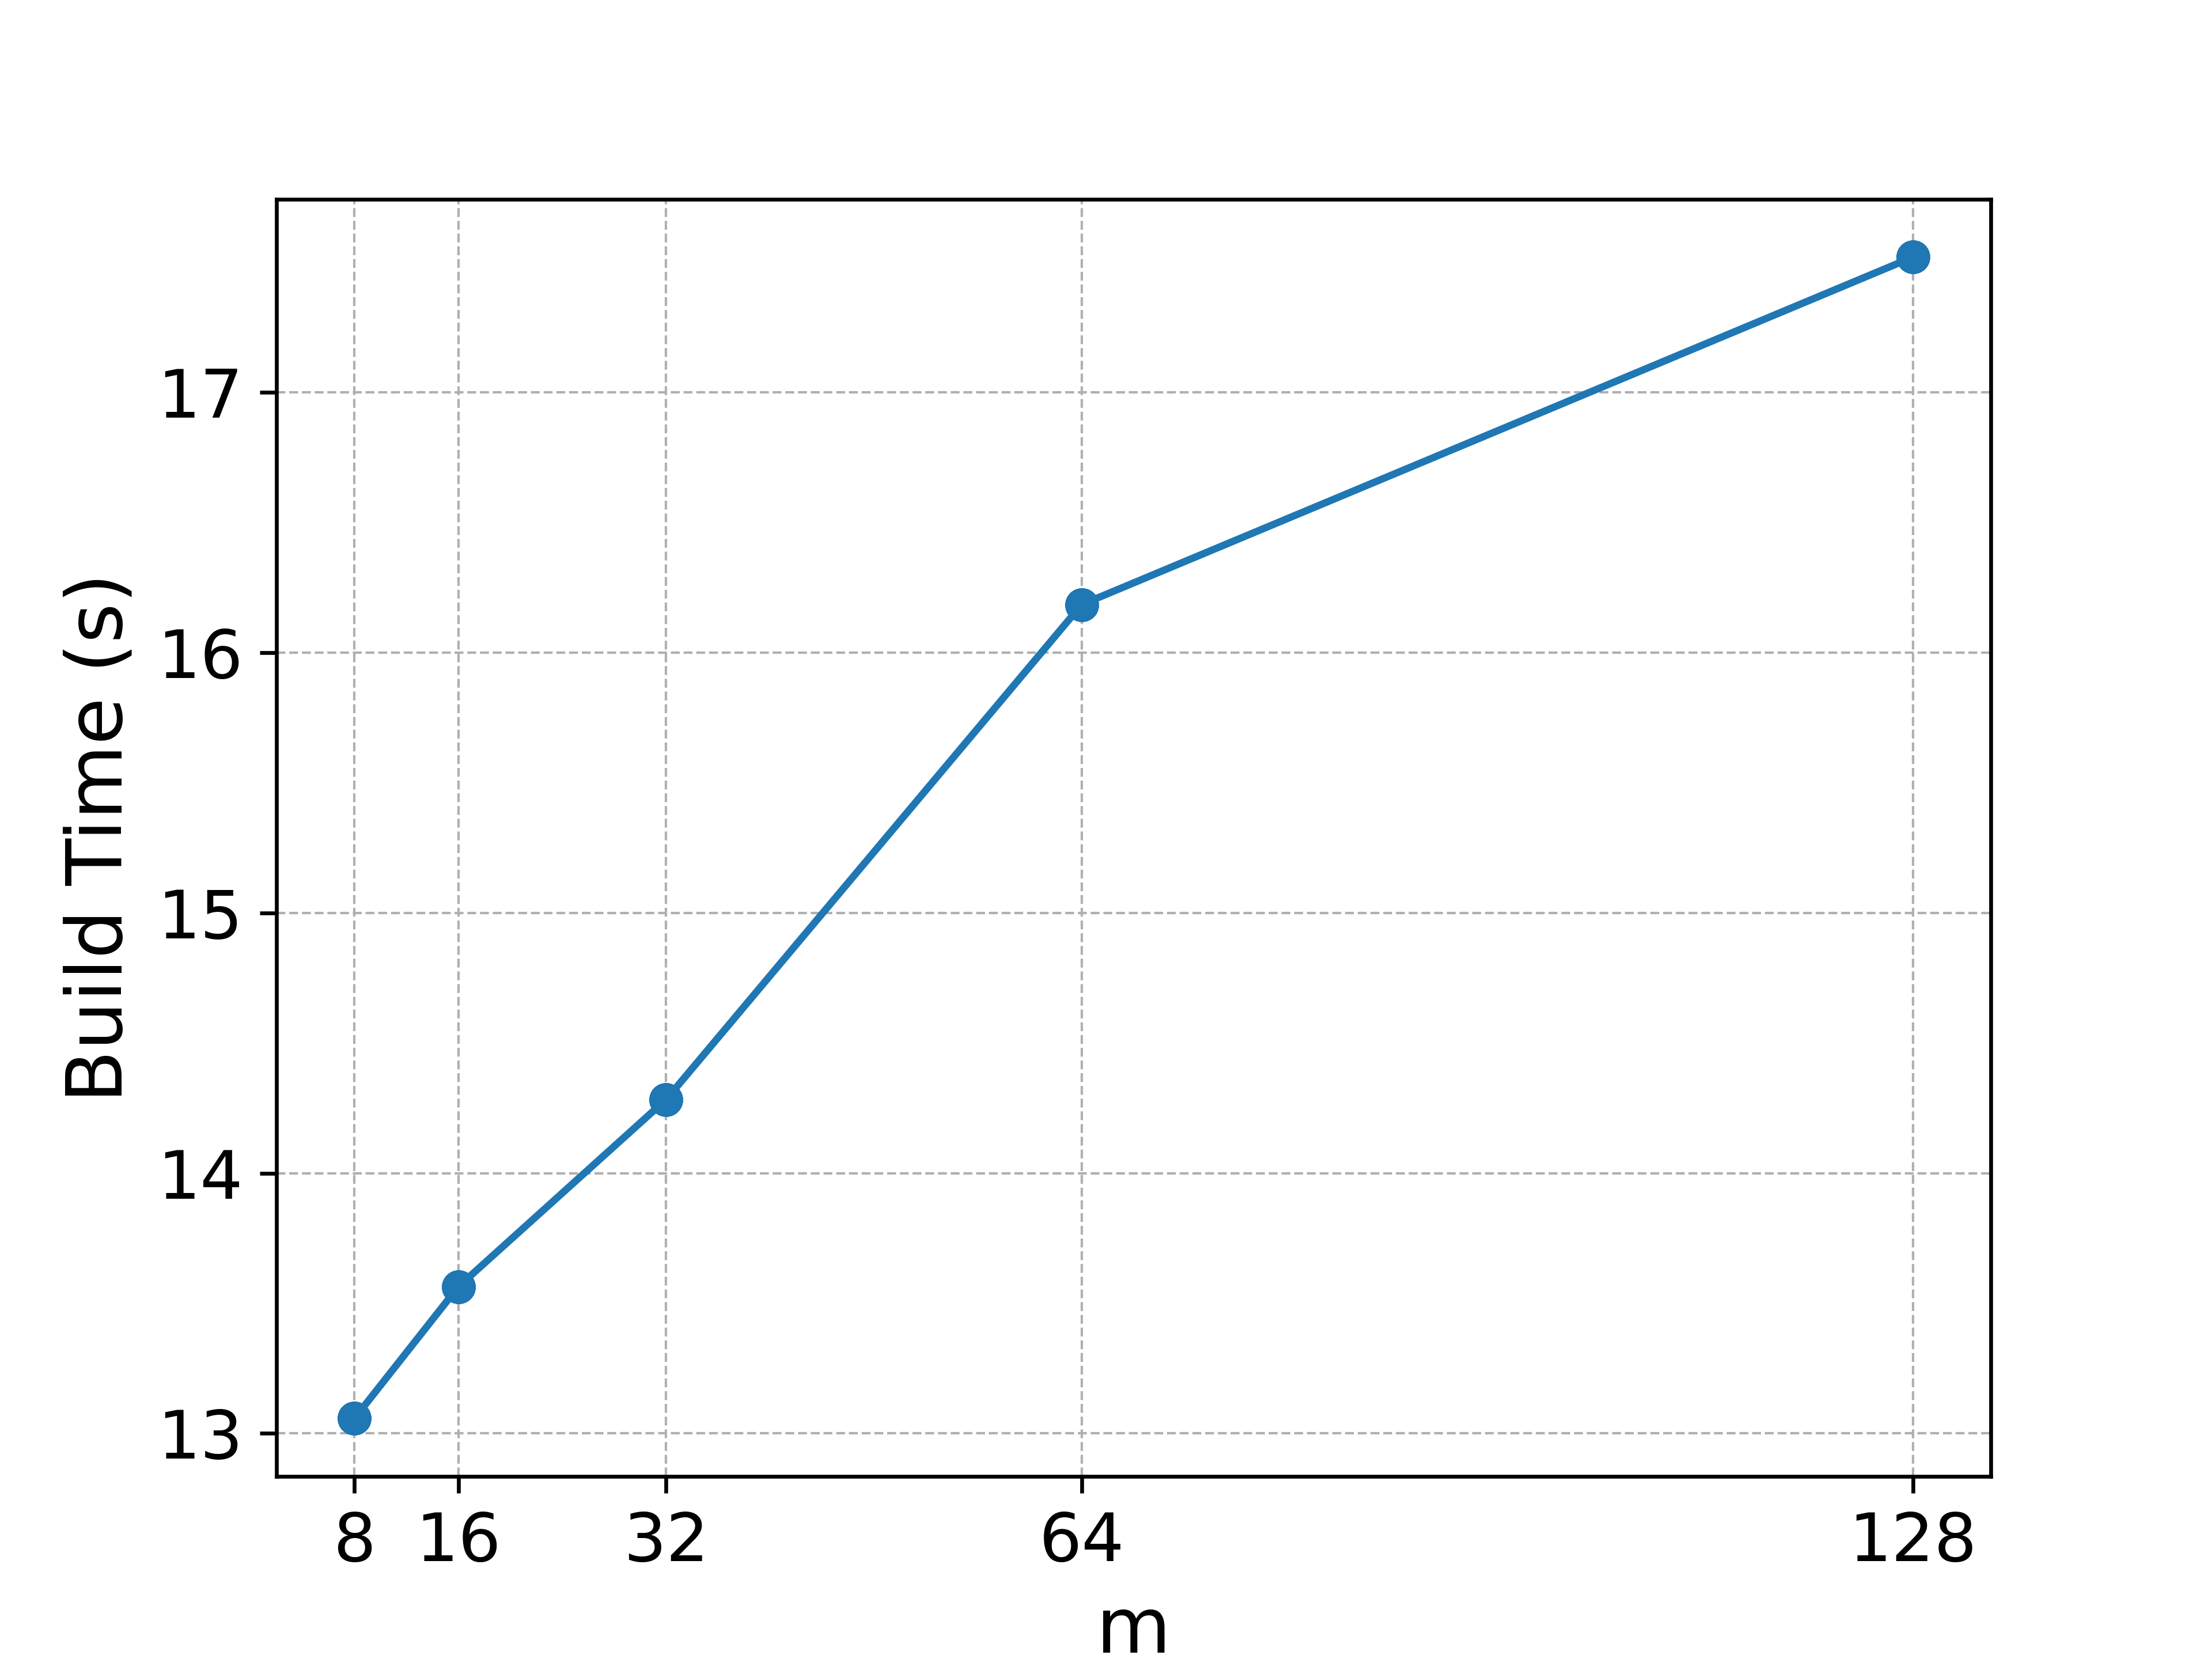
\includegraphics[width=\linewidth]{figs/plots/ablation-m/index_build_time_vs_m_glove-100.png}
        \caption{Index build time vs $m$}
        \label{fig:index-time-ablation-m}
    \end{subfigure}
    \hfill
    \begin{subfigure}{0.45\textwidth}
        \centering
        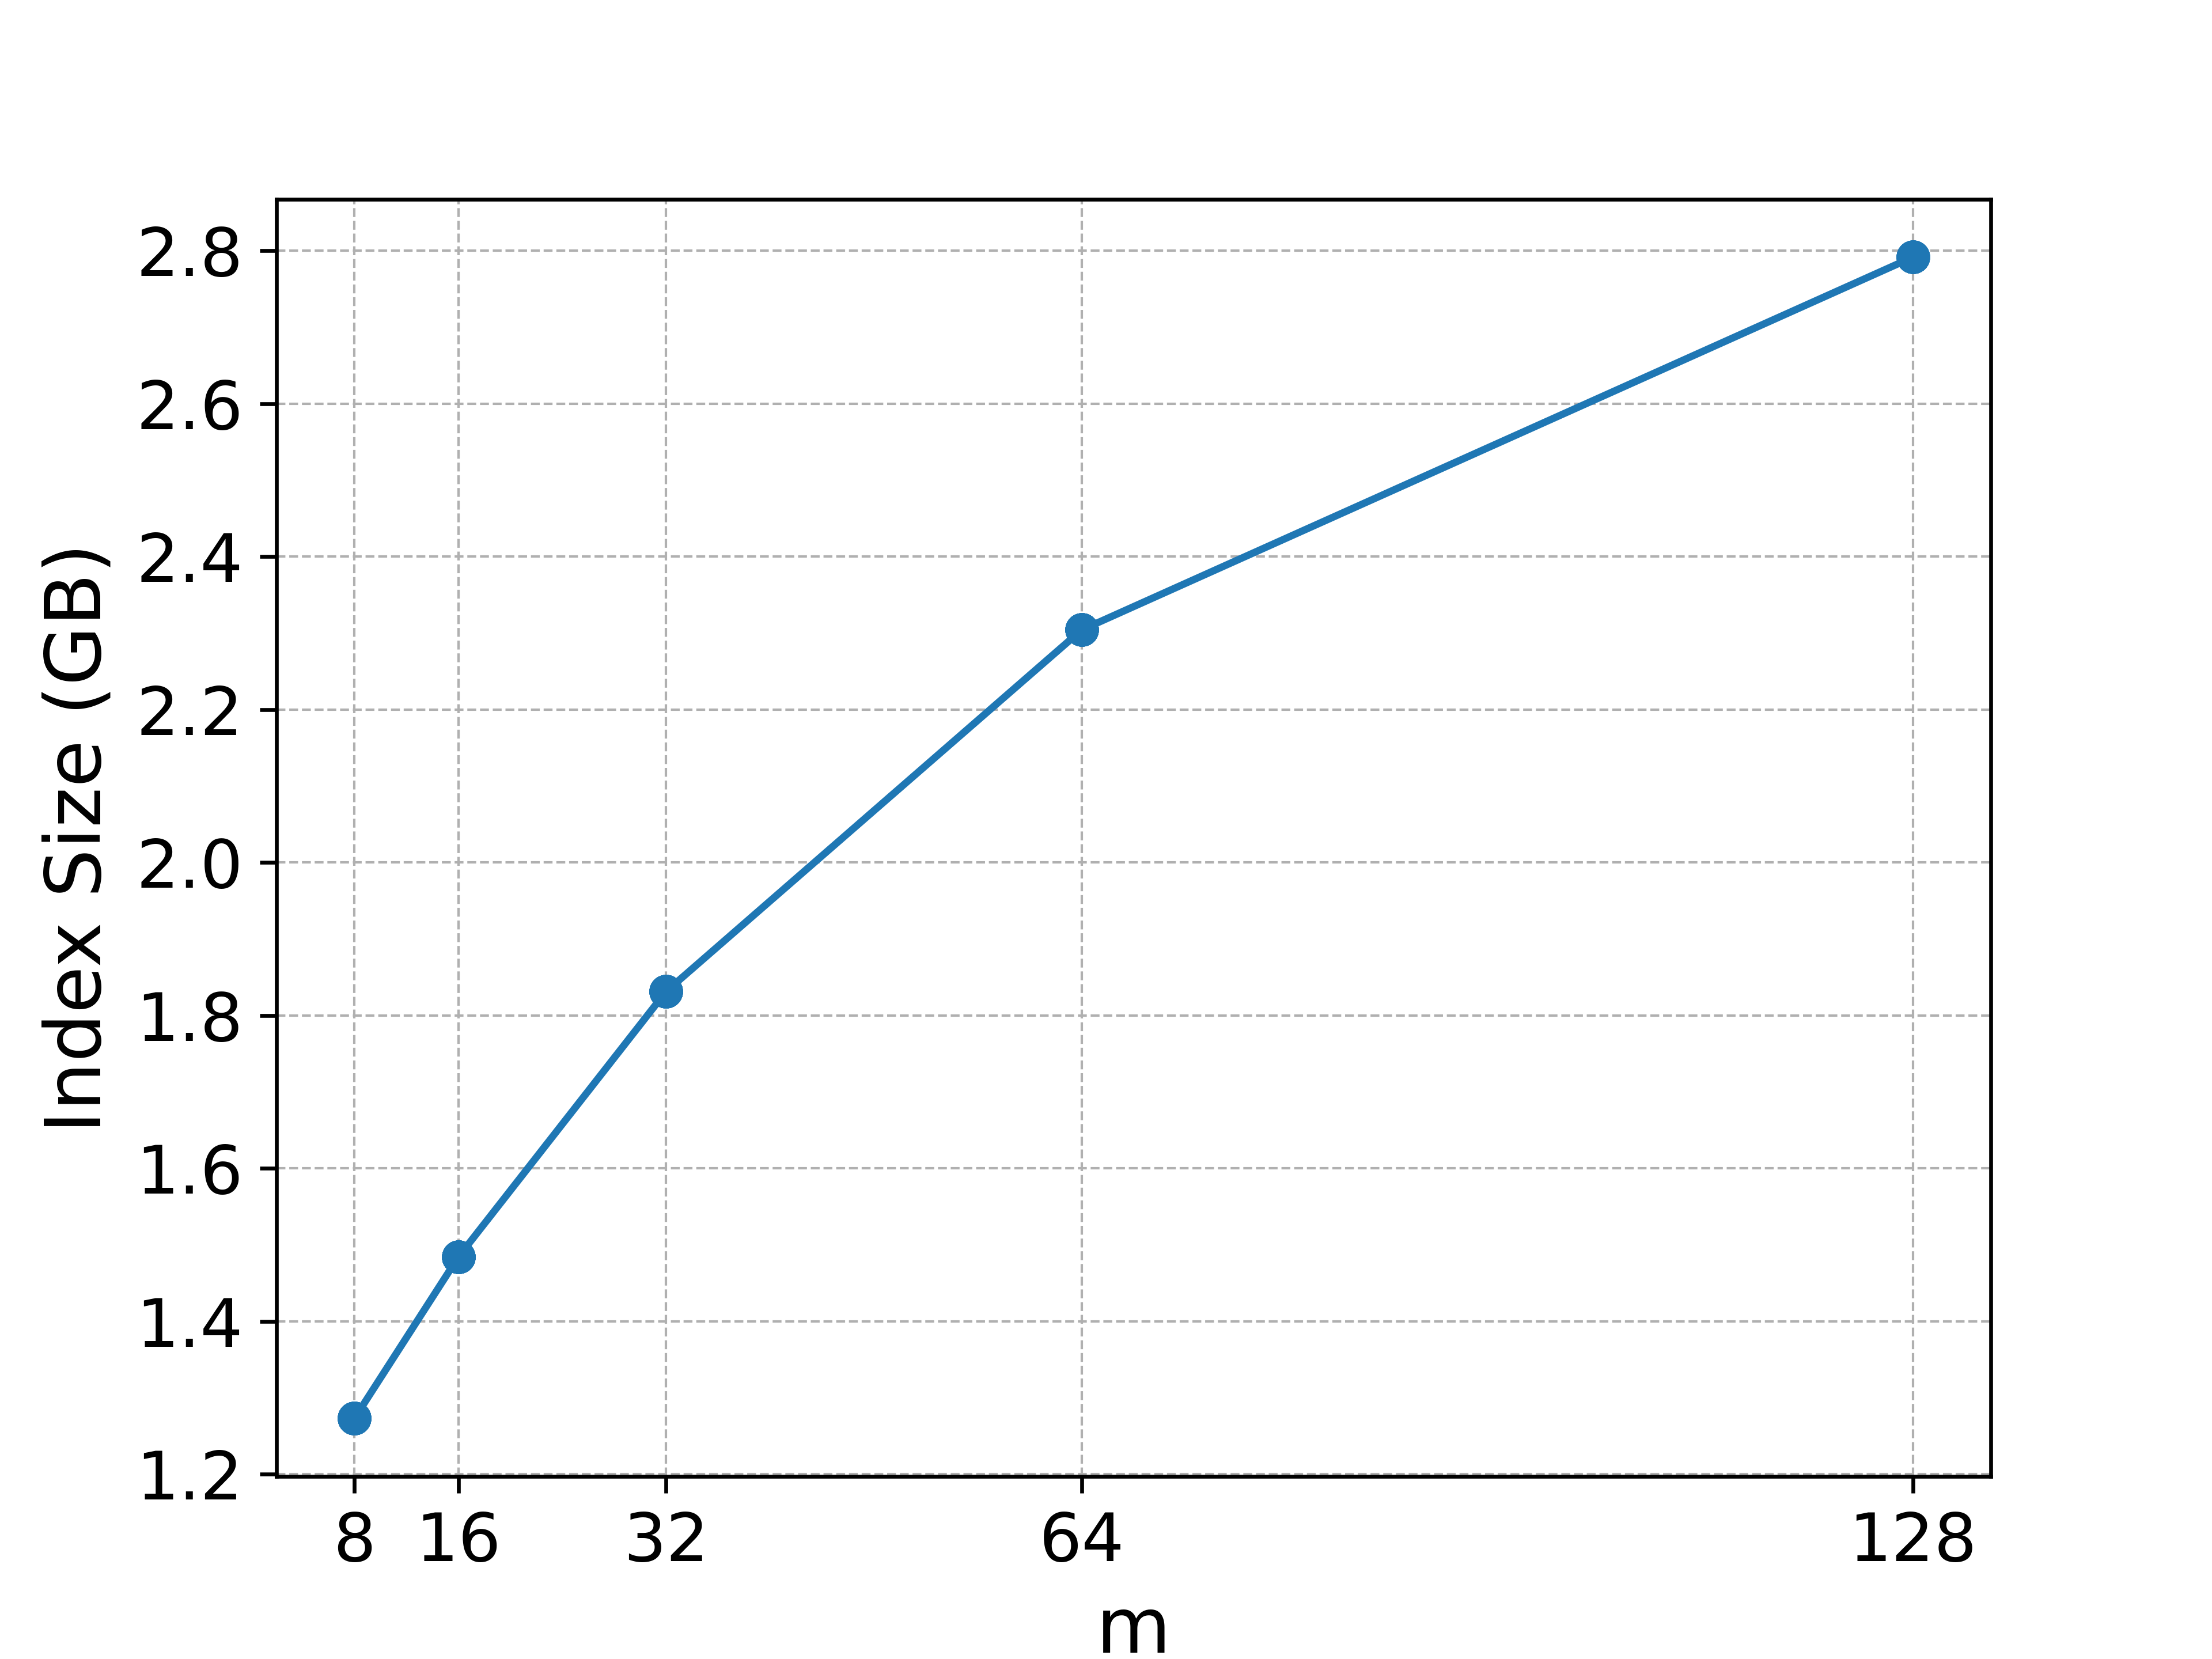
\includegraphics[width=\linewidth]{figs/plots/ablation-m/index_size_vs_m_glove-100.png}
        \caption{Index size vs $m$}
        \label{fig:index-size-ablation-m}
    \end{subfigure}
    
    \medskip

    \begin{subfigure}{0.45\textwidth}
        \centering
        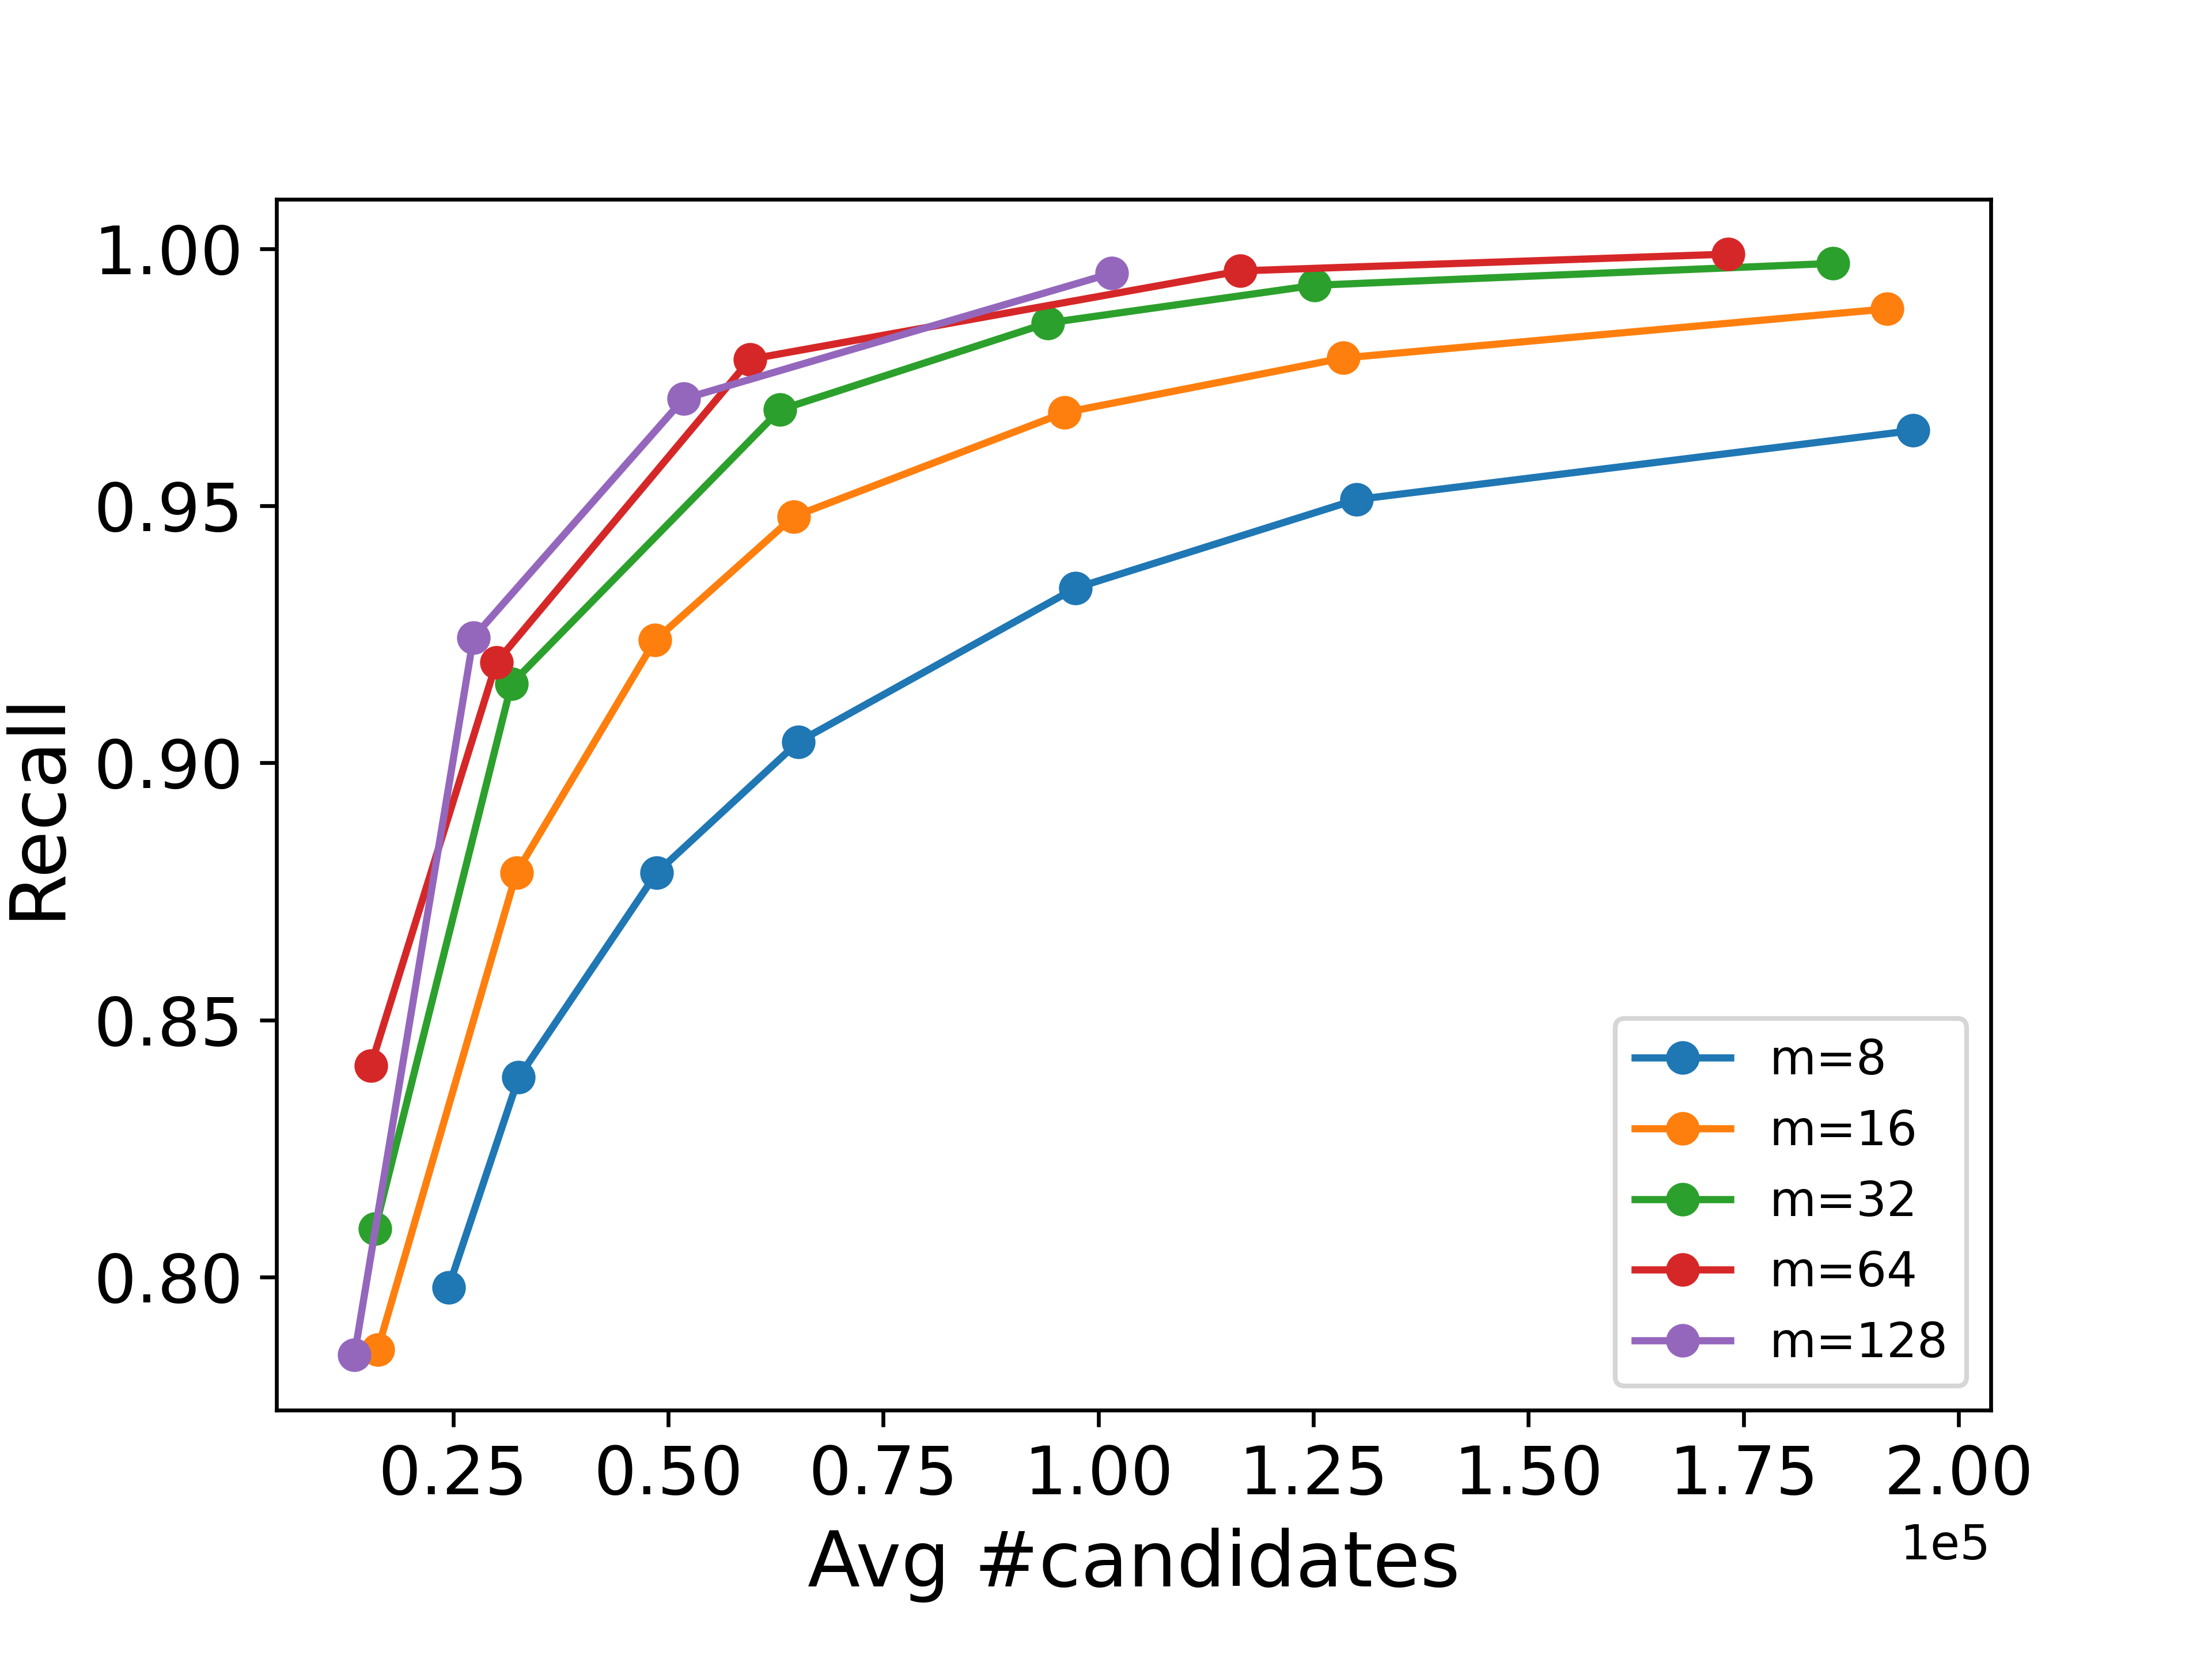
\includegraphics[width=\linewidth]{figs/plots/ablation-m/recall_vs_candidates_glove-100.png}
        \caption{Recall vs average \#candidates per query}
        \label{fig:recall-candidates-ablation-m} 
    \end{subfigure}
    \hfill
    \begin{subfigure}{0.45\textwidth}
        \centering
        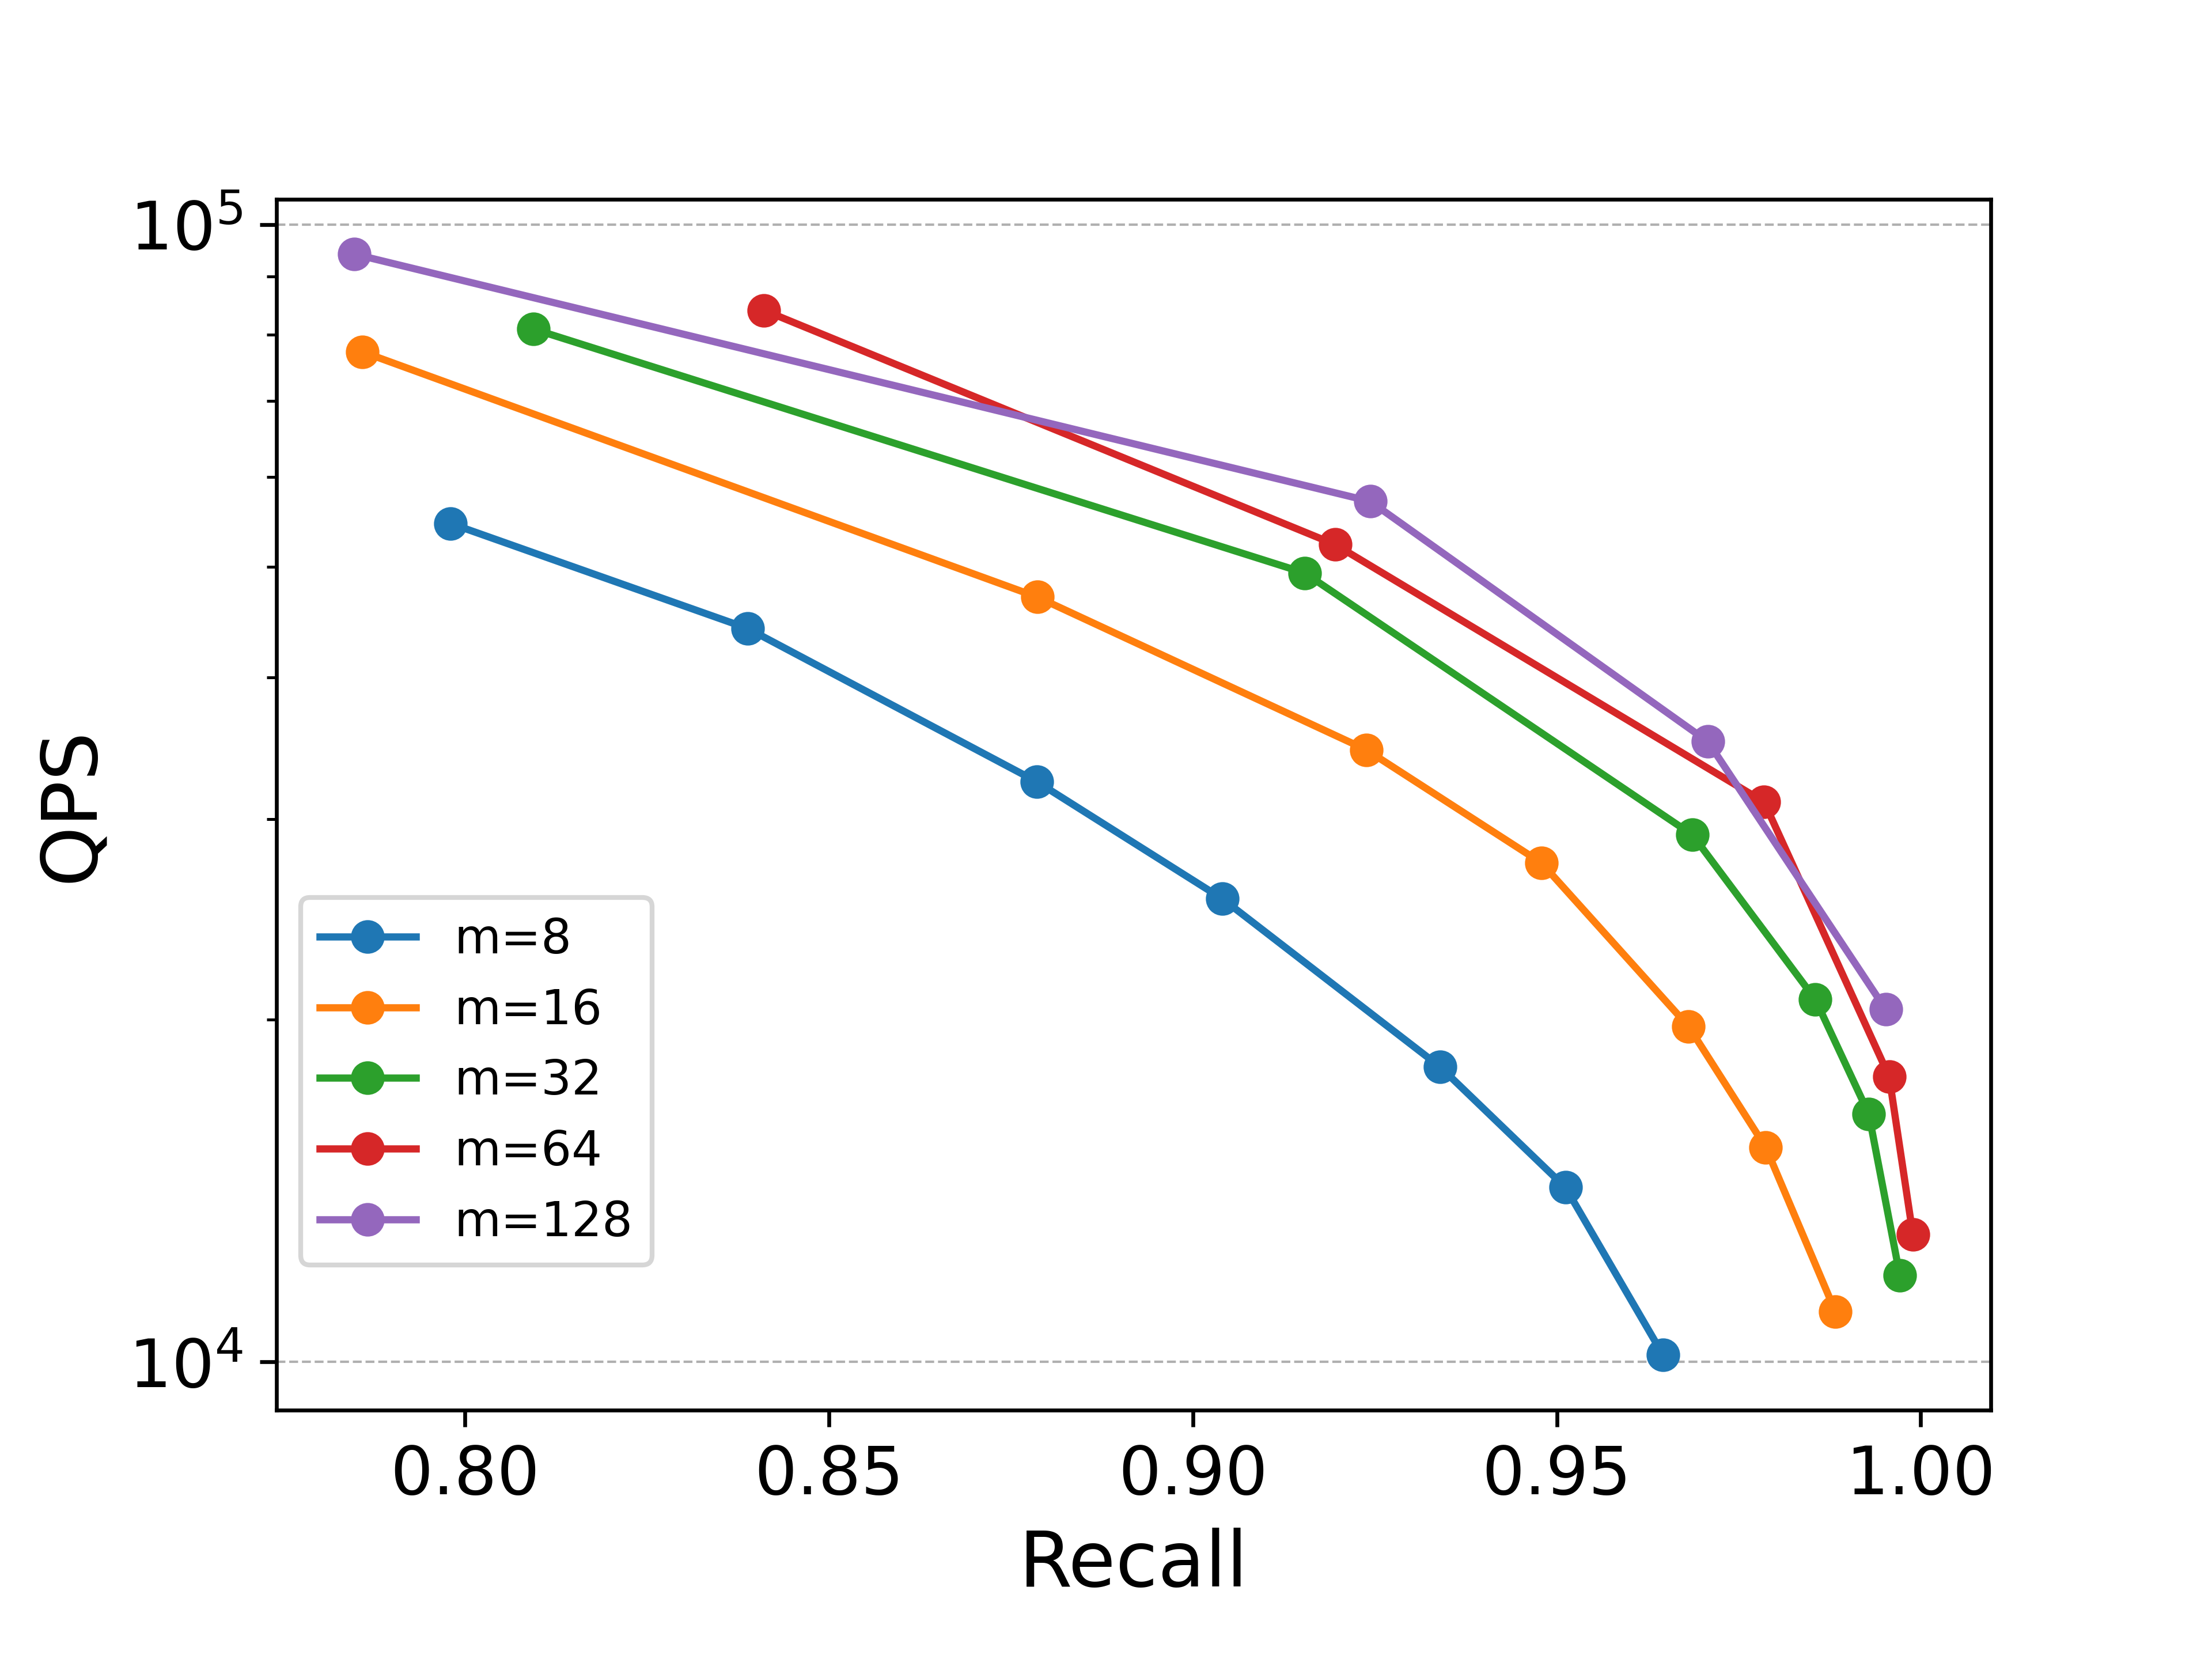
\includegraphics[width=\linewidth]{figs/plots/ablation-m/recall_vs_qps_one_line_per_m_glove-100.png}
        \caption{Recall vs QPS}
        \label{fig:recall-qps-ablation-m} 
    \end{subfigure}

    \caption{Results of ablation study by varying $m$ on \glv.}
    \label{fig:ablation-study-m}
\end{figure}

\subsection{Ablation study of $D$ and $L$ on \glv}
\label{sec:DL-ablation}

We analyse the sensitivity of the index to the parameters $D$ and $L$ on \glv. Throughout the study, we fix $iProbes = 4$ and $m = 8$, $D$ and $L$ according two two complementary sweeps:

\begin{itemize}
    \item Fixed $L$ sweep: Set $L = 256$, and vary $D \in \{128, 192, 256, 392\}$.
    \item Fixed $D$ sweep:
Set $D = 256$, and vary $L \in \{128, 192, 256, 392\}$.
\end{itemize}

For each $(D, L)$ configuration, we vary $qProbes$ over values in the set $V_{qP}$ shown in Eq.~\ref{eq:set-V} (see Sec.~\ref{sec:ablation-glove}). We then restrict attention to the combination of indexing and querying configurations that achieve recall higher than $0.75$. We will briefly discuss indexing performance, before going into more in-depth discussions on querying implications.

\paragraph{Indexing build time and space.}

We report the indexing build times and space of all $(D, L)$ combinations in Tab.~\ref{tab:index-compare-DL}. The index space and build times seem approximately directly proportional to $D$ and $L$. I.e. increasing $D$ or $L$ by a factor increases build time/space by approximately this factor. A notable result is there is symmetry between the build times and space when swapping values of $D$ and $L$, for example, $(D=256, L=192)$ has roughly the same indexing performance as $(D = 192, L = 256)$. 
\begin{table}[]
    \centering

    \begin{subtable}{0.48\textwidth}
        \centering
        \begin{tabular}{c cc}
            $D$ & Build time (s) & Space (GB) \\
            \hline
            128 & 15.8 & 0.63 \\
            192 & 21.4 & 1.26 \\
            256 & 27.7 & 1.96 \\
            392 & 45.5 & 3.47 \\
        \end{tabular}
        \caption{$L = 256$}
    \end{subtable}
    \hfill
    \begin{subtable}{0.48\textwidth}
        \centering
        \begin{tabular}{c cc}
            $L$ & Build time (s) & Space (GB) \\
            \hline
            128 & 15.8 & 0.98 \\
            192 & 22.4 & 1.47 \\
            256 & 27.7 & 1.96 \\
            392 & 45.4 & 3.00 \\
        \end{tabular}
        \caption{$D = 256$}
    \end{subtable}
    
    \caption{Indexing build time and space on \glv comparing fixed $L$ or $D$. }
    \label{tab:index-compare-DL}
\end{table}

\paragraph{Recall and querying speed.} For a fixed $D$, we find no significant benefit in varying $L$. As shown by Fig.\ref{fig:qps-recall-D-ablation-DL}, a larger $L$ generally leads to comparable or lower QPS for the same fixed recall. For recall values greater than $\approx 0.75$, there is little difference between choosing different $L$ values. However, for a fixed $L$, there is are clear trade offs between large and small $D$ values as shown in Fig.~\ref{fig:qps-recall-L-ablation-DL}. For a small $D$, \cf generally has faster QPS for recall less than 0.85, but for very-high recalls around $0.95$, it is more appropriate to use a larger $D$. The order of the \emph{max} recall value that each $D$ curve has corresponds to the ordering of $D$ - which indicates that for a fixed $L$, increasing $D$ can increase the maximum recall attained. 

\alert{I think we need to discuss on like trade-offs more. Like in introduction, we say \cf is good for the GPU - but a 5GB index isn't really all that good for a GPU - there for, we could make some comment on diminishing returns for larger $D$/$L$ - maybe say that you can get good results for a small $D, L$ - maybe compare to FAISS for a small $D, L$ combination - would be good to prove this outright without hand wavy comments "it still gets good performance' }

\paragraph{Quality of candidates.} We found that increasing $D$ or $L$ can generally increase the quality of candidates found from the top buckets to a query. This is non-surprising, a larger $D$ or $L$ increases the diversity and selection of buckets to choose from, and thus makes it more likely the top scoring buckets contain close candidates to a query. This effect is shown in Figures \ref{fig:recall-candidates-fixed-D} and \ref{fig:recall-candidates-fixed-L} - generally a higher $L$ or $D$ allows a higher recall for the same number of candidates. An interesting effect however, is that $D$ seems to matter more than $L$ when increasing candidate quality - there is a larger range in the curves from \ref{fig:recall-candidates-fixed-L} than \ref{fig:recall-candidates-fixed-D}. 

\paragraph{Projections costs.} Our study also revealed that using a larger $D$ or $L$ increases the relative cost of projections (hashing) w.r.t. the total time of querying. To show this, we found the mean percentage of querying time spent doing projections across all indexing query configurations. For a fixed $L$, increasing $D$ from $128$ to $392$ increased this average percentage from $21\%$ to $59\%$ - a $38\%$ change. We found a similar effect for a fixed $D$ and varied $L$.

\alert{For last paragraph. Say that we observe a similar effect of projection costs for a varied $L$ given a fixed $D$. I think needs to link to other paragraphs otherwise it's at risk of being a side-point. Do this last, not that important.}

\alert{Last paragraph at the very least needs to also draw comparison with projection speed ups with a fixed $D$ also!}

\alert{This last paragraph could also help explain the other points. Larger $D$ or $L$ means more hashing cost. This hashing cost pays off for high recall since you much less candidates than other regimes for same recall (which are dominating factor for query speed). This effect is non-linear though, so may be hard to explain easily.}

\begin{figure}[t]
    \begin{subfigure}{0.45\textwidth}
        \centering
        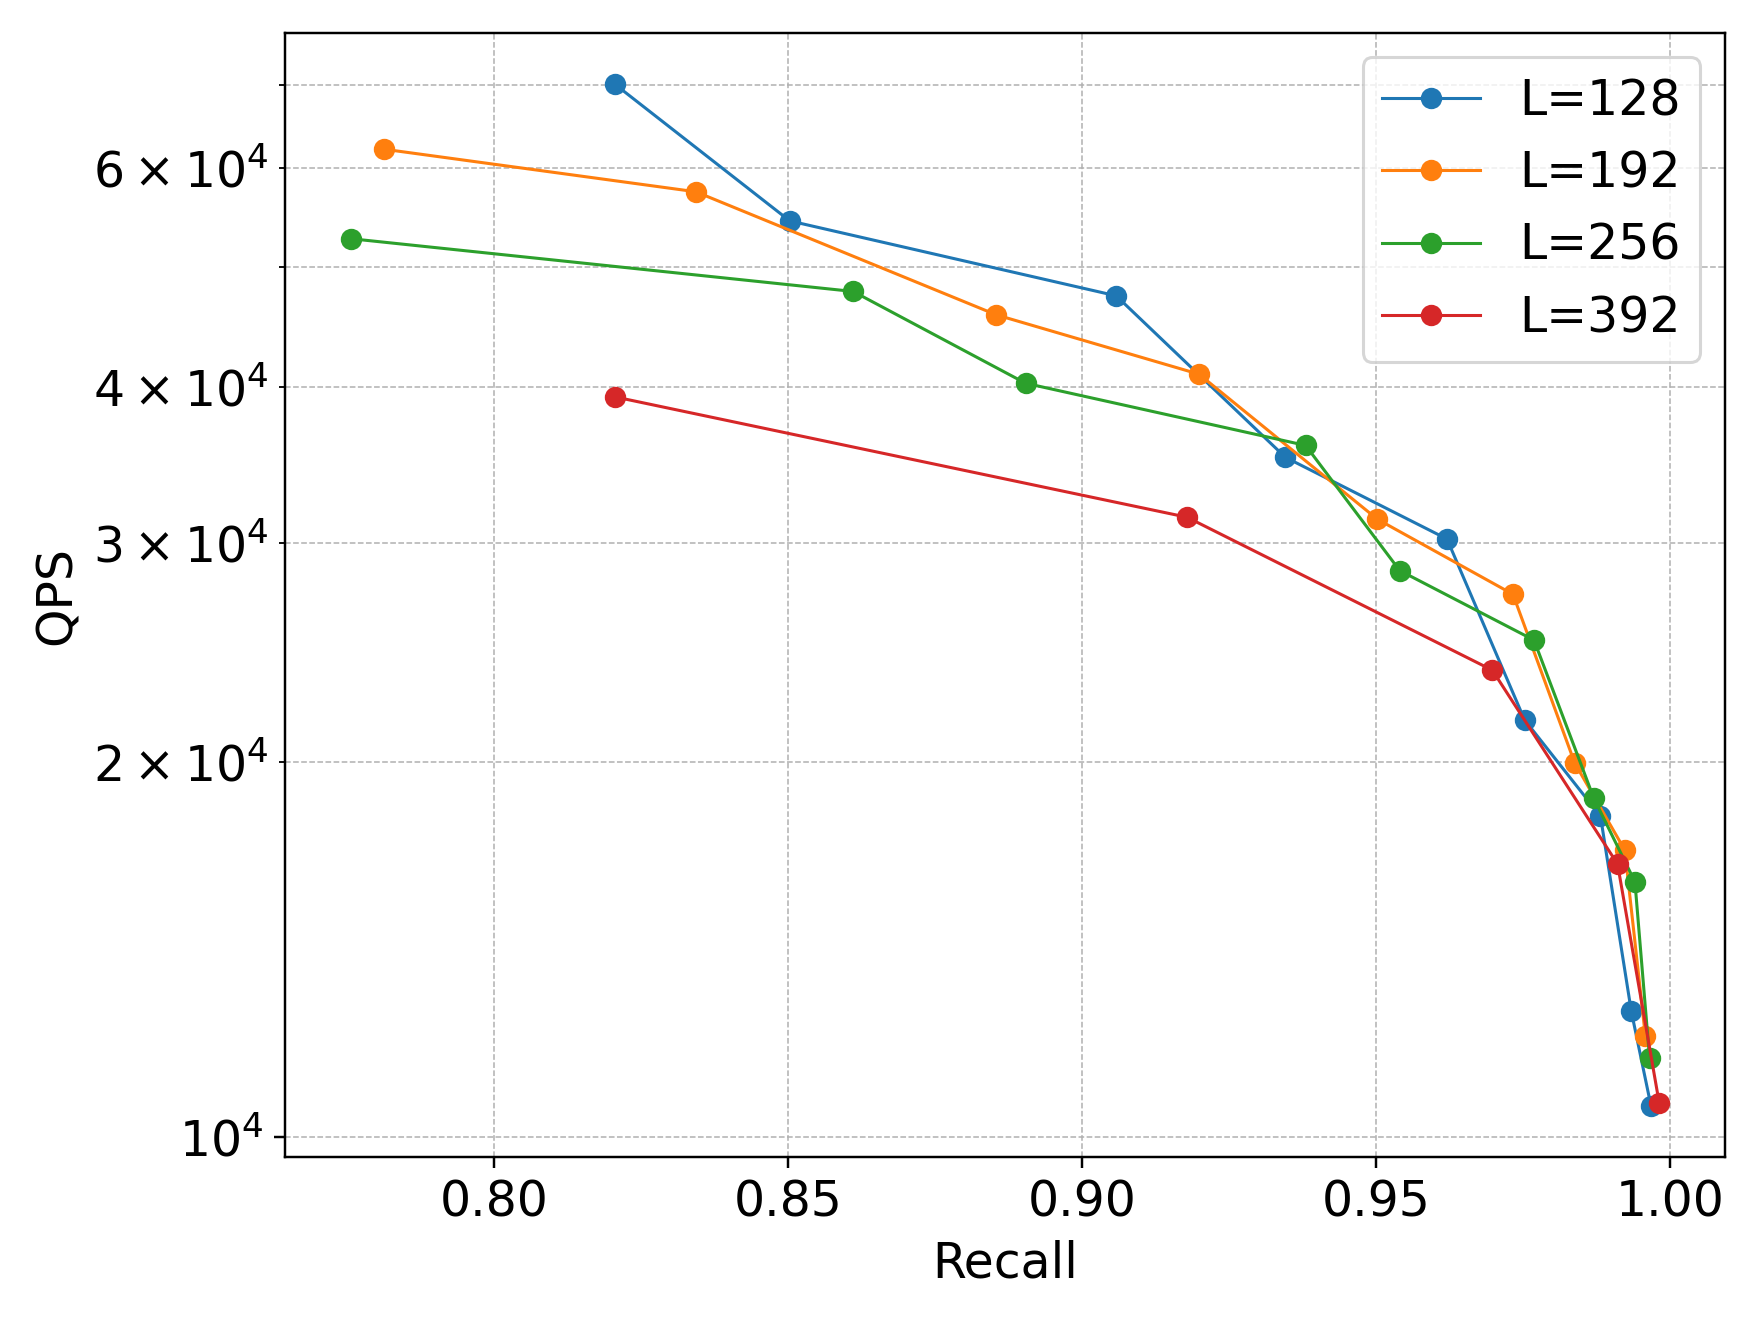
\includegraphics[width=\linewidth]{figs/plots/ablation-DL/glove-100_prenorm_True_qps_vs_recall_fixed_D_256.png}
        \caption{Recall-QPS for $D = 256$, and varying $L$}
        \label{fig:qps-recall-D-ablation-DL}
    \end{subfigure}
    \hfill
    \begin{subfigure}{0.45\textwidth}
        \centering
        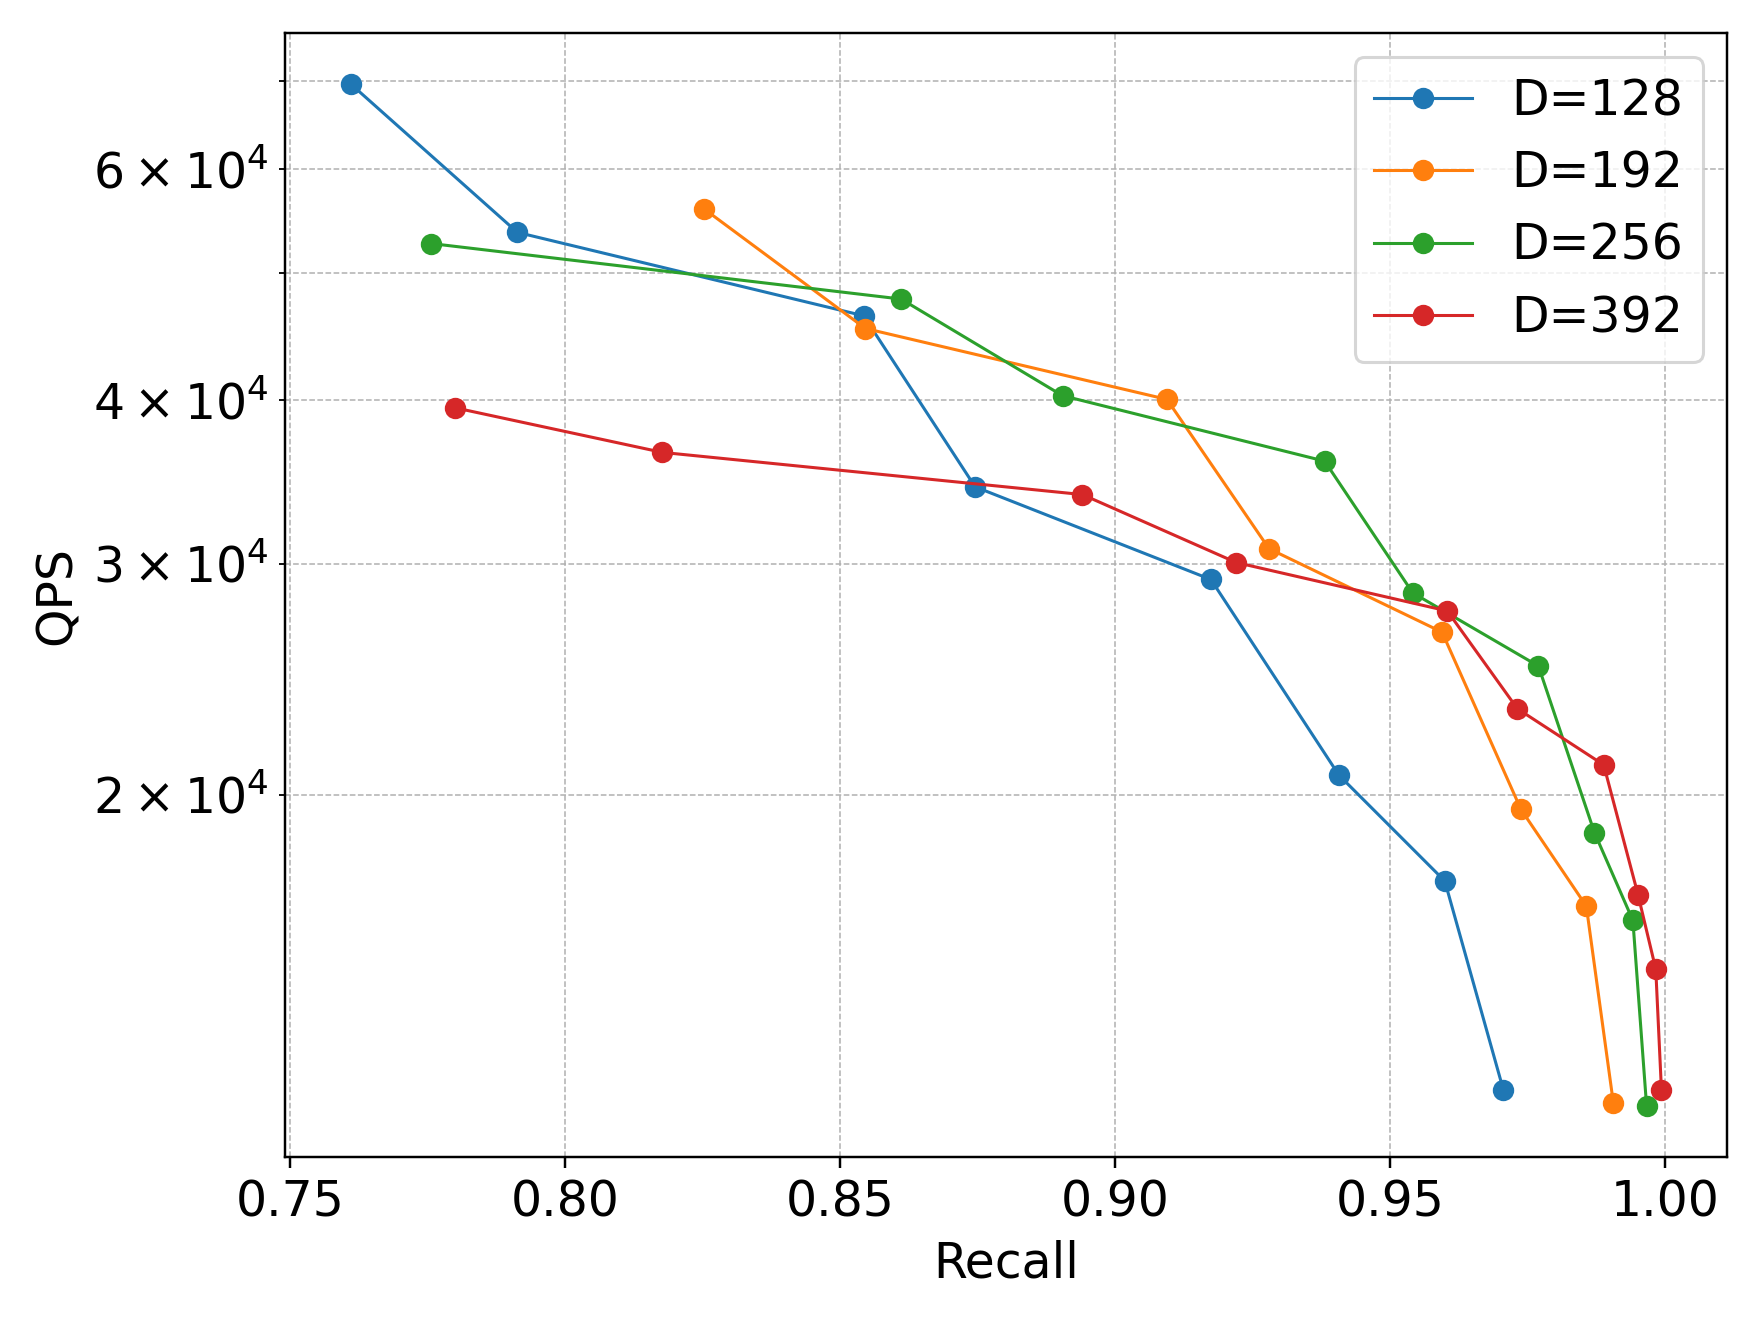
\includegraphics[width=\linewidth]{figs/plots/ablation-DL/glove-100_prenorm_True_qps_vs_recall_fixed_n_repeats_256.png}
        \caption{Recall-QPS for $L = 256$, and varying $D$}
        \label{fig:qps-recall-L-ablation-DL}
    \end{subfigure}

    \caption{Results of QPS vs recall by varying $D$ and $L$ on \glv.}
    \label{fig:ablation-study-DL}
\end{figure}

\begin{figure}[t]
    \begin{subfigure}{0.45\textwidth}
        \centering
        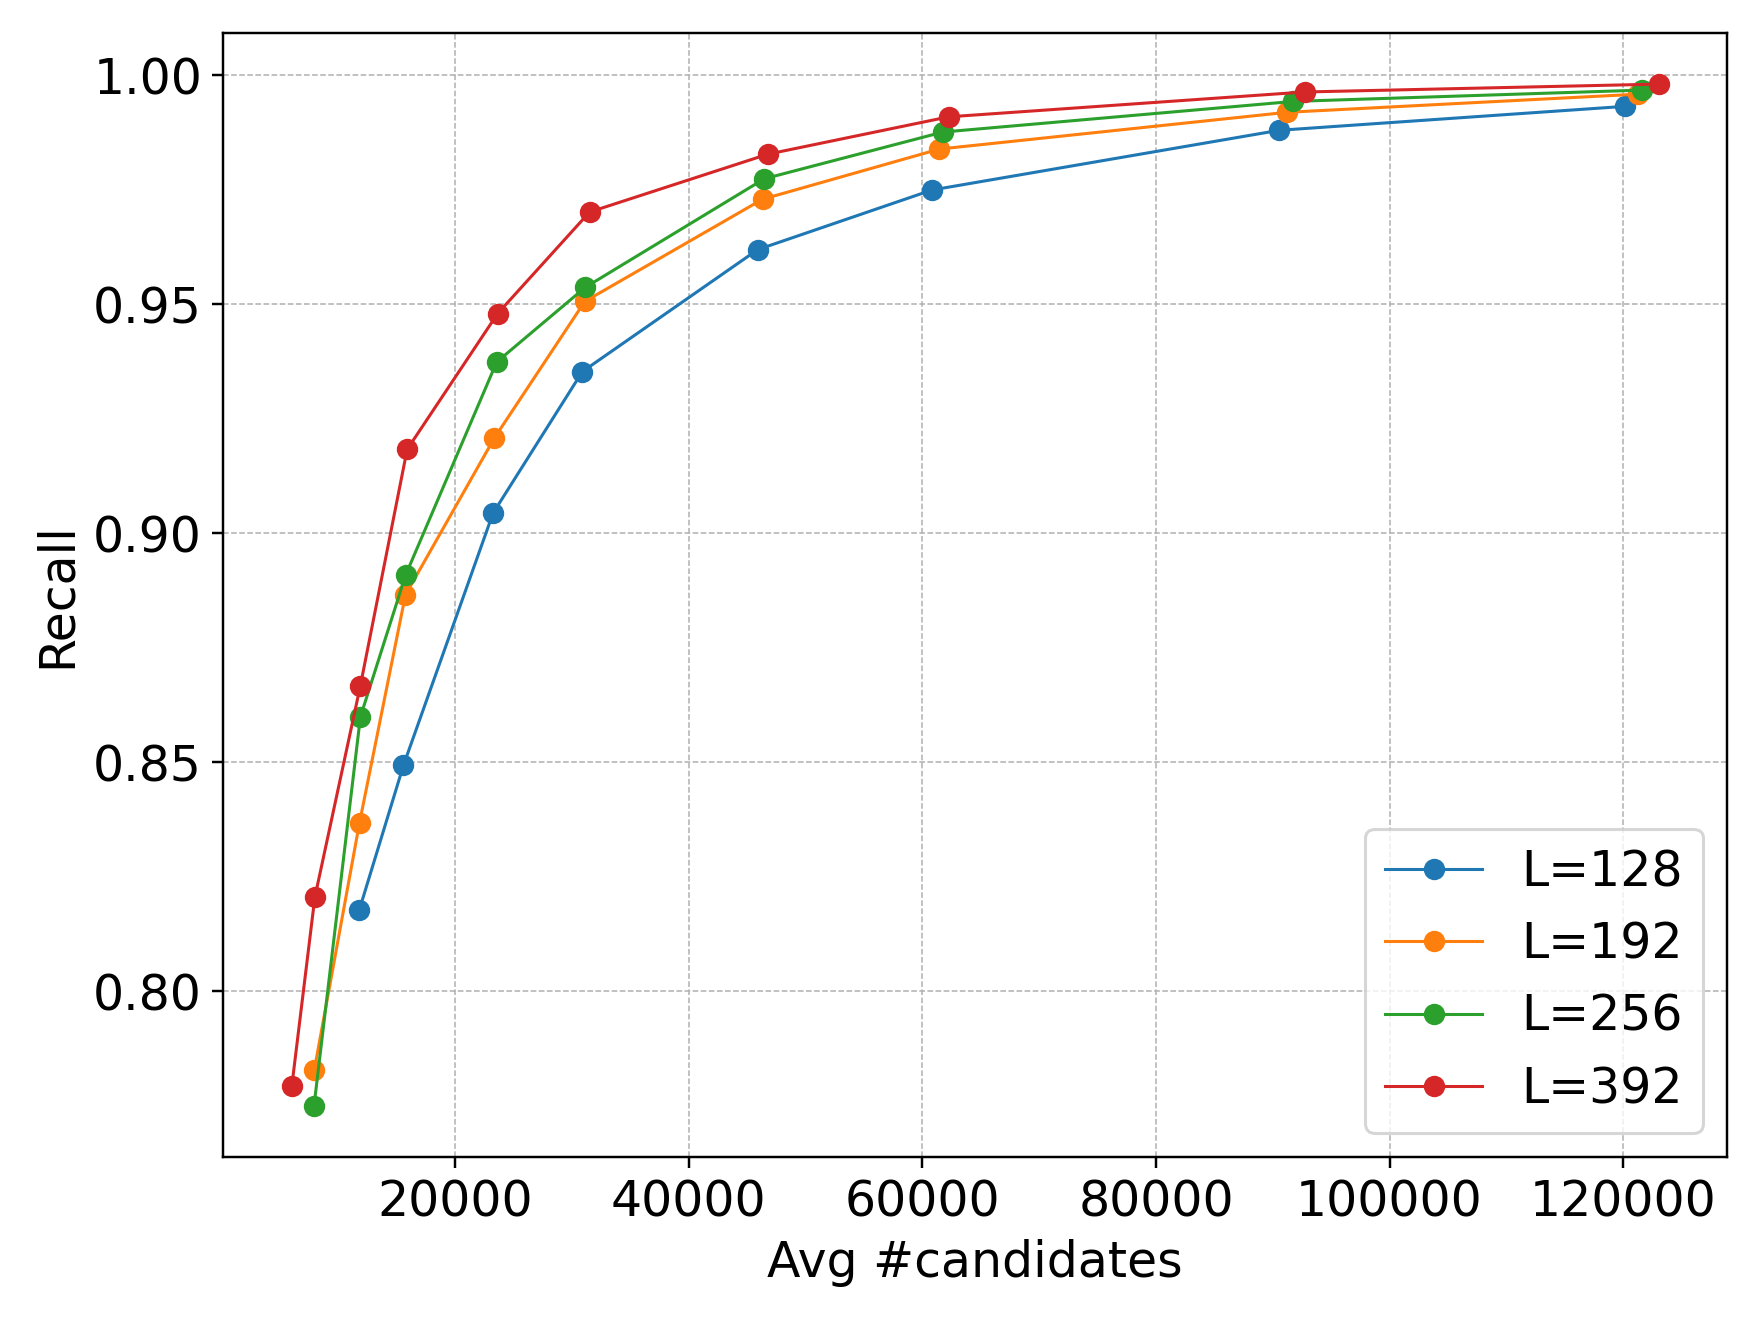
\includegraphics[width=\linewidth]{figs/plots/ablation-DL/glove-100_prenorm_True_recall_vs_avg_candidates_fixed_D_256.png}
        \caption{Recall vs average \#candidates per query. $D=256$ and varied $L$}
        \label{fig:recall-candidates-fixed-D}
    \end{subfigure}
    \hfill
    \begin{subfigure}{0.45\textwidth}
        \centering
        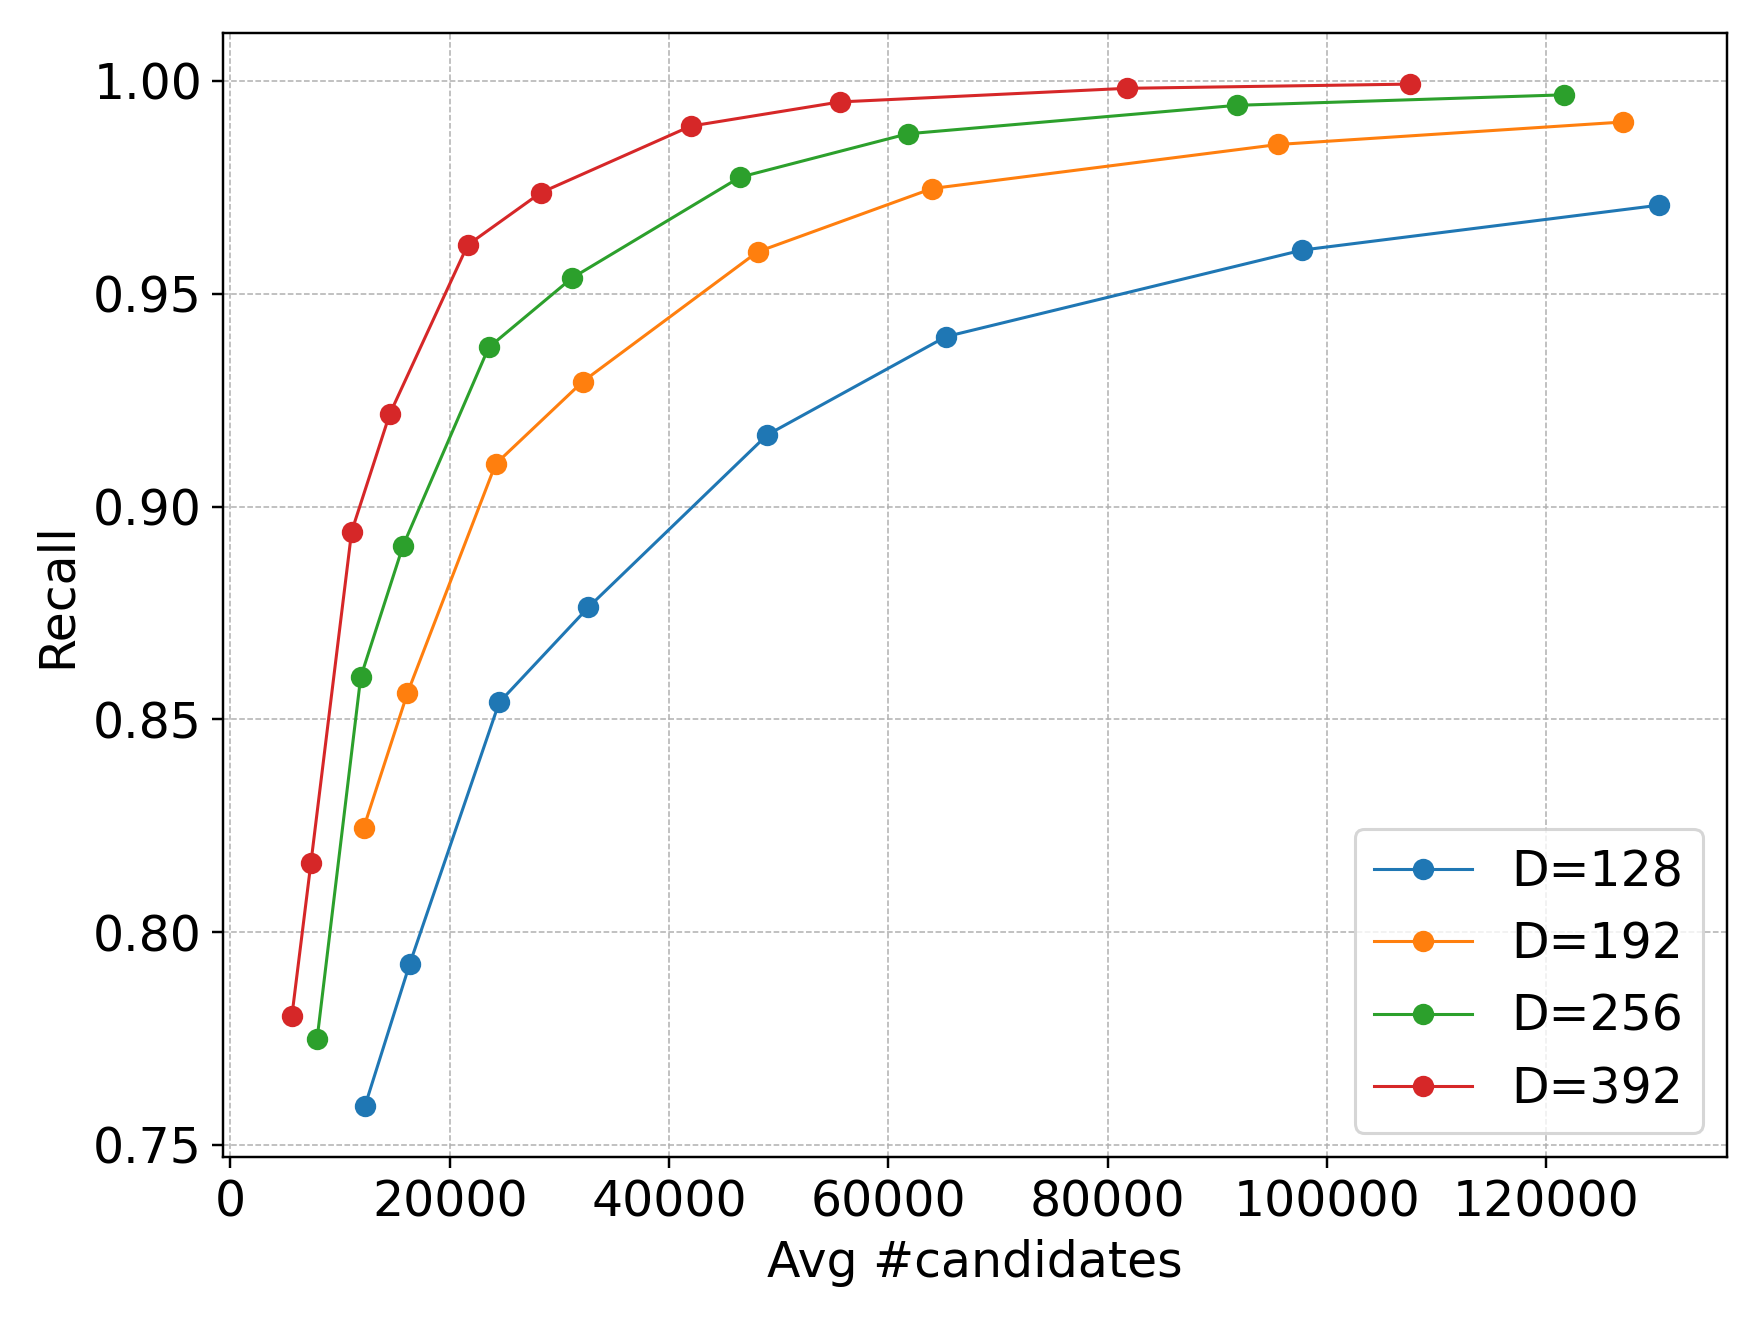
\includegraphics[width=\linewidth]{figs/plots/ablation-DL/glove-100_prenorm_True_recall_vs_avg_candidates_fixed_n_repeats_256.png}
        \caption{Recall vs average \#candidates per query. $L=256$ and varied $D$}
        \label{fig:recall-candidates-fixed-L}
    \end{subfigure}
    
    \medskip
    
    \caption{Results of candidate quality by varying $D$ and $L$ on \glv.}
    \label{fig:ablation-study-DL-candidates}
\end{figure}

% \begin{figure}
%     % \begin{subfigure}{0.45\textwidth}
%     %     \centering
%     %     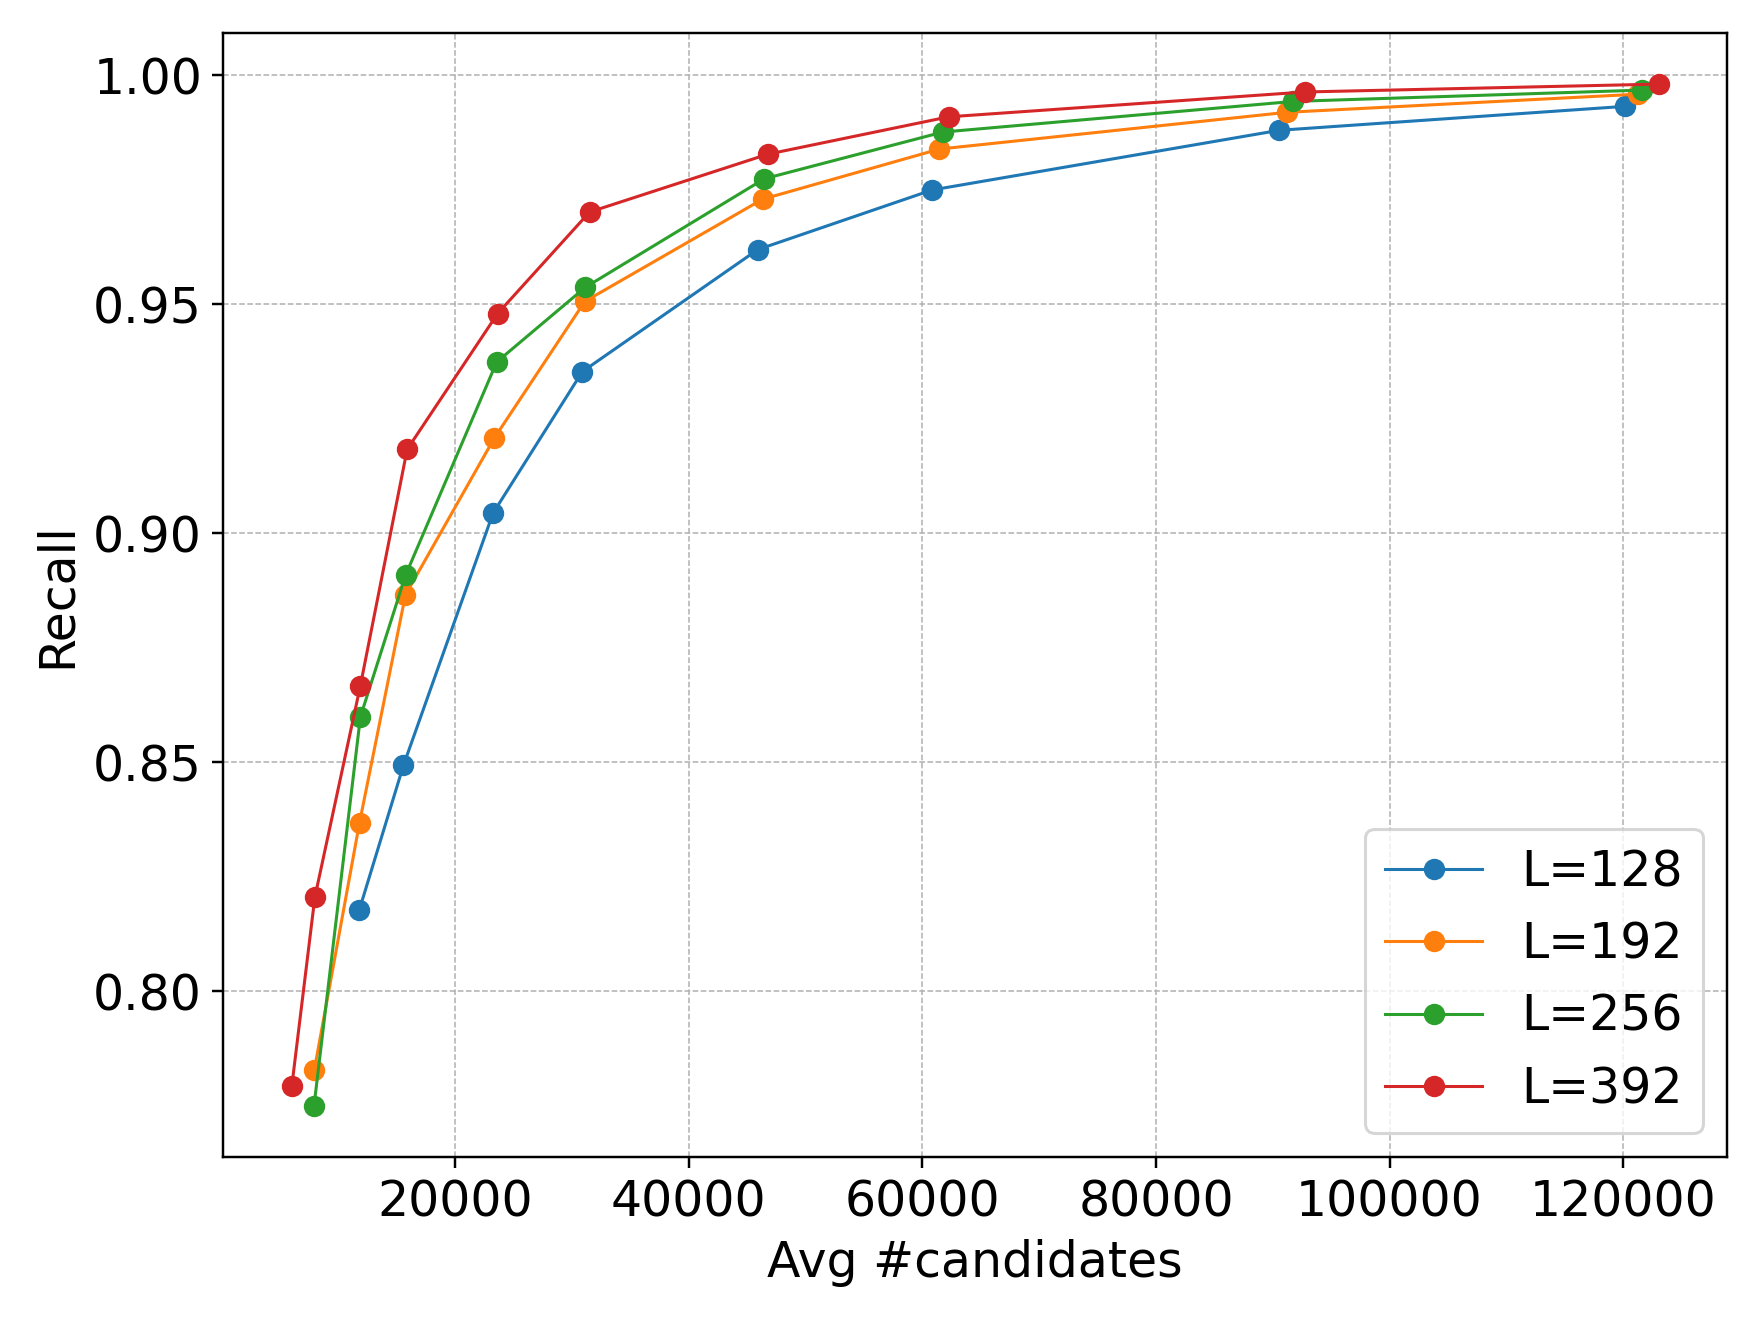
\includegraphics[width=\linewidth]{figs/plots/ablation-DL/glove-100_prenorm_True_recall_vs_avg_candidates_fixed_D_256.png}
%     %     \caption{Recall vs average \#candidates per query. $D=256$ and varied $L$}
%     %     \label{fig:recall-candidates-fixed-D}
%     % \end{subfigure}

%     % \begin{subfigure}{0.45\textwidth}
%     %     \centering
%     %     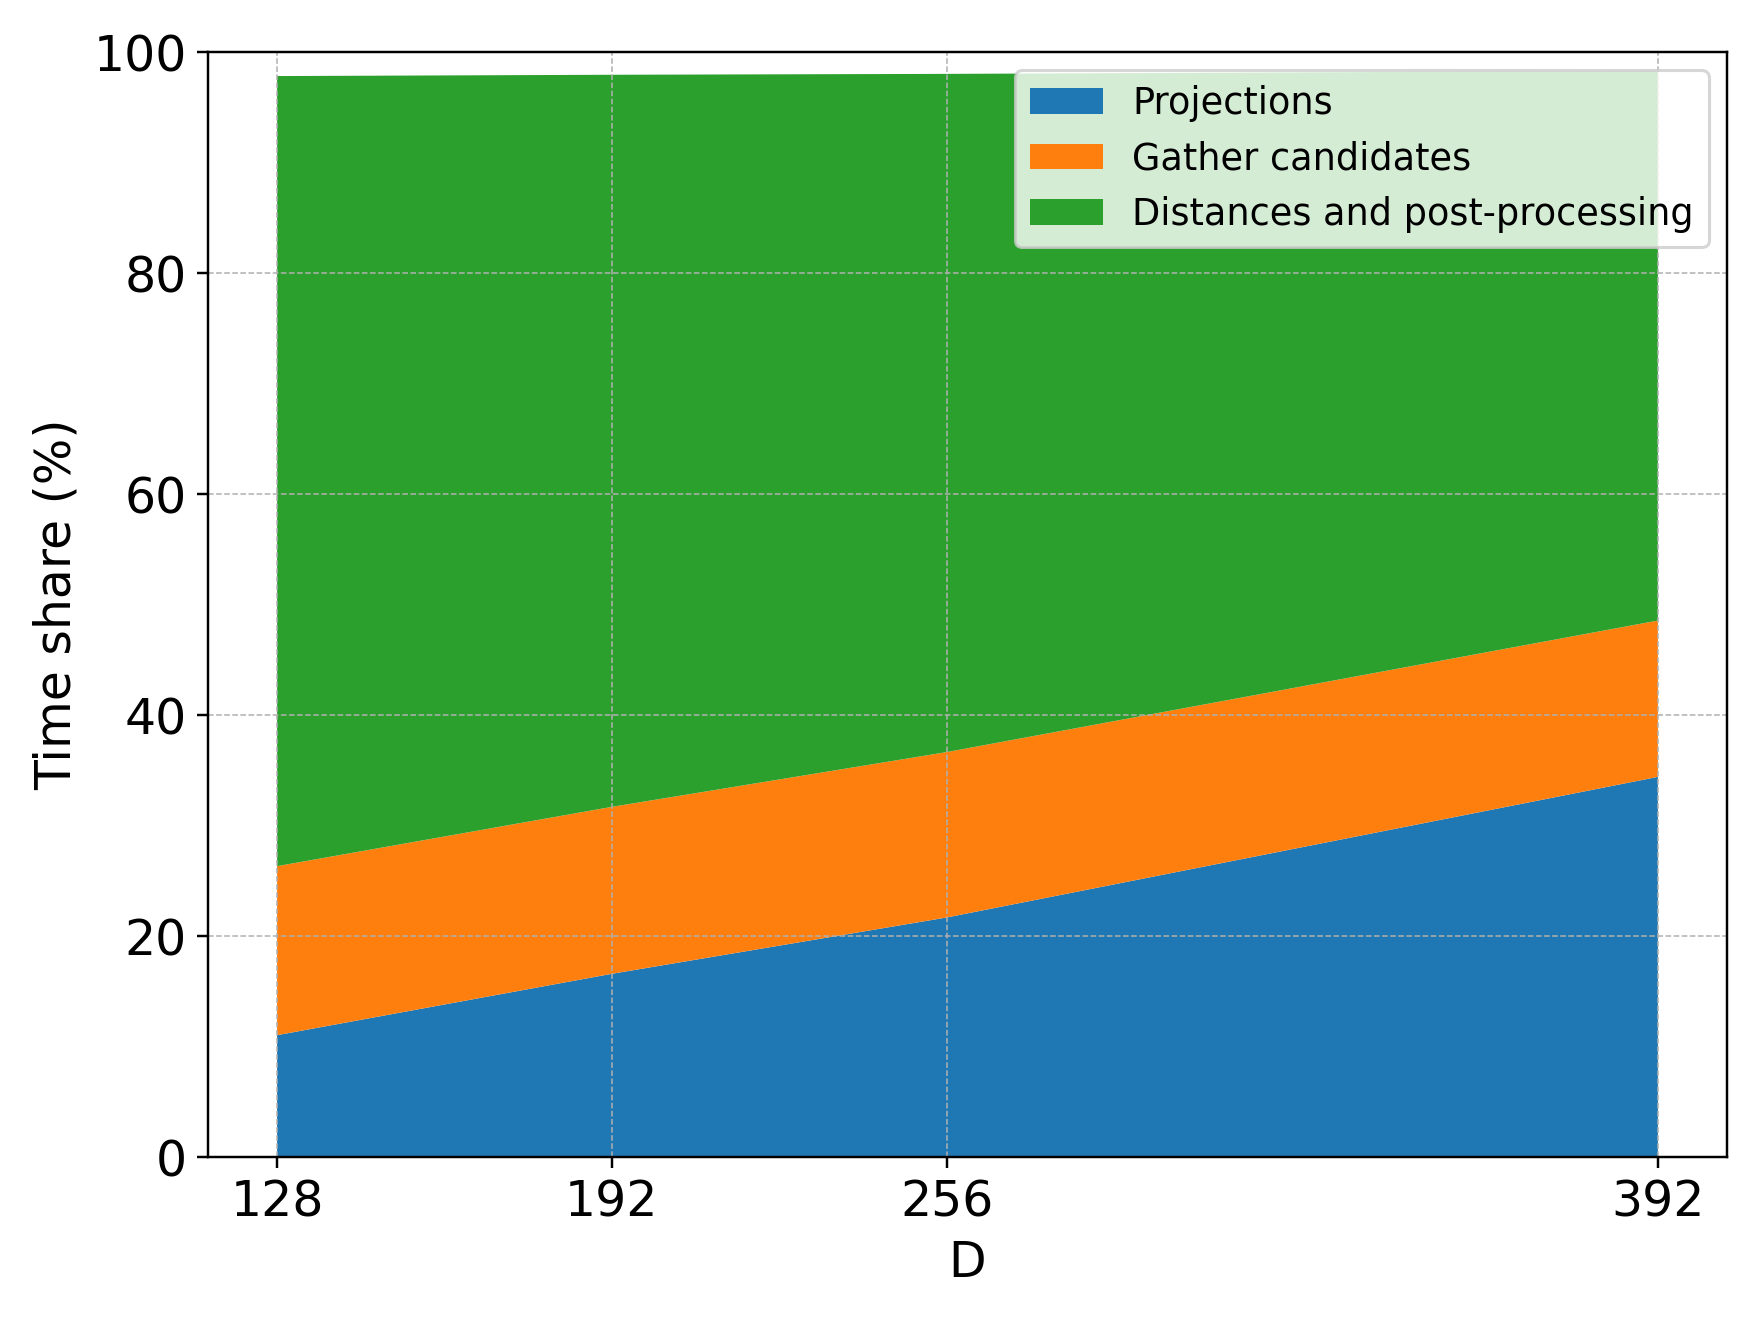
\includegraphics[width=0.5\linewidth]{figs/plots/ablation-DL/query_time_breakdown_fixed_n_repeats_256.png}
%     %     \caption{Breakdown of query runtime components for $qProbes = 12288, D=256$,and varied $L$}
%     %     \label{fig:ablation-study-DL-query-breakdown}
%     % \end{subfigure}
    
%     \centering
%     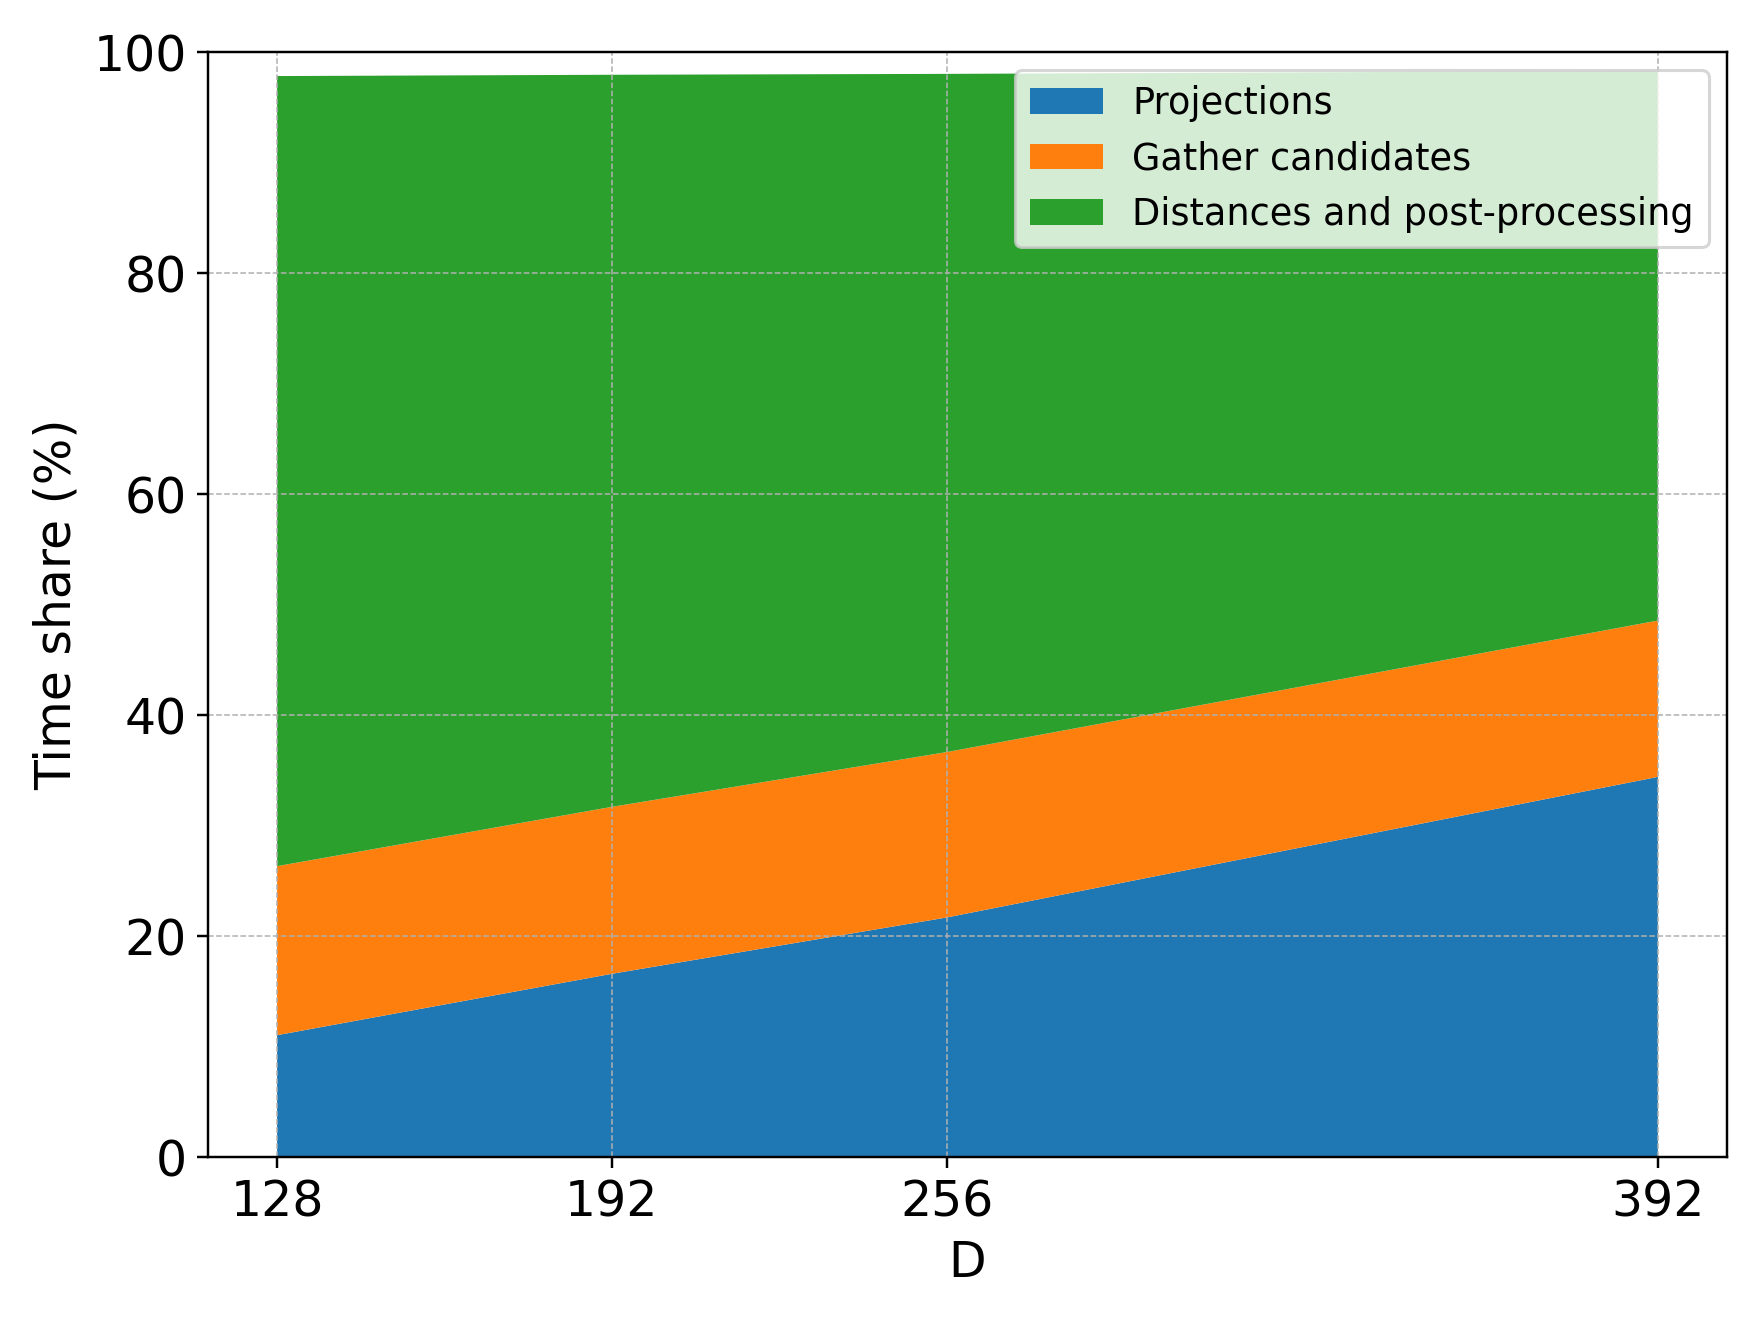
\includegraphics[width=0.5\linewidth]{figs/plots/ablation-DL/query_time_breakdown_fixed_n_repeats_256.png}
%     \caption{Breakdown of query runtime components for $qProbes = 12288, D=256$,and varied $L$}
%     \label{fig:ablation-study-DL-query-breakdown}
    
% \end{figure}

% \subsection{Profiling analysis on GloVe-100}

% \alert{This section is pre-liminary - not sure if we are going to totally look into it}

% \alert{Can use this section to go into a componenent analysis - show what are the dominating components interms of runtime}

% \alert{Can use profiling results to help paint a better picture}

\section{Conclusions}

\alert{Summarise the implementation and the contributions of this paper}

\alert{Summarise future directions}

\bibliographystyle{plain}
\bibliography{refs}

\end{document}
